\documentclass{rapportENSAM}

\setlength{\emergencystretch}{3em}

\usepackage{rotating}

% Package spécifique local
\usepackage{rapid-listings}

\begin{document}


% Informations du document

\ecole{École Nationale Supérieure d'Arts et Métiers}
\titre{TrajCenter v2.0 -- Manuel utilisateur}
\contexte{Manuel utilisateur et guide d'intégration}
\sujet{TrajCenter avec ABB Robot Web Services}

\labelAuteur{Auteurs :}
\auteur{
    Josselin \textsc{Schumacker}\\
    Clément \textsc{Racinet}
}

% Superviseur vide : aucun bloc inutile à droite
\superviseur{}



% Page de garde et Sommaire



\fairepagedegarde

\fairemargesintro



% Avant-propos



\renewcommand{\abstractname}{Avant-propos}
\begin{abstract}
Ce document présente l'utilisation de TrajCenter v2.0 pour la conversion,
la gestion et le transfert de trajectoires industrielles vers un robot ABB
RobotWare 6.x.

Il s'adresse principalement aux utilisateurs souhaitant :
\begin{itemize}
    \item convertir des trajectoires au format TrajCenter ;
    \item utiliser l'interface terminal ou la ligne de commande ;
    \item lancer la supervision Python via ABB Robot Web Services ;
    \item exploiter les trajectoires chargées depuis un programme RAPID.
\end{itemize}

TrajCenter v2.0 repose exclusivement sur ABB Robot Web Services. L'ancien
protocole TCP de TrajCenter v1 n'est plus utilisé.
\end{abstract}

\newpage



% Sommaires



\tableofcontents
\newpage

% % Commenter les listes inutiles au besoin
% \listoffigures
% \newpage

% \listoftables
% \newpage

% \lstlistoflistings
% \newpage

\fairemarges




% Corps du document



%------------------------------------------------------------------------------
% Partie I : Introduction et démarrage rapide
%------------------------------------------------------------------------------

\section*{Introduction}
\addcontentsline{toc}{section}{Introduction}
\label{sec:introduction}

TrajCenter v2.0 est un outil de préparation, de stockage et de transfert de trajectoires industrielles vers un robot ABB fonctionnant sous RobotWare~6.x (testé uniquement sur 6.08 et 6.15). Il permet de convertir plusieurs formats de fichiers en une archive commune portant l'extension \texttt{.trajcenter}, puis de transférer la trajectoire sélectionnée vers le contrôleur au moyen d'ABB Robot Web Services.

TrajCenter peut être utilisé selon deux modes complémentaires :

\begin{itemize}
    \item \textbf{hors ligne}, sur un poste de préparation, pour convertir,
    consulter et exporter des trajectoires sans connexion à un robot ;
    \item \textbf{en ligne}, sur un PC connecté à la cellule, pour superviser
    les échanges avec le contrôleur ABB et charger une trajectoire dans le
    module RAPID \texttt{TRAJCENTER}.
\end{itemize}

La conversion reste indépendante du robot. Une archive \texttt{.trajcenter} peut donc être préparée, vérifiée et conservée sans accès au contrôleur. Lors du transfert, TrajCenter prend en compte les tools, les workobjects, les valeurs par défaut et les types de process exposés par la
cellule. Les limites prises en charge par Python sont également vérifiées avant l'écriture, tandis que les dimensions du module RAPID constituent la limite finale côté contrôleur.

Le fonctionnement général repose sur quatre éléments :

\begin{itemize}
    \item les fichiers sources, par exemple CSV, Excel, APT ou RAPID ;
    \item le store local contenant les archives \texttt{.trajcenter} ;
    \item le superviseur Python, chargé des échanges avec le contrôleur ;
    \item le module système RAPID \texttt{TRAJCENTER.sys}, chargé dans la
    tâche robot configurée.
\end{itemize}

La communication entre le PC et le contrôleur utilise exclusivement ABB Robot Web Services. L'ancien serveur TCP et le protocole de communication de TrajCenter v1 ne sont plus utilisés.

Le présent manuel s'adresse principalement aux utilisateurs, automaticiens et roboticiens chargés de préparer les trajectoires, de configurer la connexion, de démarrer la supervision et d'exploiter les données chargées depuis un programme RAPID. Les opérations de développement interne du logiciel ne sont abordées que lorsqu'elles sont nécessaires à l'intégration ou au diagnostic.

La section suivante présente un premier cycle d'utilisation complet. Les sections ultérieures détaillent l'installation, la configuration, les commandes disponibles, l'utilisation de l'interface terminal et l'intégration dans un programme RAPID.


%------------------------------------------------------------------------------
% Partie II : Démarrage rapide
%------------------------------------------------------------------------------

\section{Démarrage rapide}
\label{sec:quick-start}

Cette section permet de réaliser un premier essai complet de TrajCenter : installation du logiciel, configuration de la connexion, conversion d'un fichier, démarrage du superviseur puis demande de chargement depuis RAPID.

La procédure utilise l'environnement Pixi \texttt{full}, qui contient à la fois les outils locaux, l'interface terminal et le client ABB Robot Web Services.

Dans ce manuel, le terme \og store local \fg{} désigne le répertoire contenant
les archives \texttt{.trajcenter}.

\subsection{Conditions préalables}
\label{subsec:quick-start-prerequisites}

Avant de commencer, vérifier les points suivants :

\begin{itemize}
    \item Pixi est installé sur le PC ;
    \item le dépôt TrajCenter est disponible localement ;
    \item le PC peut joindre le contrôleur ABB sur le réseau ;
    \item ABB Robot Web Services est accessible sur le contrôleur ;
    \item un compte RWS disposant des autorisations nécessaires est disponible ;
    \item le fichier \texttt{TRAJCENTER.sys} est chargé comme module système
    dans la tâche RAPID utilisée, généralement \texttt{T\_ROB1} ;
    \item la configuration RAPID contient les tools et workobjects nécessaires
    à la trajectoire, ou des valeurs par défaut adaptées ;
    \item les premiers essais peuvent être réalisés dans RobotStudio ou dans
    des conditions de sécurité adaptées sur la cellule réelle.
\end{itemize}

Le chargement réussi d'une trajectoire ne garantit ni l'absence de collision, ni l'accessibilité des positions, ni la sécurité de son exécution. La trajectoire doit être vérifiée avant tout mouvement réel.

\subsection{Étape 1 -- Installer TrajCenter}
\label{subsec:quick-start-installation}

Depuis la racine du dépôt, installer l'environnement complet :

\begin{lstlisting}[
    language=bash,
    caption={Installation rapide de TrajCenter},
    label={lst:quick-start-installation}
]
pixi install -e full
\end{lstlisting}

Vérifier ensuite l'installation et la disponibilité du support ABB :

\begin{lstlisting}[
    language=bash,
    caption={Vérification de l'installation},
    label={lst:quick-start-installation-check}
]
pixi run -e full trajcenter version
pixi run -e full trajcenter robot check
\end{lstlisting}

Lorsque le client ABB est disponible, la seconde commande affiche :

\begin{lstlisting}[
    language={},
    caption={Résultat attendu de la vérification ABB},
    label={lst:quick-start-robot-check-result}
]
Robot ABB API available.
\end{lstlisting}

Cette vérification confirme que les dépendances logicielles sont installées. Elle ne teste pas encore la connexion avec le contrôleur.

\subsection{Étape 2 -- Créer le fichier de configuration}
\label{subsec:quick-start-configuration}

Créer à la racine du projet un fichier nommé, par exemple, \texttt{robot.env}. Adapter son contenu à la cellule utilisée :

\begin{lstlisting}[
    language={},
    caption={Configuration minimale du PC de cellule},
    label={lst:quick-start-env-file}
]
# Connexion ABB Robot Web Services
RWS_HOST=192.168.125.1
RWS_PORT=80
RWS_USER="Default User"
RWS_PASSWORD=robotics
RWS_TIMEOUT=10.0

# Localisation du module RAPID TrajCenter
TRAJCENTER\_RWS\_TASK=T_ROB1
TRAJCENTER\_RWS\_MODULE=TRAJCENTER

# Store local utilise par le superviseur
TRAJCENTER_STORE_ROOT=trajectory_store

# Comportement du superviseur
TRAJCENTER_MASTERSHIP_RETRIES=3
TRAJCENTER_LOG_LEVEL=INFO
\end{lstlisting}

Les valeurs doivent être adaptées comme suit :

\begin{itemize}
    \item \texttt{RWS\_HOST} contient l'adresse IP ou le nom d'hôte du
    contrôleur ;
    \item \texttt{RWS\_PORT} contient le port HTTP utilisé par RWS ;
    \item \texttt{RWS\_USER} et \texttt{RWS\_PASSWORD} contiennent les
    identifiants du compte ABB ;
    \item \texttt{TRAJCENTER\_RWS\_TASK} désigne la tâche dans laquelle le
    module système est chargé ;
    \item \texttt{TRAJCENTER\_RWS\_MODULE} contient le nom du module système ;
    \item \texttt{TRAJCENTER\_STORE\_ROOT} désigne le répertoire contenant les
    archives disponibles pour le robot.
\end{itemize}

Le fichier contenant les identifiants ne doit pas être versionné ni transmis avec des mots de passe de production.

Lorsqu'une option est également fournie dans la ligne de commande, elle remplace la valeur correspondante du fichier de configuration. La priorité générale est donc : l'argument de ligne de commande puis la variable d'environnement ou fichier \texttt{.env} puis la valeur par défaut.


Les dimensions des tableaux RAPID et les capacités du protocole ne doivent pas être ajoutées au fichier \texttt{robot.env}. Elles sont définies dans le module RAPID. La version Python utilise de son côté un profil de protocole compatible pour valider les transferts avant l'écriture.

Dans la version actuelle, le superviseur ne compare pas automatiquement toutes les dimensions du module RAPID avec le profil Python au démarrage. Le module RAPID doit donc être déployé dans une version compatible avec la version de TrajCenter utilisée sur le PC.


\subsection{Étape 3 -- Préparer la configuration RAPID}
\label{subsec:quick-start-rapid-configuration}

Le module \texttt{TRAJCENTER.sys} doit être chargé dans la tâche indiquée par \texttt{TRAJCENTER\_RWS\_TASK}. Le nom du module doit correspondre à \texttt{TRAJCENTER\_RWS\_MODULE}.

Au démarrage du programme RAPID, initialiser l'API et la configuration minimale :

\begin{lstlisting}[
    style=rapid,
    caption={Initialisation minimale côté RAPID},
    label={lst:quick-start-rapid-initialization}
]
TRAJCENTER_InitErrors;
TRAJCENTER_InitCellConfig;
\end{lstlisting}

La configuration minimale expose \texttt{tool0} et \texttt{wobj0}. Si la
trajectoire utilise d'autres noms, ceux-ci doivent être déclarés avec
\texttt{TRAJCENTER\_UpsertTool} et
\texttt{TRAJCENTER\_UpsertWobj}.

L'exemple suivant définit également des valeurs par défaut utilisables lorsque certaines colonnes sont absentes de la trajectoire :

\begin{lstlisting}[
    style=rapid,
    caption={Exemple de valeurs par défaut côté robot},
    label={lst:quick-start-rapid-defaults}
]
hasDefaultTcpSpeed := TRUE;
defaultTcpSpeed := 100;

hasDefaultZoneType := TRUE;
defaultZoneType := 255;

hasDefaultToolName := TRUE;
defaultToolName := "tool0";

hasDefaultWobjName := TRUE;
defaultWobjName := "wobj0";

defaultMoveType := moveTypeL;
defaultReadConfs := TRUE;
\end{lstlisting}

Dans cet exemple, la vitesse par défaut est de \texttt{100}~mm/s et la zone \texttt{255} correspond à un point \texttt{fine}. Les valeurs réelles doivent être choisies en fonction de
l'application et de la configuration de la cellule.

\subsection{Étape 4 -- Convertir une trajectoire}
\label{subsec:quick-start-conversion}

Placer le fichier source dans un répertoire accessible, par exemple \texttt{trajectory\_files/}, puis lancer la conversion.

Lorsque le format peut être déterminé à partir de l'extension, l'option \texttt{--format} peut être omise :

\begin{lstlisting}[
    language=bash,
    caption={Conversion avec détection automatique du format},
    label={lst:quick-start-conversion-auto}
]
pixi run -e full trajcenter convert \
    trajectory_files/test_basic.xlsx \
    trajectory_store
\end{lstlisting}

En cas de succès, TrajCenter affiche le chemin de l'archive créée. Par exemple :

\begin{lstlisting}[
    language={},
    caption={Exemple de résultat d'une conversion},
    label={lst:quick-start-conversion-result}
]
Created: trajectory_store/test_basic.trajcenter
\end{lstlisting}

La conversion est réalisée sans connexion au robot. Elle vérifie la structure du fichier et crée une archive portable, mais elle ne garantit pas encore que la trajectoire est compatible avec une cellule particulière.

\subsection{Étape 5 -- Vérifier le contenu du store}
\label{subsec:quick-start-store-check}

Afficher les trajectoires disponibles dans le store :

\begin{lstlisting}[
    language=bash,
    caption={Vérification du store local},
    label={lst:quick-start-store-list}
]
pixi run -e full trajcenter store list \
    --store trajectory_store
\end{lstlisting}

La trajectoire convertie doit apparaître dans la liste avec son nom, son nombre de points, son type de process et son fichier. Ce nom sera ensuite utilisé par le programme RAPID pour sélectionner la trajectoire. L'inspection détaillée d'une archive est présentée dans la section~\ref{subsec:pc-store}.

Le nom présent dans les métadonnées sera ensuite utilisé par le programme RAPID pour sélectionner la trajectoire.

\subsection{Étape 6 -- Démarrer le superviseur}
\label{subsec:quick-start-supervisor}

Lancer le superviseur en indiquant le fichier de configuration :

\begin{lstlisting}[
    language=bash,
    caption={Démarrage du superviseur ABB RWS},
    label={lst:quick-start-supervisor}
]
pixi run -e full trajcenter robot supervise \\
    --env-file robot.env
\end{lstlisting}

Le store, la tâche RAPID, le module RAPID, le nombre de tentatives de Mastership et le niveau de journalisation sont lus depuis
\texttt{robot.env}. Les journaux doivent notamment confirmer :

\begin{itemize}
    \item la connexion au contrôleur ABB ;
    \item le chemin du store utilisé ;
    \item la tâche et le module RAPID ciblés ;
    \item la lecture de la configuration nécessaire sur le contrôleur ;
    \item la mise en attente des requêtes RAPID.
\end{itemize}

Le terminal doit rester ouvert pendant l'utilisation. Pour arrêter proprement le superviseur, utiliser \texttt{Ctrl+C}.

Les arguments de ligne de commande peuvent remplacer ponctuellement les valeurs du fichier \texttt{robot.env}. Leur utilisation est détaillée dans la section~\ref{subsubsec:pc-supervisor-overrides}.


\subsection{Étape 7 -- Demander la trajectoire depuis RAPID}
\label{subsec:quick-start-rapid-request}

Lorsque le superviseur est actif, le programme RAPID peut rafraîchir la liste des trajectoires, demander une trajectoire par son nom et attendre la fin du transfert.

L'exemple suivant charge la trajectoire nommée
\texttt{test\_basic} :

\begin{lstlisting}[
    style=rapid,
    caption={Premier chargement d'une trajectoire depuis RAPID},
    label={lst:quick-start-rapid-request}
]
TRAJCENTER_InitErrors;
TRAJCENTER_InitCellConfig;

TRAJCENTER_RequestMetaRefresh;
TRAJCENTER_WaitRequestDone 30;

IF transferError = TRUE THEN
    TPWrite "Metadata refresh failed";
    TPWrite "Code:" \Num:=lastErrorCode;
    TPWrite lastError;
    Stop;
ENDIF

TRAJCENTER_RequestTrajByName "test_basic";
TRAJCENTER_WaitTrajectoryReady 120;

TPWrite "Trajectory loaded";
TPWrite "Point count:" \Num:=nbLoadedTrajPoints;
\end{lstlisting}

Le nom transmis à \texttt{TRAJCENTER\_RequestTrajByName} doit correspondre exactement au nom présent dans les métadonnées de l'archive. Il peut être différent du nom du fichier.

Lorsque le transfert réussit :

\begin{itemize}
    \item \texttt{trajReady} vaut \texttt{TRUE} ;
    \item \texttt{nbLoadedTrajPoints} contient le nombre de points valides ;
    \item les points valides sont disponibles dans
    \texttt{trajData\{1..nbLoadedTrajPoints\}} ;
    \item \texttt{transferError} vaut \texttt{FALSE}.
\end{itemize}

Si le transfert échoue, consulter :

\begin{itemize}
    \item les journaux affichés par le superviseur ;
    \item la variable RAPID \texttt{transferError} ;
    \item le code \texttt{lastErrorCode} ;
    \item le message \texttt{lastError}.
\end{itemize}

\subsection{Étape 8 -- Vérifier avant l'exécution}
\label{subsec:quick-start-execution-check}

Avant tout mouvement, vérifier que :

\begin{itemize}
    \item la trajectoire chargée est celle attendue ;
    \item le nombre de points est cohérent ;
    \item les tools et workobjects correspondent à la cellule ;
    \item la vitesse et les zones sont adaptées ;
    \item le premier point peut être rejoint sans collision ;
    \item les configurations d'axes et les axes externes sont compatibles ;
    \item les mouvements circulaires sont correctement constitués.
\end{itemize}

Pour un premier essai, il est recommandé de lire ou d'inspecter les données
sans les exécuter :

\begin{lstlisting}[
    style=rapid,
    caption={Inspection du premier point chargé},
    label={lst:quick-start-point-inspection}
]
VAR trajCenterPointData firstPoint;

IF nbLoadedTrajPoints > 0 THEN
    TRAJCENTER_GetPoint 1, firstPoint;
    TPWrite "First point loaded";
ENDIF
\end{lstlisting}

L'exécution de la trajectoire n'est pas incluse dans cette procédure de démarrage rapide. Elle doit être réalisée uniquement après vérification des positions, des tools, des workobjects, des vitesses, des zones, des configurations d'axes et de l'environnement de la cellule.
La procédure d'exécution est décrite dans la section~\ref{subsubsec:rapid-execution-no-process}.


\subsection{Résumé du premier cycle}
\label{subsec:quick-start-summary}

Le premier cycle complet peut être résumé ainsi :

\begin{enumerate}
    \item installer l'environnement Pixi \texttt{full} ;
    \item configurer la connexion dans \texttt{robot.env} ;
    \item charger et initialiser le module RAPID \texttt{TRAJCENTER.sys} ;
    \item convertir un fichier source en archive \texttt{.trajcenter} ;
    \item vérifier que l'archive apparaît dans le store ;
    \item démarrer le superviseur ABB RWS ;
    \item demander le rafraîchissement des métadonnées depuis RAPID ;
    \item demander la trajectoire par son nom ;
    \item contrôler l'état du transfert ;
    \item vérifier la trajectoire avant toute exécution.
\end{enumerate}

En cas d'échec, les premières vérifications à effectuer sont :

\begin{itemize}
    \item l'adresse du contrôleur et les identifiants RWS ;
    \item la correspondance entre la tâche et le module configurés sur le PC
    et ceux réellement chargés sur le contrôleur ;
    \item la présence de l'archive dans le store configuré ;
    \item la correspondance exacte du nom de la trajectoire ;
    \item la présence des tools et workobjects demandés ;
    \item les messages du superviseur et les variables d'erreur RAPID.
\end{itemize}

Les sections suivantes détaillent chacune de ces opérations ainsi que les
méthodes de diagnostic.

\FloatBarrier



%------------------------------------------------------------------------------
% Partie : Installation et utilisation côté PC
%------------------------------------------------------------------------------

\section{Installation et utilisation côté PC}
\label{sec:pc-usage}

Cette section présente l'installation et l'utilisation de TrajCenter sur le
poste utilisateur. Deux profils principaux sont distingués :

\begin{itemize}
    \item le poste de préparation, utilisé pour convertir, exporter et gérer
    les trajectoires sans connexion à un robot ;
    \item le PC de cellule, connecté à un contrôleur ABB et utilisé également
    pour superviser le transfert des trajectoires.
\end{itemize}

Le projet utilise Pixi pour installer Python et les dépendances adaptées à
chaque profil. L'utilisateur n'a pas besoin d'installer Python manuellement,
de créer un environnement virtuel ni d'installer séparément les bibliothèques
Python.




\subsection{Installation}
\label{subsec:pc-installation}



\subsubsection{Prérequis}
\label{subsubsec:pc-prerequisites}

L'installation de TrajCenter nécessite :

\begin{itemize}
    \item Pixi installé sur le poste ;
    \item un accès au dépôt TrajCenter ;
    \item un terminal permettant d'exécuter des commandes ;
    \item un accès en lecture et en écriture aux répertoires du projet ;
    \item suffisamment d'espace disque pour les environnements et les
    trajectoires.
\end{itemize}

Le fichier \texttt{pixi.toml} impose Python \texttt{3.12} dans les
environnements Pixi. Cette version est téléchargée et gérée automatiquement
lors de l'installation.

Les plateformes déclarées dans le workspace sont présentées dans le
tableau~\ref{tab:pc-supported-platforms}.

\begin{table}[ht]
    \centering
    \begin{tabularx}{\linewidth}{
        |p{0.24\linewidth}
        |p{0.22\linewidth}
        |X|
    }
        \hline
        \textbf{Plateforme} &
        \textbf{Système} &
        \textbf{Architecture} \\
        \hline

        \texttt{win-64} &
        Windows &
        Processeur Intel ou AMD 64 bits. \\
        \hline

        \texttt{linux-64} &
        Linux &
        Processeur Intel ou AMD 64 bits. \\
        \hline

        \texttt{osx-arm64} &
        macOS &
        Processeur Apple Silicon. \\
        \hline
    \end{tabularx}
    \caption{Plateformes prises en charge par le workspace Pixi}
    \label{tab:pc-supported-platforms}
\end{table}

Les ordinateurs macOS équipés d'un processeur Intel ne font pas partie des
plateformes actuellement déclarées.


\subsubsection{Organisation des répertoires utilisateur}
\label{subsubsec:pc-user-directories}

Trois répertoires sont principalement utilisés pendant l'exploitation de
TrajCenter :

\begin{table}[ht]
    \centering
    \begin{tabularx}{\linewidth}{
        |p{0.31\linewidth}
        |X|
    }
        \hline
        \textbf{Répertoire} &
        \textbf{Utilisation} \\
        \hline

        \texttt{trajectory\_files/} &
        Fichiers sources à convertir : fichiers Excel, CSV, APT ou modules
        RAPID. \\
        \hline

        \texttt{trajectory\_store/} &
        Store local contenant les archives \texttt{.trajcenter}. \\
        \hline

        \texttt{trajectory\_exports/} &
        Fichiers CSV ou Excel créés par les opérations d'export. \\
        \hline
    \end{tabularx}
    \caption{Principaux répertoires utilisés par TrajCenter}
    \label{tab:pc-user-directories}
\end{table}

Les commandes du CLI permettent d'utiliser d'autres répertoires en indiquant
explicitement leur chemin.


\subsubsection{Choix de l'environnement Pixi}
\label{subsubsec:pc-pixi-environments}

TrajCenter fournit plusieurs environnements Pixi. Les fonctions de
conversion, d'export et de gestion du store sont communes à tous les profils.
L'interface terminal et le client ABB Robot Web Services sont ajoutés en
fonction du rôle du poste.

Les deux profils recommandés aux utilisateurs sont :

\begin{description}
    \item[Poste de préparation :] utiliser l'environnement \texttt{tui}. Il
    fournit l'interface terminal et toutes les opérations locales, sans
    installer les dépendances ABB.

    \item[PC connecté au robot :] utiliser l'environnement \texttt{full}. Il
    fournit les mêmes opérations locales, l'interface terminal et les
    fonctions de communication avec le contrôleur ABB.
\end{description}

Les quatre environnements utilisateur sont détaillés dans le
tableau~\ref{tab:pc-pixi-environments}.

\begin{table}[ht]
    \centering
    \small
    \begin{tabularx}{\linewidth}{
        |p{0.16\linewidth}
        |p{0.14\linewidth}
        |p{0.18\linewidth}
        |X|
    }
        \hline
        \textbf{Environnement} &
        \textbf{TUI} &
        \textbf{ABB RWS} &
        \textbf{Usage recommandé} \\
        \hline

        \texttt{default} &
        Non &
        Non &
        Traitements locaux en ligne de commande : conversion, export et
        consultation du store. Convient principalement aux scripts et aux
        traitements automatisés. \\
        \hline

        \texttt{tui} &
        Oui &
        Non &
        Profil recommandé pour un poste de préparation non connecté au
        robot. Il permet d'utiliser le CLI et l'interface terminal. \\
        \hline

        \texttt{robot} &
        Non &
        Oui &
        Exécution du superviseur ABB en ligne de commande, sans interface
        Textual. Ce profil convient à un service automatisé. \\
        \hline

        \texttt{full} &
        Oui &
        Oui &
        Profil recommandé pour un PC connecté à une cellule ABB. Il fournit
        toutes les fonctionnalités de TrajCenter. \\
        \hline
    \end{tabularx}
    \caption{Environnements Pixi destinés aux utilisateurs}
    \label{tab:pc-pixi-environments}
\end{table}

L'environnement \texttt{dev} est réservé au développement, aux tests et aux
contrôles de qualité. Il n'est pas destiné aux utilisateurs et n'intervient
pas dans les procédures de ce manuel.


\subsubsection{Installation d'un poste de préparation}
\label{subsubsec:pc-tui-installation}

Sur un poste qui sert uniquement à préparer les trajectoires, installer
l'environnement \texttt{tui} :

\begin{lstlisting}[
    language=bash,
    caption={Installation d'un poste de préparation},
    label={lst:pc-install-tui}
]
pixi install -e tui
\end{lstlisting}

Cet environnement permet :

\begin{itemize}
    \item de convertir les fichiers sources ;
    \item de créer des archives \texttt{.trajcenter} ;
    \item de consulter le store local ;
    \item d'exporter les trajectoires en CSV ou en Excel ;
    \item d'utiliser le CLI ;
    \item d'utiliser l'interface terminal Textual.
\end{itemize}

Il n'installe pas le client ABB RWS. Les fonctionnalités nécessitant une
connexion au robot ne sont donc pas disponibles.


\subsubsection{Installation d'un PC connecté au robot}
\label{subsubsec:pc-full-installation}

Sur un PC connecté à un contrôleur ABB, installer l'environnement
\texttt{full} :

\begin{lstlisting}[
    language=bash,
    caption={Installation d'un PC connecté au robot},
    label={lst:pc-install-full}
]
pixi install -e full
\end{lstlisting}

Cet environnement fournit :

\begin{itemize}
    \item les fonctions de conversion et d'export ;
    \item la gestion du store local ;
    \item le CLI TrajCenter ;
    \item l'interface terminal Textual ;
    \item le client ABB Robot Web Services ;
    \item les fonctions de supervision et de transfert vers le robot.
\end{itemize}

Pour communiquer avec le contrôleur, le poste doit également disposer d'un
accès réseau au robot et d'un compte ABB possédant les autorisations
nécessaires.


\subsubsection{Installations spécialisées}
\label{subsubsec:pc-specialized-installation}

Les environnements \texttt{default} et \texttt{robot} sont destinés aux
utilisations sans interface terminal.

Pour installer uniquement les commandes locales :

\begin{lstlisting}[
    language=bash,
    caption={Installation minimale pour les traitements locaux},
    label={lst:pc-install-default}
]
pixi install -e default
\end{lstlisting}

Pour exécuter le superviseur ABB sans interface Textual :

\begin{lstlisting}[
    language=bash,
    caption={Installation du superviseur ABB sans TUI},
    label={lst:pc-install-robot}
]
pixi install -e robot
\end{lstlisting}

Plusieurs environnements peuvent être installés simultanément. Pixi conserve
séparément leurs dépendances dans le répertoire \texttt{.pixi/}.


\subsubsection{Vérification de l'installation}
\label{subsubsec:pc-installation-check}

Sur un poste de préparation, vérifier la version installée avec :

\begin{lstlisting}[
    language=bash,
    caption={Vérification d'une installation TUI},
    label={lst:pc-check-tui-installation}
]
pixi run -e tui trajcenter version
\end{lstlisting}

Sur un PC connecté au robot, vérifier la version et la disponibilité du client
ABB avec :

\begin{lstlisting}[
    language=bash,
    caption={Vérification d'une installation complète},
    label={lst:pc-check-full-installation}
]
pixi run -e full trajcenter version
pixi run -e full trajcenter robot check
\end{lstlisting}

Lorsque les dépendances ABB sont disponibles, la seconde commande affiche :

\begin{lstlisting}[
    language={},
    caption={Résultat de la vérification du support ABB},
    label={lst:pc-robot-check-output}
]
Robot ABB API available.
\end{lstlisting}

Cette commande vérifie uniquement l'installation du client ABB. Elle ne teste
ni le réseau, ni les identifiants, ni la connexion avec le contrôleur.
%==============================================================================

\subsection{Configuration du poste et du robot ciblé}
\label{subsec:pc-configuration}
%==============================================================================

Avant d'utiliser la supervision ABB, il est nécessaire de distinguer les
paramètres du poste PC, les règles du format \texttt{.trajcenter} et la
configuration réelle de la cellule robotisée.

TrajCenter utilise plusieurs sources de configuration, chacune ayant un rôle
précis. Cette séparation permet de préparer les trajectoires hors ligne tout en
laissant au robot la maîtrise de la configuration de sa cellule.

\subsubsection{Qui configure quoi ?}
\label{subsubsec:pc-configuration-responsibilities}

Les responsabilités sont réparties comme indiqué dans le
tableau~\ref{tab:pc-configuration-responsibilities}.

\begin{table}[ht]
    \centering
    \small
    \begin{tabularx}{\linewidth}{
        |p{0.27\linewidth}
        |p{0.27\linewidth}
        |X|
    }
        \hline
        \textbf{Élément} &
        \textbf{Rôle} &
        \textbf{Exemples} \\
        \hline

        Arguments de ligne de commande &
        Surcharge ponctuelle pour une exécution particulière. &
        Changer temporairement le contrôleur, la tâche RAPID, le module, le
        store ou le niveau de journalisation. \\
        \hline

        Fichier \texttt{.env} ou environnement du système &
        Configuration habituelle du poste et de la connexion. &
        Adresse du contrôleur, identifiants RWS, tâche RAPID, module RAPID,
        store local et comportement du superviseur. \\
        \hline

        Format \texttt{.trajcenter} &
        Définit les règles de validité d'une archive locale, indépendamment
        d'un robot particulier. &
        Colonnes obligatoires, types de données, métadonnées et cohérence des
        paramètres process. \\
        \hline

        Module RAPID \texttt{TRAJCENTER} &
        Définit les capacités et la configuration réelles de la cellule. &
        Tools, workobjects, valeurs par défaut, catalogue process et dimensions
        des tableaux de transfert. \\
        \hline
    \end{tabularx}
    \caption{Répartition des responsabilités de configuration}
    \label{tab:pc-configuration-responsibilities}
\end{table}

La règle générale est la suivante :

\begin{quote}
Les arguments de ligne de commande configurent une exécution particulière,
le fichier \texttt{.env} configure le poste, le format
\texttt{.trajcenter} définit une archive valide et le module RAPID définit ce
que la cellule robotisée peut réellement accepter.
\end{quote}

La conversion ne contacte jamais le contrôleur. Elle peut être réalisée sur
un poste de préparation ne disposant ni du client ABB ni d'un accès réseau au
robot.

Par conséquent, une archive \texttt{.trajcenter} valide n'est pas
nécessairement compatible avec toutes les cellules. Une incompatibilité peut
notamment provenir :

\begin{itemize}
    \item d'un nombre de points supérieur à la capacité du module RAPID ;
    \item d'un tool ou d'un workobject absent de la cellule ;
    \item d'un type de process non pris en charge ;
    \item de paramètres process incompatibles ;
    \item de valeurs obligatoires absentes et sans valeur par défaut côté
    robot.
\end{itemize}

Lors de la préparation du transfert, Python refuse les incompatibilités qu'il peut détecter à partir de son profil de protocole et de la configuration lue sur le contrôleur. Les dimensions du module RAPID constituent la limite finale côté robot.

La version du module \texttt{TRAJCENTER.sys} déployée sur le contrôleur doit donc rester compatible avec la version du logiciel TrajCenter installée sur le PC. La comparaison automatique de toutes les dimensions Python et RAPID au démarrage n'est pas réalisée dans la version actuelle.


\subsubsection{Priorité des paramètres}
\label{subsubsec:pc-configuration-priority}

Lorsqu'un même paramètre est disponible à plusieurs endroits, TrajCenter
applique l'ordre de priorité suivant :

\begin{center}
\textbf{argument de ligne de commande}
\quad puis \quad
\textbf{variable d'environnement ou fichier \texttt{.env}}
\quad puis \quad
\textbf{valeur par défaut}
\end{center}

Par exemple, la tâche RAPID utilisée est déterminée dans cet ordre :

\begin{enumerate}
    \item valeur fournie avec l'option \texttt{--task} ;
    \item valeur de \texttt{TRAJCENTER\_RWS\_TASK} ;
    \item valeur par défaut \texttt{T\_ROB1}.
\end{enumerate}

Ainsi, la commande suivante utilise temporairement la tâche
\texttt{T\_ROB2}, sans modifier le fichier de configuration :

\begin{lstlisting}[
    language=bash,
    caption={Surcharge ponctuelle de la tâche RAPID},
    label={lst:pc-task-cli-override}
]
pixi run -e full trajcenter robot supervise \
    --env-file robot.env \
    --task T_ROB1
\end{lstlisting}

La même règle s'applique au module RAPID, au store, au nombre de tentatives de
Mastership et au niveau de journalisation.

\subsubsection{Paramètres configurables par l'utilisateur}
\label{subsubsec:pc-user-configuration}

Les paramètres utilisables par le superviseur sont présentés dans le
tableau~\ref{tab:pc-user-configuration}.

\begin{table}[ht]
    \centering
    \small
    \begin{tabularx}{\linewidth}{
        |p{0.27\linewidth}
        |p{0.24\linewidth}
        |X|
    }
        \hline
        \textbf{Variable} &
        \textbf{Option CLI} &
        \textbf{Description} \\
        \hline

        \texttt{RWS\_HOST} &
        \texttt{--host} &
        Adresse IP ou nom d'hôte du contrôleur ABB. \\
        \hline

        \texttt{RWS\_PORT} &
        \texttt{--port} &
        Port HTTP utilisé par ABB Robot Web Services. \\
        \hline

        \texttt{RWS\_USER} &
        \texttt{--username} &
        Nom du compte utilisé pour l'authentification RWS. \\
        \hline

        \texttt{RWS\_PASSWORD} &
        \texttt{--password} &
        Mot de passe du compte RWS. \\
        \hline

        \texttt{RWS\_TIMEOUT} &
        \texttt{--timeout} &
        Timeout des requêtes RWS, en secondes. \\
        \hline

        \texttt{TRAJCENTER\_RWS\_TASK} &
        \texttt{--task} &
        Tâche RAPID contenant le module TrajCenter. Le repli intégré est
        \texttt{T\_ROB1}. \\
        \hline

        \texttt{TRAJCENTER\_RWS\_MODULE} &
        \texttt{--module} &
        Nom du module système TrajCenter. Le repli intégré est
        \texttt{TRAJCENTER}. \\
        \hline

        \texttt{TRAJCENTER\_STORE\_ROOT} &
        \texttt{--store} &
        Répertoire contenant les archives disponibles pour le superviseur.
        Le repli intégré est \texttt{trajectory\_store}. \\
        \hline

        \texttt{TRAJCENTER\_MASTERSHIP\_RETRIES} &
        \texttt{--mastership-retries} &
        Nombre de tentatives d'acquisition de la Mastership. La valeur doit
        être un entier supérieur ou égal à \texttt{1}. \\
        \hline

        \texttt{TRAJCENTER\_LOG\_LEVEL} &
        \texttt{--log-level} &
        Niveau de journalisation : \texttt{DEBUG}, \texttt{INFO},
        \texttt{WARNING}, \texttt{ERROR} ou \texttt{CRITICAL}. \\
        \hline
    \end{tabularx}
    \caption{Paramètres utilisateur du superviseur}
    \label{tab:pc-user-configuration}
\end{table}

Les noms des variables doivent être utilisés exactement. En particulier, les
variables portant un préfixe \texttt{ABB\_RWS\_} ne remplacent pas les
variables \texttt{RWS\_*} attendues par le client.

\subsubsection{Création du fichier de configuration}
\label{subsubsec:pc-env-file}

Pour une utilisation régulière, il est recommandé de regrouper les paramètres
dans un fichier local, par exemple \texttt{robot.env} :

\begin{lstlisting}[
    language={},
    caption={Exemple complet de fichier \texttt{robot.env}},
    label={lst:pc-env-file}
]
# Connexion ABB Robot Web Services
RWS_HOST=192.168.125.1
RWS_PORT=80
RWS_USER="Default User"
RWS_PASSWORD=robotics
RWS_TIMEOUT=10.0

# Localisation du module RAPID
TRAJCENTER_RWS_TASK=T_ROB1
TRAJCENTER_RWS_MODULE=TRAJCENTER

# Store utilise par le superviseur
TRAJCENTER_STORE_ROOT=trajectory_store

# Comportement du superviseur
TRAJCENTER_MASTERSHIP_RETRIES=3
TRAJCENTER_LOG_LEVEL=INFO
\end{lstlisting}

Ce fichier doit être adapté à la cellule utilisée. Il ne doit pas être
versionné ni diffusé lorsqu'il contient des identifiants réels.

Pour éviter de placer directement le mot de passe dans une commande, il est
également possible d'utiliser l'option \texttt{--password-env}. Cette option
attend le nom d'une variable d'environnement contenant le mot de passe.

\subsubsection{Paramètres qui ne doivent pas être placés dans le fichier
\texttt{.env}}
\label{subsubsec:pc-non-user-configuration}

Le fichier \texttt{.env} ne doit pas contenir les capacités internes du
protocole, notamment :

\begin{itemize}
    \item le nombre maximal de trajectoires ;
    \item le nombre maximal de points par trajectoire ;
    \item le nombre maximal de jeux de paramètres process ;
    \item le nombre de paramètres par jeu ;
    \item la taille des tableaux de tools et de workobjects ;
    \item les codes d'état et d'erreur ;
    \item les identifiants numériques des types de mouvement ;
    \item la sentinelle ABB des axes externes inactifs.
\end{itemize}

Ces éléments ne sont pas des réglages du poste. Les capacités réelles sont
définies par le module RAPID chargé sur le contrôleur.

Le fichier interne
\texttt{trajcenter/robot/constants.py} contient les conventions et le profil
de protocole pris en charge par la version installée de TrajCenter. Il n'est
pas destiné à être modifié par l'utilisateur et ne remplace pas le fichier
\texttt{.env}.

Toute modification des dimensions ou des structures RAPID constitue une
évolution du protocole. Elle doit être réalisée de manière coordonnée côté
robot et côté logiciel TrajCenter.


%==============================================================================

\subsection{Conversion d'une trajectoire}
\label{subsec:pc-conversion}
%==============================================================================

La conversion transforme un fichier source en archive
\texttt{.trajcenter}. Cette opération est entièrement locale : elle ne se
connecte pas au contrôleur et n'utilise ni les tools, ni les workobjects, ni
les capacités de la cellule.

Une archive peut donc être préparée sur un poste hors ligne, puis copiée dans
le store d'un PC de cellule.

\subsubsection{Formats pris en charge}
\label{subsubsec:pc-conversion-formats}

Les formats d'entrée reconnus sont présentés dans le
tableau~\ref{tab:pc-input-formats}.

\begin{table}[ht]
    \centering
    \begin{tabularx}{\linewidth}{
        |p{0.28\linewidth}
        |X|
    }
        \hline
        \textbf{Format} &
        \textbf{Description} \\
        \hline

        CSV &
        Fichier tabulaire texte contenant les données de trajectoire. \\
        \hline

        Excel &
        Classeur portant notamment l'extension \texttt{.xlsx},
        \texttt{.xlsm} ou \texttt{.xls}. \\
        \hline

        APT &
        Fichier \texttt{.apt} ou \texttt{.aptsource} issu d'un logiciel de
        FAO. \\
        \hline

        RAPID &
        Module ABB RAPID portant l'extension \texttt{.mod}. \\
        \hline
    \end{tabularx}
    \caption{Formats de trajectoires reconnus en entrée}
    \label{tab:pc-input-formats}
\end{table}

Lorsque le format n'est pas indiqué explicitement, TrajCenter tente de le
déterminer à partir de l'extension du fichier.

\subsubsection{Conversion avec le CLI}
\label{subsubsec:pc-conversion-cli}

L'exemple suivant convertit un classeur Excel et crée l'archive dans le store
local :

\begin{lstlisting}[
    language=bash,
    caption={Conversion d'un fichier Excel avec le CLI},
    label={lst:pc-convert-excel}
]
pixi run -e tui trajcenter convert \
    trajectory_files/test_basic.xlsx \
    trajectory_store
\end{lstlisting}

L'option \texttt{--format} permet d'imposer le convertisseur lorsque
l'auto-détection n'est pas souhaitée :

\begin{lstlisting}[
    language=bash,
    caption={Conversion avec sélection explicite du format},
    label={lst:pc-convert-explicit-format}
]
pixi run -e tui trajcenter convert \
    trajectory_files/test_basic.xlsx \
    trajectory_store \
    --format xlsx
\end{lstlisting}

L'option \texttt{--name} permet de choisir le nom du fichier de sortie sans
modifier le nom contenu dans le fichier source :

\begin{lstlisting}[
    language=bash,
    caption={Conversion avec un nom de fichier de sortie imposé},
    label={lst:pc-convert-output-name}
]
pixi run -e tui trajcenter convert \
    trajectory_files/test_basic.xlsx \
    trajectory_store \
    --name production_test
\end{lstlisting}

En cas de succès, TrajCenter affiche le chemin de l'archive créée. En cas
d'échec, un message commençant par \texttt{Error:} indique la cause détectée.

\subsubsection{Portabilité et compatibilité}
\label{subsubsec:pc-conversion-compatibility}

La conversion vérifie la structure et la cohérence locale des données. Elle
ne vérifie pas que les noms de tools et de workobjects existent sur un robot
particulier.

Il faut donc distinguer :

\begin{itemize}
    \item une \textbf{archive valide}, qui respecte le format
    \texttt{.trajcenter} ;
    \item une \textbf{archive transférable}, qui respecte également les
    capacités et la configuration du robot ciblé.
\end{itemize}

La compatibilité fonctionnelle avec la cellule est contrôlée pendant la préparation du transfert, lorsque le superviseur lit les tools, les workobjects, les valeurs par défaut et les types de process exposés par le contrôleur.

Les limites de taille sont contrôlées à partir du profil pris en charge par Python, puis par les dimensions effectivement définies dans le module RAPID. Les versions Python et RAPID doivent donc être déployées ensemble dans des versions compatibles.



%==============================================================================

\subsection{Gestion du store local}
\label{subsec:pc-store}
%==============================================================================

Le store est le répertoire contenant les archives \texttt{.trajcenter}
disponibles. Il sert à la fois à l'utilisateur et au superviseur.

Le store utilisé par le superviseur est sélectionné selon la priorité suivante :

\begin{enumerate}
    \item option \texttt{--store} ;
    \item variable \texttt{TRAJCENTER\_STORE\_ROOT} ;
    \item répertoire par défaut \texttt{trajectory\_store}.
\end{enumerate}

Les commandes locales \texttt{store list} et \texttt{store inspect}
utilisent le chemin fourni par leur propre option \texttt{--store}. Elles ne
nécessitent pas de connexion au robot.

\subsubsection{Lister les trajectoires}
\label{subsubsec:pc-store-list}

Pour afficher les archives du store :

\begin{lstlisting}[
    language=bash,
    caption={Liste des trajectoires du store local},
    label={lst:pc-store-list}
]
pixi run -e tui trajcenter store list \
    --store trajectory_store
\end{lstlisting}

La commande affiche notamment :

\begin{itemize}
    \item l'index de l'entrée ;
    \item le nom de la trajectoire ;
    \item le nombre de points ;
    \item le type de process ;
    \item le nom du fichier.
\end{itemize}

Si aucune archive n'est disponible, le CLI affiche :

\begin{lstlisting}[
    language={},
    caption={Message affiché lorsque le store est vide},
    label={lst:pc-empty-store-output}
]
No .trajcenter archives found.
\end{lstlisting}

\subsubsection{Inspecter une trajectoire}
\label{subsubsec:pc-store-inspect}

Une trajectoire peut être sélectionnée à partir :

\begin{itemize}
    \item de son nom dans les métadonnées ;
    \item du nom complet de son fichier ;
    \item du nom du fichier sans extension ;
    \item de son index dans le store.
\end{itemize}

Par exemple :

\begin{lstlisting}[
    language=bash,
    caption={Inspection d'une trajectoire du store},
    label={lst:pc-store-inspect}
]
pixi run -e tui trajcenter store inspect test_basic \
    --store trajectory_store
\end{lstlisting}

L'ordre des entrées du store est important pendant la supervision. L'index
RAPID \texttt{selectedTrajIndex} correspond à l'ordre des métadonnées
transmises par le superviseur. Pour un programme de cellule, une sélection par
nom est généralement plus lisible et plus stable qu'une sélection par index.


%==============================================================================

\subsection{Supervision d'un robot ABB}
\label{subsec:pc-robot-supervision}
%==============================================================================

Le superviseur assure la liaison entre le store local et le module RAPID
\texttt{TRAJCENTER}. Il surveille les requêtes émises côté robot, charge
l'archive sélectionnée, vérifie sa compatibilité, résout les valeurs dépendant
de la cellule puis écrit les données dans le contrôleur avec ABB Robot Web
Services.

\subsubsection{Prérequis de communication}
\label{subsubsec:pc-robot-prerequisites}

La supervision nécessite :

\begin{itemize}
    \item l'environnement Pixi \texttt{full} ou \texttt{robot} ;
    \item un contrôleur ABB utilisant RobotWare~6.x ;
    \item ABB Robot Web Services activé et accessible ;
    \item une connexion réseau entre le PC et le contrôleur ;
    \item un compte ABB disposant des autorisations nécessaires ;
    \item la possibilité d'acquérir la Mastership RAPID ;
    \item le module \texttt{TRAJCENTER.sys} chargé sur le contrôleur ;
    \item une tâche et un nom de module correspondant à la configuration du
    poste ;
    \item un store local accessible.
\end{itemize}

La commande suivante vérifie uniquement que le support logiciel ABB est
installé :

\begin{lstlisting}[
    language=bash,
    caption={Vérification du support logiciel ABB},
    label={lst:pc-supervisor-robot-check}
]
pixi run -e full trajcenter robot check
\end{lstlisting}

Elle ne teste ni le réseau, ni les identifiants, ni la présence du module
RAPID sur le contrôleur.

\subsubsection{Rôle du robot pendant le transfert}
\label{subsubsec:pc-robot-authority}

Pendant la conversion, TrajCenter ne connaît aucune cellule particulière.
Pendant le transfert, le superviseur utilise au contraire la configuration
réellement exposée par le module RAPID.

Le superviseur lit notamment sur le contrôleur :

\begin{itemize}
    \item les tools disponibles ;
    \item les workobjects disponibles ;
    \item les valeurs par défaut autorisées ;
    \item le catalogue des types de process ;
    \item l'état courant du transfert.
\end{itemize}

Le module RAPID définit également les dimensions réelles des tableaux de transfert. Dans la version actuelle, ces dimensions ne sont pas toutes interrogées automatiquement au démarrage. Python valide les données avec le profil de protocole pris en charge par la version installée, puis le module RAPID impose ses propres bornes au moment de l'écriture.


Lorsqu'une trajectoire utilise un nom de tool ou de workobject, le superviseur recherche ce nom dans la configuration du robot. Si le nom est introuvable et qu'aucune valeur par défaut applicable n'est disponible, le transfert est refusé.

Une trajectoire dépassant une limite prise en charge par Python est refusée avant l'écriture. Une incompatibilité résiduelle avec les dimensions du module RAPID provoque un échec de l'écriture ou du transfert. Le superviseur indique alors l'erreur dans ses journaux et met à jour les variables de diagnostic RAPID lorsque l'opération le permet.

\subsubsection{Lancement avec un fichier de configuration}
\label{subsubsec:pc-supervisor-launch}

Pour une utilisation normale, lancer le superviseur avec le fichier
\texttt{robot.env} :

\begin{lstlisting}[
    language=bash,
    caption={Lancement du superviseur ABB},
    label={lst:pc-supervisor-launch}
]
pixi run -e full trajcenter robot supervise \
    --env-file robot.env
\end{lstlisting}

Le superviseur résout alors :

\begin{itemize}
    \item la connexion RWS ;
    \item la tâche RAPID ;
    \item le module RAPID ;
    \item le chemin du store ;
    \item le nombre de tentatives de Mastership ;
    \item le niveau de journalisation.
\end{itemize}

Au démarrage, les journaux indiquent le store utilisé ainsi que la tâche et le
module ciblés. Le terminal doit rester ouvert pendant la supervision.

Pour arrêter proprement le superviseur, utiliser \texttt{Ctrl+C}.

\subsubsection{Surcharges ponctuelles}
\label{subsubsec:pc-supervisor-overrides}

Les arguments de ligne de commande permettent de remplacer ponctuellement les
valeurs du fichier \texttt{robot.env}.

Par exemple, pour utiliser temporairement un autre store :

\begin{lstlisting}[
    language=bash,
    caption={Utilisation ponctuelle d'un autre store},
    label={lst:pc-supervisor-store-override}
]
pixi run -e full trajcenter robot supervise \
    --env-file robot.env \
    --store trajectory_store_test
\end{lstlisting}

Pour utiliser un autre module et activer les journaux détaillés :

\begin{lstlisting}[
    language=bash,
    caption={Surcharge du module et du niveau de journalisation},
    label={lst:pc-supervisor-module-override}
]
pixi run -e full trajcenter robot supervise \
    --env-file robot.env \
    --module TRAJCENTER_TEST \
    --log-level DEBUG
\end{lstlisting}

Ces options ne modifient pas le fichier \texttt{robot.env}. Elles s'appliquent
uniquement au processus en cours.

\subsubsection{Fonctionnement de la supervision}
\label{subsubsec:pc-supervisor-operation}

Lors de son démarrage, le superviseur :

\begin{enumerate}
    \item charge et valide la configuration du poste ;
    \item se connecte au contrôleur ABB ;
    \item identifie la tâche et le module RAPID ciblés ;
    \item lit la configuration nécessaire au transfert ;
    \item vérifie l'accès au store local ;
    \item ouvre une souscription RWS sur les requêtes RAPID ;
    \item attend une demande de rafraîchissement ou de chargement.
\end{enumerate}

Le catalogue transmis au robot est mis à jour lorsqu'une demande de rafraîchissement des métadonnées est reçue.


Il surveille principalement :

\begin{itemize}
    \item \texttt{refreshMetaRequest}, pour rescanner le store et mettre à
    jour les métadonnées ;
    \item \texttt{sendTrajRequest}, pour transférer la trajectoire
    sélectionnée.
\end{itemize}

Le superviseur ne réalise pas de mouvement robot. Il prépare et transfère les
données. L'exécution de la trajectoire reste commandée par le programme RAPID.

\subsubsection{Journaux et codes de retour}
\label{subsubsec:pc-supervisor-logs}

Pour une utilisation normale, le niveau \texttt{INFO} est recommandé. Le
niveau \texttt{DEBUG} peut être activé temporairement pour afficher davantage
d'informations sur les requêtes et les échanges RWS.

Un arrêt normal retourne le code \texttt{0}. Un code non nul indique une
erreur, par exemple :

\begin{itemize}
    \item une erreur de connexion RWS ;
    \item un fichier de configuration invalide ;
    \item un store introuvable ;
    \item une tâche ou un module RAPID incorrect ;
    \item une erreur de validation de trajectoire.
\end{itemize}

Les détails doivent être recherchés dans les dernières lignes du journal et,
lorsqu'une requête RAPID était en cours, dans les variables
\texttt{transferError}, \texttt{lastErrorCode} et \texttt{lastError}.


%==============================================================================

\subsection{Export d'une trajectoire}
\label{subsec:pc-export}
%==============================================================================

L'export transforme une archive \texttt{.trajcenter} en un format tabulaire
destiné à la consultation, au contrôle ou à la modification externe.

Comme la conversion, l'export est entièrement local et ne nécessite pas de
connexion au robot.

Une archive peut être exportée en CSV ou en Excel. L'exemple suivant produit
un fichier Excel :

\begin{lstlisting}[
    language=bash,
    caption={Export d'une archive TrajCenter vers Excel},
    label={lst:pc-export-excel}
]
pixi run -e tui trajcenter export \
    trajectory_store/test_basic.trajcenter \
    trajectory_exports \
    --format excel
\end{lstlisting}

Le format d'export par défaut du CLI est CSV :

\begin{lstlisting}[
    language=bash,
    caption={Export d'une archive au format CSV par défaut},
    label={lst:pc-export-csv}
]
pixi run -e tui trajcenter export \
    trajectory_store/test_basic.trajcenter \
    trajectory_exports
\end{lstlisting}

Sur un PC connecté au robot, l'environnement \texttt{full} peut être utilisé
à la place de l'environnement \texttt{tui}.

L'export ne modifie pas l'archive source. Les fichiers produits doivent être
reconvertis avant d'être replacés dans le store si leur contenu est modifié.

\FloatBarrier

\subsection{Interface terminal}
\label{subsec:pc-tui}



L'interface utilisateur de TrajCenter est une interface terminal construite
avec Textual. Elle donne accès aux principales opérations sans avoir à saisir
directement les commandes du CLI.

Elle peut être utilisée dans l'environnement \texttt{tui} pour les opérations
locales ou dans l'environnement \texttt{full} pour disposer également de la
supervision ABB.


\subsubsection{Lancement de la TUI}
\label{subsubsec:pc-tui-launch}

Après installation de l'environnement \texttt{tui} ou \texttt{full},
l'interface peut être lancée avec :

\begin{lstlisting}[
    language=bash,
    caption={Lancement recommandé de l'interface terminal},
    label={lst:pc-tui-launch}
]
pixi run trajcenter-tui
\end{lstlisting}

Cette commande utilise le script \texttt{scripts/run\_best\_tui.py}. Celui-ci
recherche un environnement compatible déjà installé. L'environnement
\texttt{full} est sélectionné en priorité, puis l'environnement
\texttt{tui}.

Le script de lancement ne crée pas les environnements. Si aucun environnement
compatible n'est disponible, installer l'un des profils suivants :

\begin{lstlisting}[
    language=bash,
    caption={Installation d'un environnement compatible avec la TUI},
    label={lst:pc-tui-installation-options}
]
pixi install -e tui
pixi install -e full
\end{lstlisting}

L'interface peut également être appelée directement par le CLI. Cette méthode
permet notamment de sélectionner un autre store au démarrage :

\begin{lstlisting}[
    language=bash,
    caption={Lancement direct de la TUI avec un store particulier},
    label={lst:pc-tui-direct-launch}
]
pixi run -e tui trajcenter tui \
    --store trajectory_store
\end{lstlisting}

Dans l'environnement complet, la commande équivalente est :

\begin{lstlisting}[
    language=bash,
    caption={Lancement direct de la TUI dans l'environnement complet},
    label={lst:pc-tui-full-launch}
]
pixi run -e full trajcenter tui \
    --store trajectory_store
\end{lstlisting}


\subsubsection{Écran d'accueil}
\label{subsubsec:pc-tui-splash}

Au démarrage, TrajCenter affiche un écran d'accueil contenant les identités
Arts et Métiers et LCFC, le titre de l'application et le nom des auteurs.

Depuis cet écran :

\begin{itemize}
    \item appuyer sur \texttt{Entrée} ou sur la barre d'espace pour ouvrir le
    menu principal ;
    \item appuyer sur \texttt{Q} ou sur \texttt{Échap} pour quitter
    l'application.
\end{itemize}


\begin{figure}[ht]
    \centering
    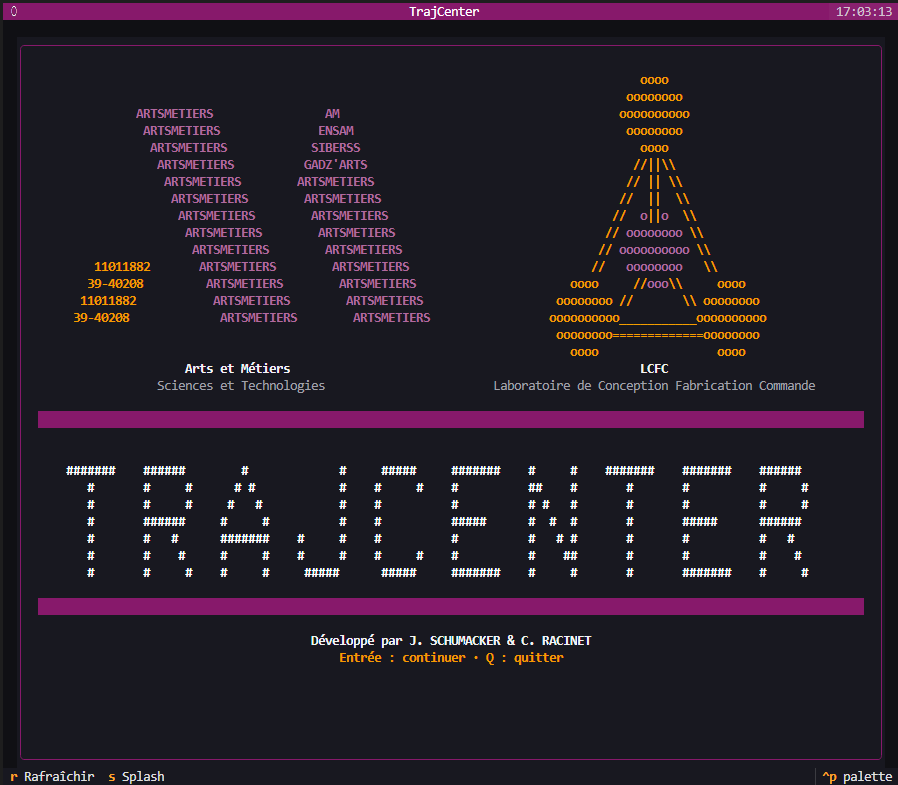
\includegraphics[width=0.5\linewidth]{figures/screenshot/tui_splash.png}
    \caption{Écran d'accueil de TrajCenter}
    \label{fig:pc-tui-splash}
\end{figure}


\subsubsection{Menu principal}
\label{subsubsec:pc-tui-home}

Le menu principal donne accès aux actions suivantes :

\begin{table}[ht]
    \centering
    \begin{tabularx}{\linewidth}{
        |p{0.31\linewidth}
        |X|
    }
        \hline
        \textbf{Action} &
        \textbf{Fonction} \\
        \hline

        Convertir une trajectoire &
        Convertit un fichier CSV, Excel, APT ou RAPID MOD en archive
        \texttt{.trajcenter}. \\
        \hline

        Exporter une trajectoire &
        Exporte une archive \texttt{.trajcenter} en CSV ou en Excel. \\
        \hline

        Explorer le store local &
        Affiche les archives présentes dans le store configuré. \\
        \hline

        Démarrer supervision robot ABB &
        Ouvre l'écran permettant de démarrer et d'arrêter le superviseur
        ABB RWS. Cette action nécessite le support robot. \\
        \hline

        Paramètres &
        Modifie le store et les paramètres de connexion utilisés pendant la
        session courante. \\
        \hline

        Quitter &
        Ferme l'application. \\
        \hline
    \end{tabularx}
    \caption{Actions disponibles depuis le menu principal}
    \label{tab:pc-tui-home-actions}
\end{table}

La partie droite de l'écran présente l'état du store local. Elle affiche :

\begin{itemize}
    \item le chemin du store ;
    \item le nombre d'archives détectées ;
    \item jusqu'à cinq entrées du store, avec leur nom, leur nombre de points
    et leur type de process.
\end{itemize}

Lorsqu'une action est sélectionnée, sa description apparaît dans la partie
inférieure de l'écran.

Si les dépendances ABB ne sont pas installées, l'action de supervision est
désactivée et porte la mention \og option non installée \fg{}. Les opérations
de conversion, d'export et de consultation du store restent disponibles.


\begin{figure}[ht]
    \centering
    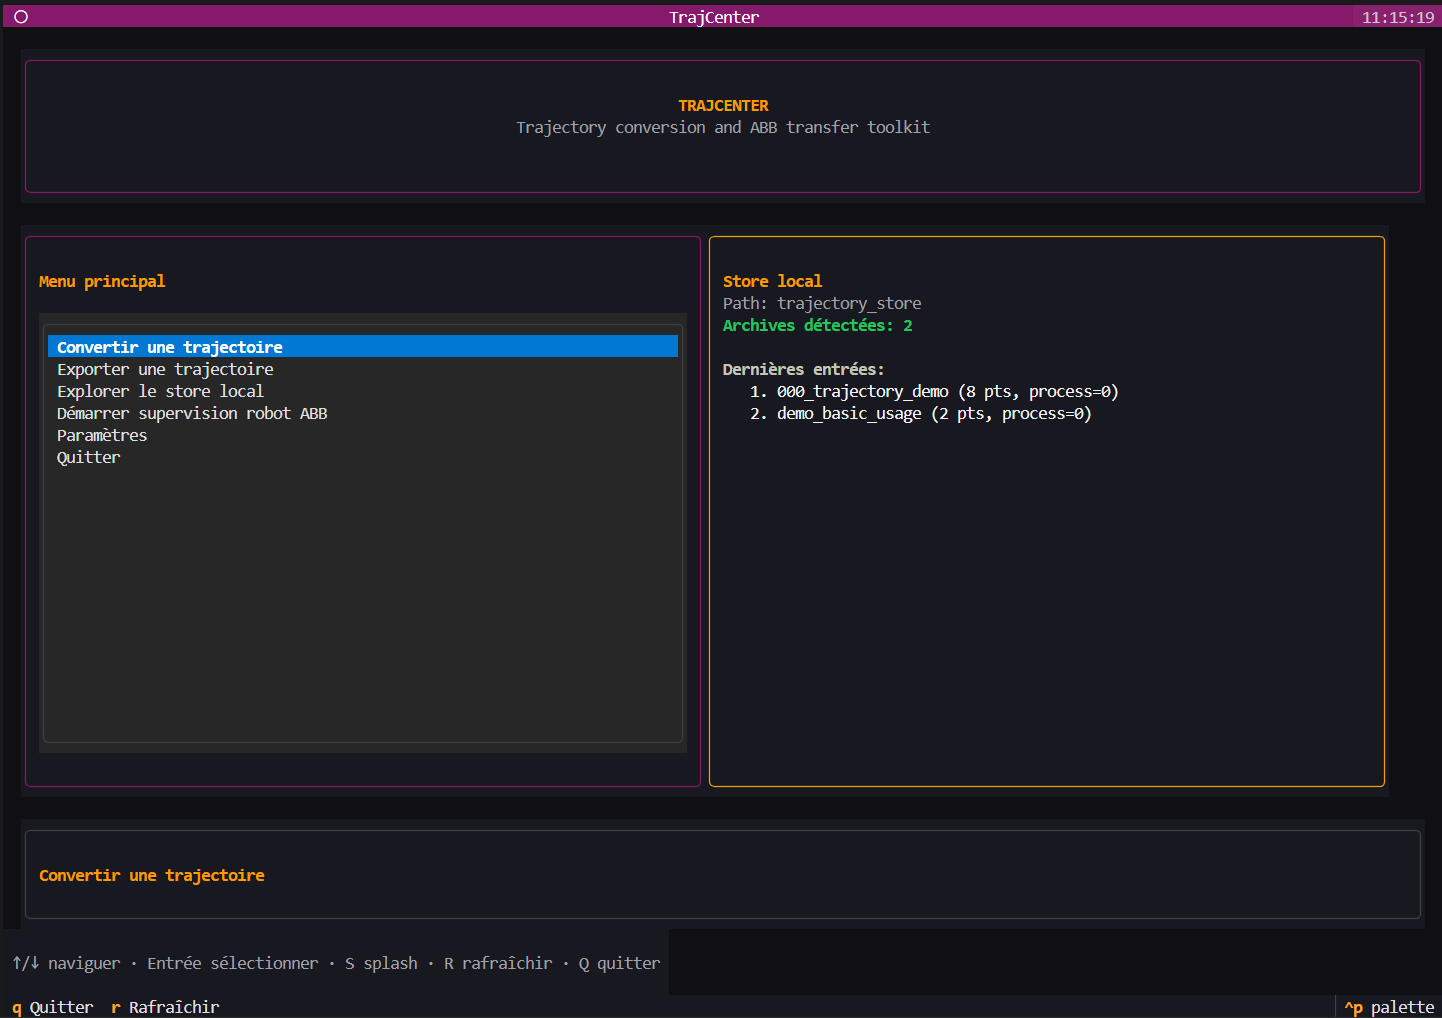
\includegraphics[width=0.5\linewidth]{figures/screenshot/tui_home.png}
    \caption{Menu principal de TrajCenter}
    \label{fig:pc-tui-home}
\end{figure}


\subsubsection{Navigation au clavier}
\label{subsubsec:pc-tui-navigation}

La navigation générale repose sur les touches présentées dans le
tableau~\ref{tab:pc-tui-keyboard}.

\begin{table}[ht]
    \centering
    \begin{tabularx}{\linewidth}{
        |p{0.25\linewidth}
        |X|
    }
        \hline
        \textbf{Touche} &
        \textbf{Action} \\
        \hline

        Flèches &
        Déplacent la sélection dans les menus, les listes et les tableaux. \\
        \hline

        \texttt{Tab} et
        \texttt{Maj+Tab} &
        Déplacent le focus entre les champs et les boutons. \\
        \hline

        \texttt{Entrée} &
        Sélectionne une action, ouvre une liste ou active le bouton ayant le
        focus. \\
        \hline

        \texttt{B} ou
        \texttt{Échap} &
        Revient au menu principal depuis les écrans fonctionnels. Sur l'écran
        initial, \texttt{Échap} ferme l'application. \\
        \hline

        \texttt{R} &
        Réinitialise le formulaire de conversion, d'export ou de paramètres.
        Dans l'écran du store, cette touche recharge la liste des archives. \\
        \hline

        \texttt{S} &
        Affiche l'écran d'accueil depuis le menu principal. \\
        \hline

        \texttt{X} &
        Demande l'arrêt du superviseur depuis l'écran Robot. \\
        \hline

        \texttt{Q} &
        Quitte l'application. \\
        \hline

        \texttt{Ctrl+Shift+V} &
        Colle du texte dans un champ, selon le terminal utilisé. \\
        \hline
    \end{tabularx}
    \caption{Principaux raccourcis de l'interface terminal}
    \label{tab:pc-tui-keyboard}
\end{table}

Les raccourcis réellement actifs sont également rappelés dans le pied de
chaque écran.


\subsubsection{Écran de conversion}
\label{subsubsec:pc-tui-convert-screen}

L'écran de conversion contient les champs suivants :

\begin{table}[ht]
    \centering
    \begin{tabularx}{\linewidth}{
        |p{0.28\linewidth}
        |X|
    }
        \hline
        \textbf{Champ} &
        \textbf{Description} \\
        \hline

        Fichier source &
        Chemin du fichier CSV, Excel, APT, APTSOURCE ou RAPID MOD à
        convertir. Ce champ est obligatoire. \\
        \hline

        Dossier destination &
        Répertoire dans lequel l'archive \texttt{.trajcenter} sera créée. La
        valeur initiale correspond au store configuré. \\
        \hline

        Nom de sortie &
        Nom facultatif de l'archive, sans extension. S'il est vide, le nom du
        fichier source est utilisé. \\
        \hline

        Format source &
        Format imposé par l'utilisateur ou auto-détection à partir de
        l'extension du fichier. \\
        \hline
    \end{tabularx}
    \caption{Champs de l'écran de conversion}
    \label{tab:pc-tui-convert-fields}
\end{table}

Le bouton \og Convertir vers \texttt{.trajcenter} \fg{} lance la conversion.
En cas de succès, l'interface affiche le chemin de l'archive créée. En cas
d'échec, le message transmis par le convertisseur est affiché dans la zone de
statut.

La touche \texttt{R} efface le fichier source et le nom de sortie, restaure le
store comme destination et replace le format sur l'auto-détection.


\begin{figure}[ht]
    \centering
    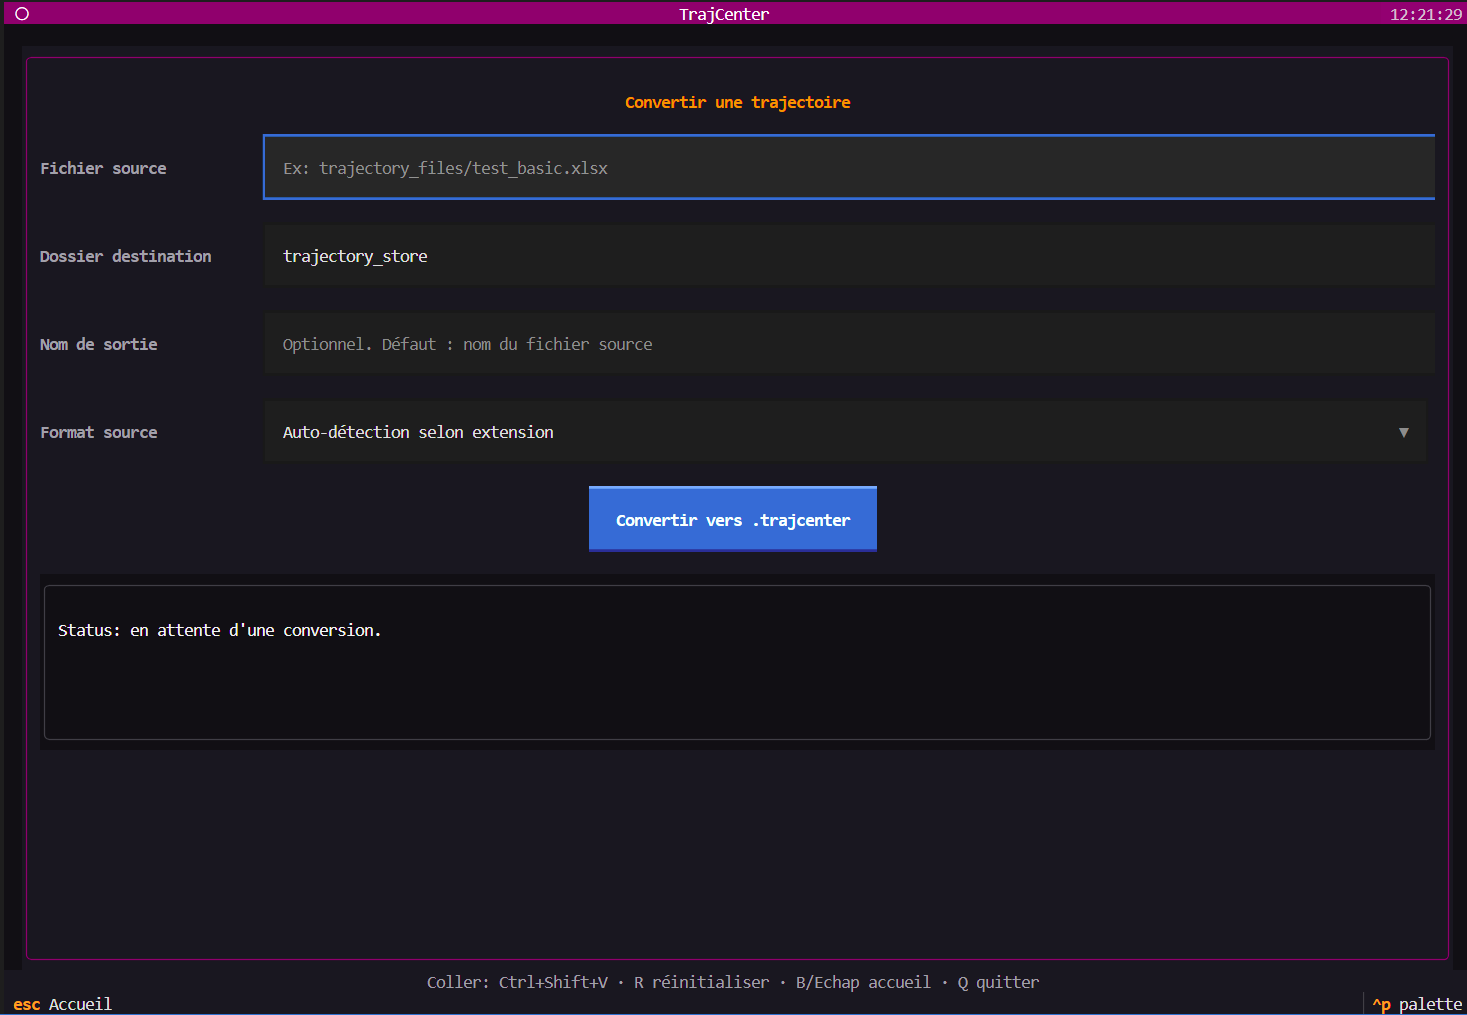
\includegraphics[width=0.5\linewidth]{figures/screenshot/tui_convert.png}
    \caption{Fenêtre de conversion de fichiers}
    \label{fig:pc-tui-convert}
\end{figure}

\subsubsection{Écran d'export}
\label{subsubsec:pc-tui-export-screen}

L'écran d'export contient :

\begin{itemize}
    \item le chemin de l'archive \texttt{.trajcenter} source ;
    \item le dossier destination, initialisé à
    \texttt{trajectory\_exports} ;
    \item le format de sortie, CSV ou Excel.
\end{itemize}

Le format sélectionné par défaut est CSV. Le bouton
\og Exporter la trajectoire \fg{} charge l'archive puis crée le fichier dans
le dossier indiqué.

Après l'opération, la zone de statut affiche soit le chemin du fichier créé,
soit le message d'erreur correspondant.

\begin{figure}[ht]
    \centering
    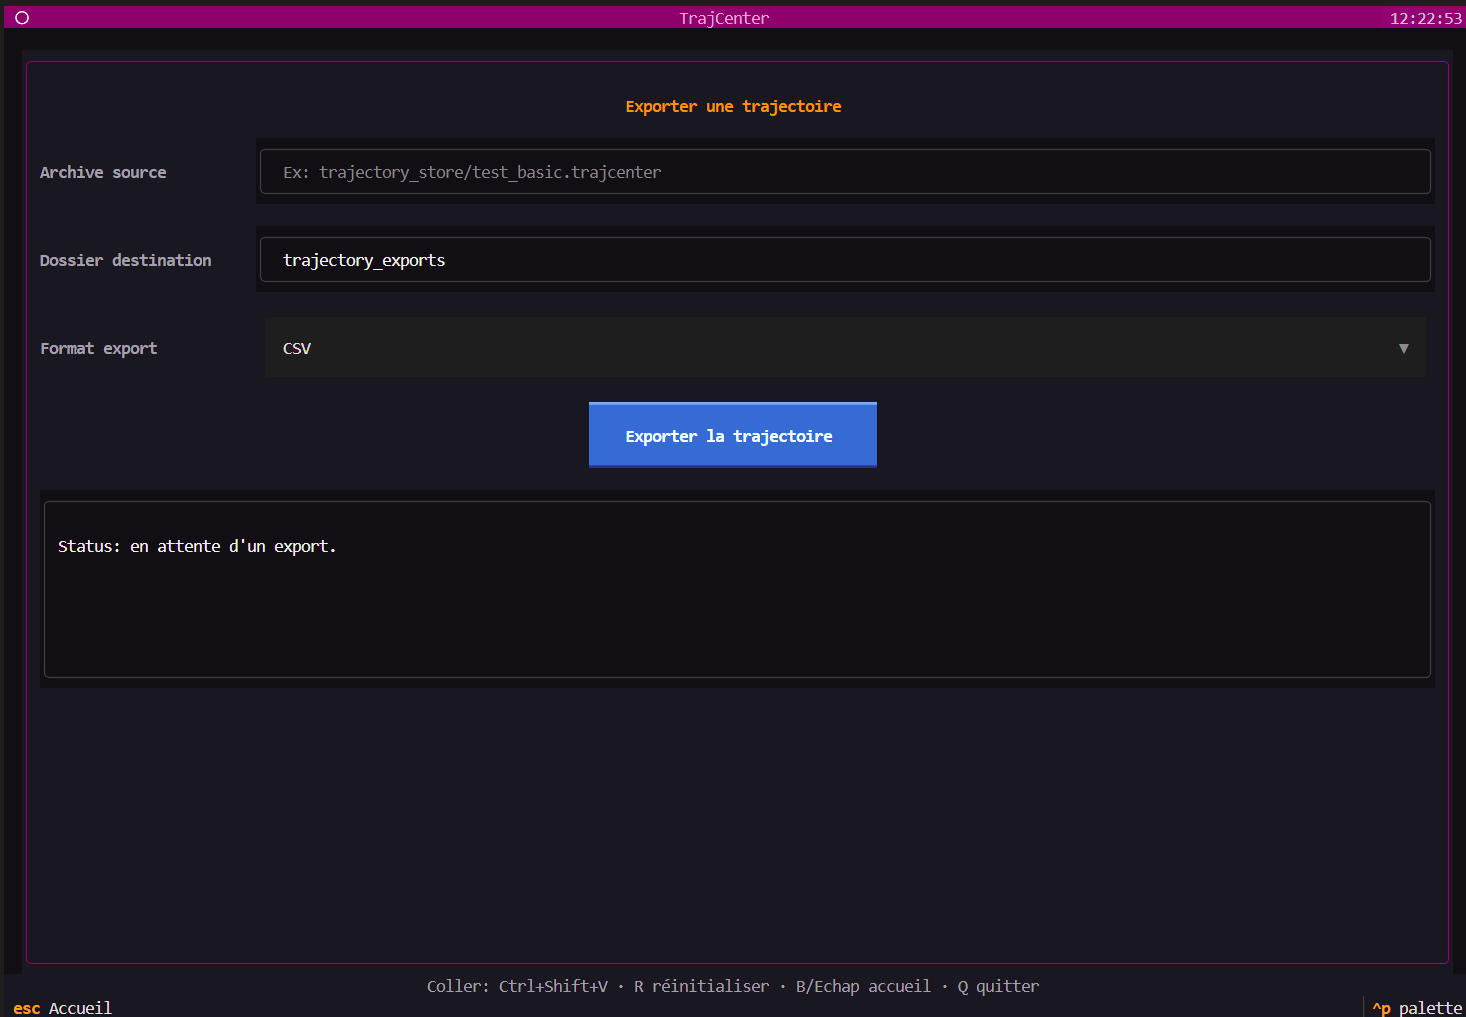
\includegraphics[width=0.5\linewidth]{figures/screenshot/tui_export.png}
    \caption{Écran d'export d'une archive \texttt{.trajcenter}}
    \label{fig:pc-tui-export}
\end{figure}

\subsubsection{Écran du store local}
\label{subsubsec:pc-tui-store-screen}

L'écran \og Store local TrajCenter \fg{} affiche le chemin du store configuré
et une table contenant les colonnes suivantes :

\begin{itemize}
    \item l'index de l'archive ;
    \item le nom de la trajectoire ;
    \item le nombre de points ;
    \item le type de process ;
    \item le nom du fichier.
\end{itemize}

La touche \texttt{R} rescane le répertoire et met la table à jour. La zone de
statut indique le nombre d'archives détectées ou signale une erreur d'accès au
store.

Dans la version actuelle, cet écran permet uniquement de consulter la liste
des archives. L'inspection détaillée d'une archive doit être réalisée avec la
commande \texttt{trajcenter store inspect} décrite dans la
section~\ref{subsec:pc-store}.


\begin{figure}[ht]
    \centering
    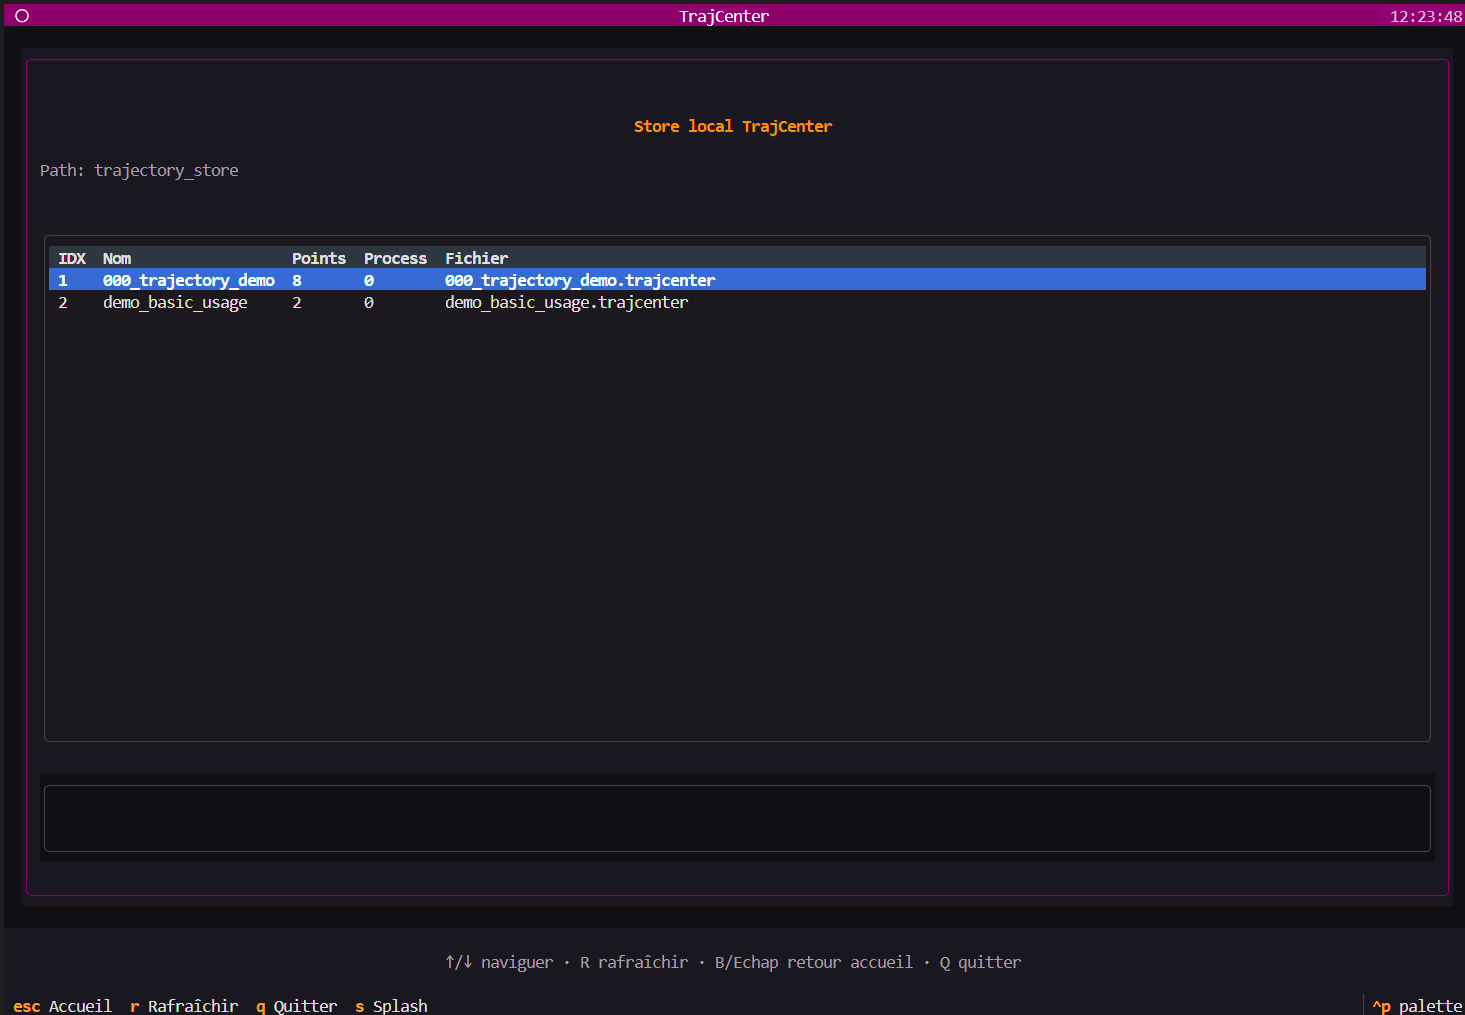
\includegraphics[width=0.5\linewidth]{figures/screenshot/tui_store.png}
    \caption{Consultation des trajectoires disponibles dans le store local}
    \label{fig:pc-tui-store}
\end{figure}

\subsubsection{Écran des paramètres}
\label{subsubsec:pc-tui-settings-screen}

L'écran des paramètres permet de modifier la configuration partagée par les
différents écrans de la TUI.

Les paramètres disponibles sont présentés dans le
tableau~\ref{tab:pc-tui-settings}.

\begin{table}[ht]
    \centering
    \small
    \begin{tabularx}{\linewidth}{
        |p{0.29\linewidth}
        |X|
    }
        \hline
        \textbf{Paramètre} &
        \textbf{Description} \\
        \hline

        Store local &
        Répertoire contenant les archives \texttt{.trajcenter}. \\
        \hline

        Fichier \texttt{.env} &
        Fichier facultatif contenant la configuration RWS. \\
        \hline

        Host robot &
        Adresse IP ou nom d'hôte du contrôleur ABB. \\
        \hline

        Port robot &
        Port HTTP du service RWS. \\
        \hline

        Utilisateur &
        Nom du compte ABB utilisé pour l'authentification. \\
        \hline

        Password env &
        Nom de la variable d'environnement contenant le mot de passe. Le mot
        de passe lui-même n'est pas saisi dans cet écran. \\
        \hline

        Timeout &
        Timeout des requêtes RWS, en secondes. La virgule et le point sont
        acceptés comme séparateur décimal. \\
        \hline

        Task RAPID &
        Tâche contenant le module TrajCenter. La valeur initiale est
        \texttt{T\_ROB1}. \\
        \hline

        Module RAPID &
        Nom du module système. La valeur initiale est
        \texttt{TRAJCENTER}. \\
        \hline

        Mastership retries &
        Nombre de tentatives d'acquisition de la Mastership. La valeur doit être un
        entier supérieur ou égal à \texttt{1}. \\
        \hline

        Log level &
        Niveau de journalisation transmis au superviseur. La valeur initiale
        est \texttt{INFO}. \\
        \hline
    \end{tabularx}
    \caption{Paramètres modifiables depuis la TUI}
    \label{tab:pc-tui-settings}
\end{table}

Le bouton \og Appliquer pour cette session \fg{} valide les champs et met à jour la configuration en mémoire. Ces modifications ne sont pas enregistrées de manière permanente : elles sont perdues à la fermeture de TrajCenter.

Les valeurs définies dans la TUI sont transmises au superviseur pour la session courante. Elles sont donc prioritaires sur les valeurs correspondantes du fichier \texttt{.env}. Avant de démarrer la supervision, l'utilisateur doit vérifier le store, la tâche RAPID, le module RAPID et les paramètres de connexion affichés dans l'interface.

Les valeurs effectivement utilisées sont rappelées dans l'écran de supervision et dans les journaux au démarrage.

La touche \texttt{R} ne restaure pas les valeurs d'installation. Elle recharge dans le formulaire la configuration actuellement appliquée.


\begin{figure}[ht]
    \centering
    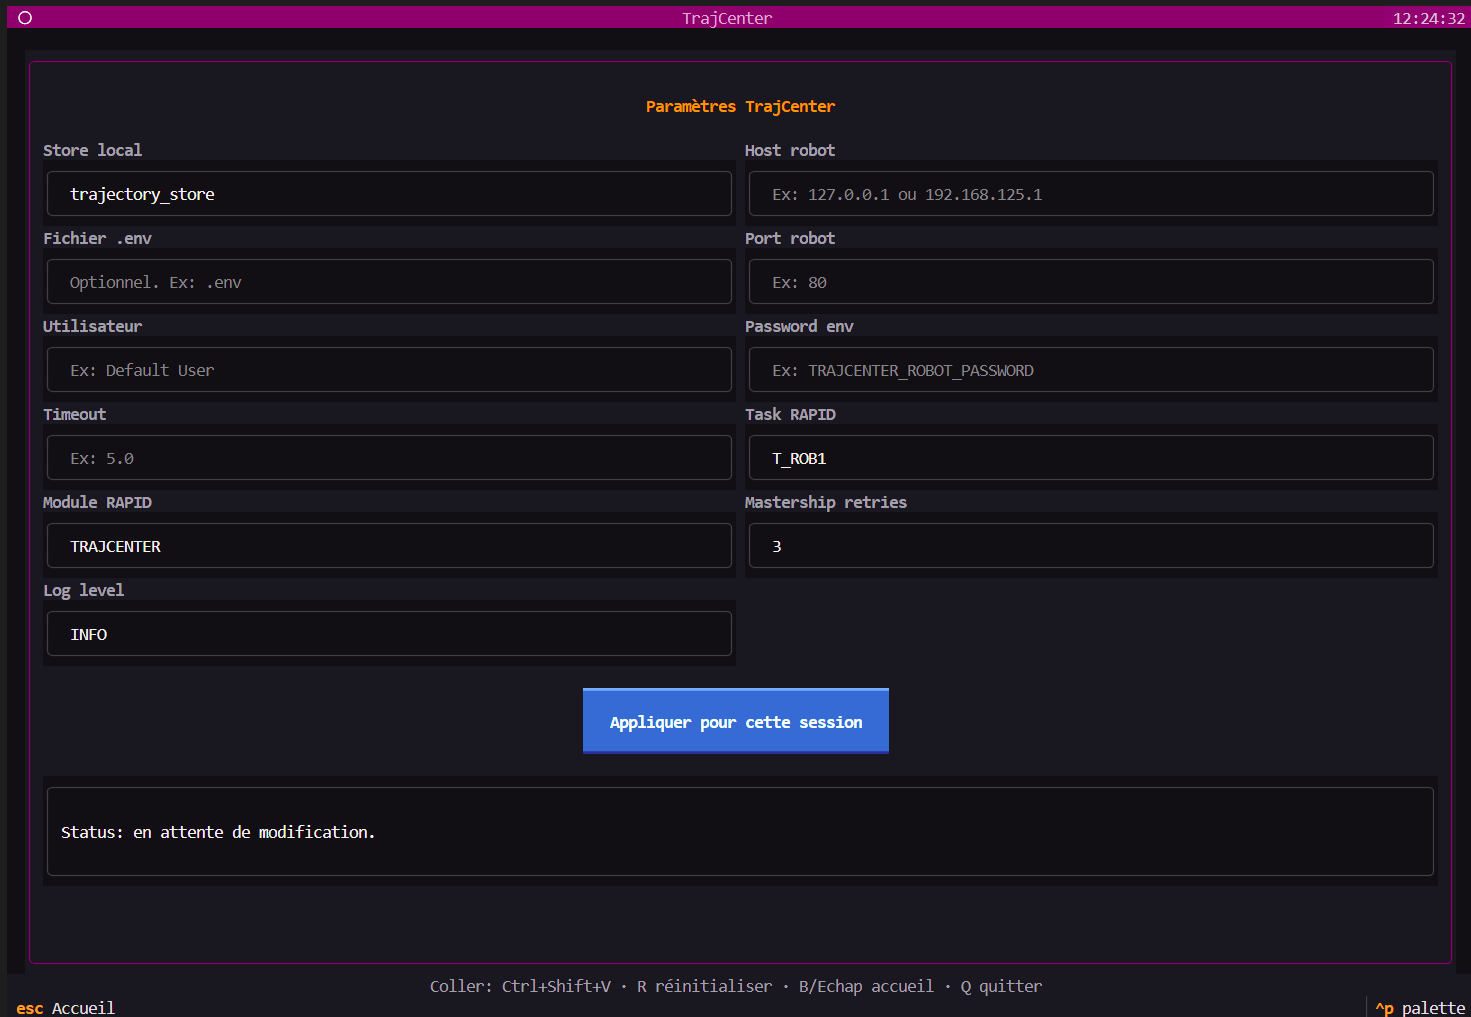
\includegraphics[width=0.5\linewidth]{figures/screenshot/tui_settings.png}
    \caption{Configuration de la session et de la connexion au contrôleur}
    \label{fig:pc-tui-settings}
\end{figure}


\subsubsection{Écran de supervision robot}
\label{subsubsec:pc-tui-robot-screen}

L'écran de supervision n'est accessible que lorsque le support ABB est
disponible dans l'environnement courant.

Il affiche :

\begin{itemize}
    \item le chemin du store local ;
    \item la tâche RAPID utilisée ;
    \item le nom du module RAPID ;
    \item l'état du superviseur ;
    \item les journaux produits par le superviseur.
\end{itemize}

Le bouton \og Démarrer la supervision \fg{} lance le superviseur ABB dans un
processus séparé. Les sorties standard et les erreurs sont affichées en temps
réel dans la zone de journalisation.

Lorsque le superviseur est actif, le bouton devient
\og Arrêter la supervision \fg{}. L'arrêt peut également être demandé avec la
touche \texttt{X}.

Il n'est pas possible de revenir au menu principal pendant que le processus
est actif. Il faut d'abord demander son arrêt. Si le processus ne répond pas
dans le délai prévu, TrajCenter tente de le terminer de force.

Le code de retour du processus est affiché à la fin de la supervision. Un code
nul indique une terminaison normale ; un code non nul signale une erreur.

\begin{figure}[ht]
    \centering
    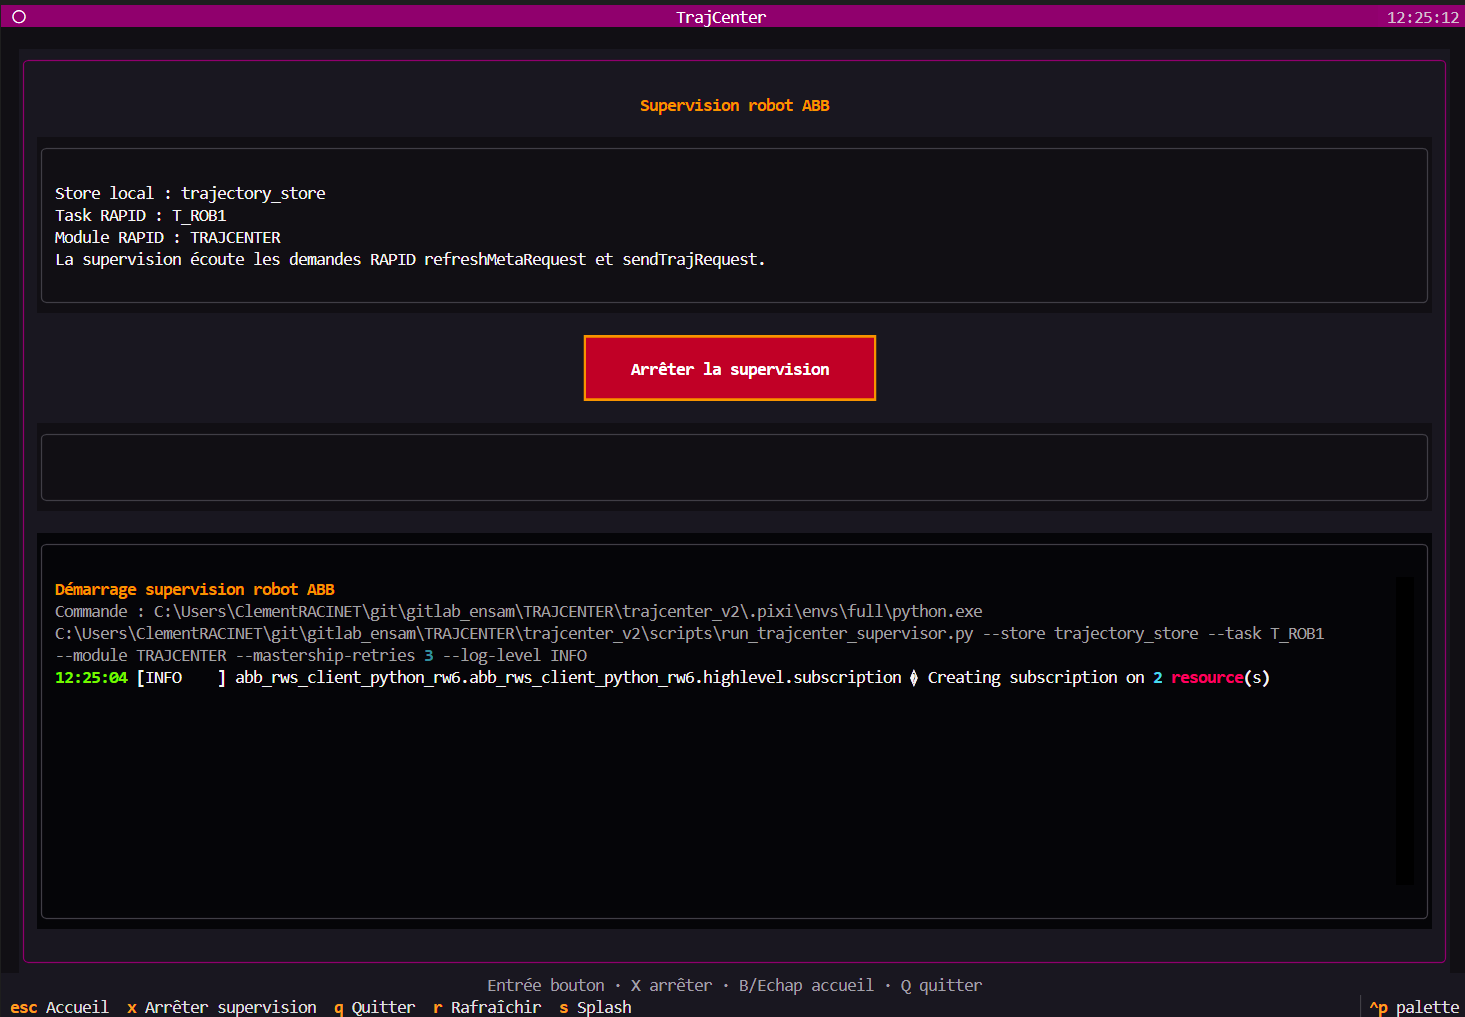
\includegraphics[width=0.5\linewidth]{figures/screenshot/tui_robot.png}
    \caption{Supervision de la connexion au robot et affichage des journaux}
    \label{fig:pc-tui-robot}
\end{figure}

\FloatBarrier

\subsection{Référence de la ligne de commande}
\label{subsec:pc-cli}


Le CLI permet d'exécuter les fonctions de TrajCenter sans ouvrir l'interface Textual. Il convient notamment aux scripts, aux traitements automatisés et aux postes utilisés sans interaction graphique. Les procédures détaillées de conversion, de gestion du store, d'export et de supervision sont décrites dans les sections précédentes. Cette section fournit uniquement une vue d'ensemble des commandes disponibles.

Pour connaître toutes les options d'une commande, utiliser
\texttt{--help}. Par exemple :

\begin{lstlisting}[
    language=bash,
    caption={Affichage des options du superviseur},
    label={lst:pc-cli-supervisor-help}
]
pixi run -e full trajcenter robot supervise --help
\end{lstlisting}


La syntaxe générale est :

\begin{lstlisting}[
    language=bash,
    caption={Syntaxe générale du CLI TrajCenter},
    label={lst:pc-cli-general-syntax}
]
pixi run -e <environnement> trajcenter <commande> [options]
\end{lstlisting}

L'environnement peut être \texttt{default}, \texttt{tui}, \texttt{robot} ou
\texttt{full}, selon les fonctionnalités nécessaires.

Pour afficher l'aide générale :

\begin{lstlisting}[
    language=bash,
    caption={Affichage de l'aide générale},
    label={lst:pc-cli-help}
]
pixi run -e tui trajcenter --help
\end{lstlisting}

Pour afficher l'aide d'une commande particulière :

\begin{lstlisting}[
    language=bash,
    caption={Affichage de l'aide d'une commande},
    label={lst:pc-cli-command-help}
]
pixi run -e tui trajcenter convert --help
\end{lstlisting}

Les commandes disponibles sont résumées dans le
tableau~\ref{tab:pc-cli-commands}.

\begin{table}[ht]
    \centering
    \small
    \begin{tabularx}{\linewidth}{
        |p{0.33\linewidth}
        |X|
    }
        \hline
        \textbf{Commande} &
        \textbf{Fonction} \\
        \hline

        \texttt{trajcenter version} &
        Affiche la version installée de TrajCenter. \\
        \hline

        \texttt{trajcenter convert} &
        Convertit un fichier source en archive
        \texttt{.trajcenter}. \\
        \hline

        \texttt{trajcenter export} &
        Exporte une archive en CSV ou en Excel. \\
        \hline

        \texttt{trajcenter tui} &
        Lance l'interface Textual avec un store configurable. \\
        \hline

        \texttt{trajcenter store list} &
        Liste les archives du store local. \\
        \hline

        \texttt{trajcenter store inspect} &
        Affiche les informations détaillées d'une archive sélectionnée par
        son nom, son fichier, son nom sans extension ou son index. \\
        \hline

        \texttt{trajcenter robot check} &
        Vérifie que le support logiciel ABB est disponible. Cette commande ne
        teste pas la connexion au contrôleur. \\
        \hline

        \texttt{trajcenter robot supervise} &
        Lance la boucle de supervision ABB RWS. \\
        \hline
    \end{tabularx}
    \caption{Commandes principales du CLI TrajCenter}
    \label{tab:pc-cli-commands}
\end{table}


Lorsqu'une commande de conversion ou d'export réussit, le CLI affiche le chemin du fichier créé. Lorsqu'une erreur attendue survient, il affiche un message commençant par \texttt{Error:} et retourne un code d'échec.

Les sous-commandes \texttt{store} et \texttt{robot} doivent obligatoirement être complétées par une action. En cas d'oubli, le CLI indique la commande d'aide correspondante.

%------------------------------------------------------------------------------
% Partie : Utilisation côté RAPID
%------------------------------------------------------------------------------
\section{Utilisation côté RAPID}
\label{sec:rapid-usage}

Cette section présente l'utilisation de TrajCenter depuis un programme RAPID.
Elle s'adresse aux roboticiens et automaticiens chargés d'installer le module
système, de configurer la cellule, de demander une trajectoire et d'exécuter
les données transférées.

Le programme RAPID ne lit jamais directement une archive
\texttt{.trajcenter}. Il émet une requête dans le contrôleur, attend son
traitement par le superviseur Python, puis utilise le payload publié dans le
module système \texttt{TRAJCENTER}.

Les responsabilités sont réparties de la manière suivante :

\begin{itemize}
    \item le \textbf{programme RAPID utilisateur} sélectionne les trajectoires,
    contrôle les états et déclenche l'exécution ;
    \item le \textbf{superviseur Python} lit le store local, valide l'archive,
    contrôle sa cohérence avec le catalogue, résout les noms de tools et de
    workobjects, puis transfère le payload avec ABB Robot Web Services ;
    \item le \textbf{module système \texttt{TRAJCENTER}} fournit les variables
    d'échange, les routines publiques, les interfaces process et le moteur
    commun de mouvement.
\end{itemize}

Dans une utilisation normale, le programme RAPID suit cette séquence :

\begin{enumerate}
    \item initialiser les erreurs locales TrajCenter ;
    \item initialiser et compléter la configuration de cellule ;
    \item définir les valeurs par défaut autorisées ;
    \item demander le rafraîchissement du catalogue des trajectoires ;
    \item demander une trajectoire par son nom ou son index ;
    \item attendre la publication complète du payload ;
    \item contrôler les données et le type de process chargés ;
    \item effectuer les contrôles de sécurité propres à la cellule ;
    \item exécuter la trajectoire avec
    \texttt{TRAJCENTER\_ExecuteLoaded}.
\end{enumerate}

Toutes les trajectoires utilisent la même API d'exécution. Une trajectoire sans
process correspond au cas où \texttt{loadedProcessType} vaut
\texttt{processNone}.


%==============================================================================
\subsection{Installation et principe de fonctionnement}
\label{subsec:rapid-installation-operation}
%==============================================================================

Cette première étape consiste à charger le module système dans la bonne tâche
RAPID et à vérifier que le programme utilisateur peut accéder à son API.


\subsubsection{Installation du module sur le contrôleur}
\label{subsubsec:rapid-module-installation}

Le fichier \texttt{TRAJCENTER.sys} doit être chargé comme module système dans
la tâche RAPID utilisée par TrajCenter, généralement \texttt{T\_ROB1}.

L'installation peut être réalisée depuis RobotStudio ou depuis l'interface de
gestion des modules du contrôleur. Après le chargement, vérifier que :

\begin{itemize}
    \item le module apparaît sous le nom \texttt{TRAJCENTER} ;
    \item il est chargé comme module système ;
    \item il se trouve dans la tâche configurée côté PC ;
    \item aucune erreur de syntaxe ou de chargement RAPID n'est signalée ;
    \item sa version est compatible avec celle du superviseur Python.
\end{itemize}

La tâche et le nom du module doivent correspondre aux valeurs configurées sur
le PC :

\begin{lstlisting}[
    language={},
    caption={Correspondance entre la configuration PC et le module RAPID},
    label={lst:rapid-pc-module-correspondence}
]
TRAJCENTER_RWS_TASK=T_ROB1
TRAJCENTER_RWS_MODULE=TRAJCENTER
\end{lstlisting}

Si le superviseur cible \texttt{T\_ROB1} et le module
\texttt{TRAJCENTER}, les symboles utilisés pour les échanges RWS doivent être
accessibles dans cette tâche et dans ce module.

Le module peut rester chargé lorsque le superviseur Python est arrêté. En
revanche, aucune nouvelle demande de rafraîchissement ou de transfert ne peut
aboutir sans superviseur actif.


\subsubsection{Principe d'une requête RAPID}
\label{subsubsec:rapid-request-principle}

Une requête RAPID n'est pas un appel direct à une fonction Python. Le programme
modifie une variable persistante du module système. Le superviseur, abonné aux
variables concernées par RWS, détecte le changement et effectue le traitement
demandé.

Deux requêtes principales sont utilisées :

\begin{table}[ht]
    \centering
    \begin{tabularx}{\linewidth}{
        |p{0.27\linewidth}
        |p{0.25\linewidth}
        |X|
    }
        \hline
        \textbf{Requête} &
        \textbf{Variable RAPID} &
        \textbf{Résultat attendu} \\
        \hline

        Rafraîchissement du catalogue &
        \texttt{refreshMetaRequest} &
        Mise à jour de \texttt{nbTrajAvailable} et du tableau
        \texttt{trajectories}. \\
        \hline

        Chargement d'une trajectoire &
        \texttt{sendTrajRequest} &
        Validation, résolution et publication du nouveau payload dans
        \texttt{trajData}, \texttt{processParams},
        \texttt{loadedProcessType} et
        \texttt{nbLoadedTrajPoints}. \\
        \hline
    \end{tabularx}
    \caption{Principales requêtes échangées avec le superviseur}
    \label{tab:rapid-main-requests}
\end{table}

Le programme utilisateur ne doit normalement pas modifier directement ces
variables. Il doit utiliser les routines publiques
\texttt{TRAJCENTER\_*}, qui réalisent les contrôles et les réinitialisations
nécessaires.


\subsubsection{Conditions nécessaires au fonctionnement}
\label{subsubsec:rapid-operation-prerequisites}

Une demande de transfert nécessite simultanément :

\begin{itemize}
    \item le module \texttt{TRAJCENTER.sys} chargé dans la bonne tâche ;
    \item un superviseur TrajCenter actif sur le PC ;
    \item une connexion réseau fonctionnelle ;
    \item ABB Robot Web Services accessible ;
    \item un compte autorisé à lire et écrire les données RAPID ;
    \item la possibilité pour le superviseur d'acquérir la Mastership ;
    \item un store local accessible contenant au moins une archive valide ;
    \item un catalogue process cohérent avec les capacités réellement
    implémentées dans le module RAPID.
\end{itemize}

Si le superviseur est arrêté ou si la connexion est interrompue, la requête
RAPID peut rester active jusqu'à l'expiration du délai d'attente.


%==============================================================================
\subsection{Configuration de la cellule}
\label{subsec:rapid-cell-configuration}
%==============================================================================

La configuration de la cellule indique au superviseur quels tools et
workobjects peuvent être utilisés. Elle définit également les valeurs par
défaut autorisées lorsque certaines informations sont absentes d'une
trajectoire.


\subsubsection{Initialisation de l'API}
\label{subsubsec:rapid-api-initialization}

Avant d'appeler une routine TrajCenter susceptible de lever une erreur RAPID
locale, le programme doit initialiser les numéros d'erreur utilisés par l'API.

L'initialisation minimale est la suivante :

\begin{lstlisting}[
    style=rapid,
    caption={Initialisation de l'API TrajCenter},
    label={lst:rapid-initialization}
]
TRAJCENTER_InitErrors;
TRAJCENTER_InitCellConfig;
\end{lstlisting}

La routine \texttt{TRAJCENTER\_InitErrors} initialise les erreurs locales
TrajCenter. Elle peut être appelée plusieurs fois.

La routine \texttt{TRAJCENTER\_InitCellConfig} ajoute ou met à jour la
configuration minimale contenant :

\begin{itemize}
    \item le tool \texttt{tool0} ;
    \item le workobject \texttt{wobj0}.
\end{itemize}

Cette routine ne vide pas les tools et workobjects déjà enregistrés. Elle
appelle cependant les routines d'ajout ou de mise à jour, ce qui invalide le
payload éventuellement chargé.

L'initialisation doit donc généralement être réalisée au démarrage du programme
utilisateur, avant le premier chargement d'une trajectoire. Elle ne doit pas
être répétée entre le chargement et l'exécution.


\subsubsection{Déclaration des tools et des workobjects}
\label{subsubsec:rapid-tools-wobjs}

Les archives \texttt{.trajcenter} utilisent des noms logiques de tools et de
workobjects, par exemple \texttt{productionTool} ou
\texttt{productionWobj}. Leur définition géométrique reste maîtrisée par la
cellule robotisée.

Lors du transfert, le superviseur recherche les noms demandés dans les tableaux
RAPID \texttt{trajTools} et \texttt{trajWobjs}. Il associe ensuite les points
aux entrées correspondantes en écrivant des index base~1 dans
\texttt{trajData}.

Un tool et un workobject peuvent être exposés à TrajCenter avec les routines
\texttt{TRAJCENTER\_UpsertTool} et
\texttt{TRAJCENTER\_UpsertWobj} :

\begin{lstlisting}[
    style=rapid,
    caption={Déclaration d'un tool et d'un workobject},
    label={lst:rapid-tool-wobj-configuration}
]
PERS tooldata productionTool := [
    TRUE,
    [[0, 0, 0], [1, 0, 0, 0]],
    [1, [0, 0, 50], [1, 0, 0, 0],
     0.01, 0.01, 0.01]
];

PERS wobjdata productionWobj := [
    FALSE,
    TRUE,
    "",
    [[0, 0, 0], [1, 0, 0, 0]],
    [[0, 0, 0], [1, 0, 0, 0]]
];

PROC ConfigureTrajCenterCell()

    TRAJCENTER_UpsertTool
        "productionTool",
        productionTool;

    TRAJCENTER_UpsertWobj
        "productionWobj",
        productionWobj;

ENDPROC
\end{lstlisting}

Le premier argument est le nom logique utilisé dans les trajectoires. Le
second argument est la donnée RAPID réellement utilisée par le robot.

Si le nom existe déjà, la valeur associée est remplacée. Sinon, la routine
utilise le premier emplacement libre.

Les noms doivent correspondre exactement à ceux des archives. La comparaison
réalisée par le module est une comparaison directe des chaînes.

Toute opération d'ajout ou de mise à jour invalide le payload chargé, y compris
lorsque le nom existait déjà. Une trajectoire doit donc être redemandée après
une modification de la configuration.


\subsubsection{Maintenance des tools et des workobjects}
\label{subsubsec:rapid-tools-wobjs-maintenance}

Les principales routines de maintenance sont présentées dans le
tableau~\ref{tab:rapid-cell-config-routines}.

\begin{table}[ht]
    \centering
    \begin{tabularx}{\linewidth}{
        |p{0.37\linewidth}
        |X|
    }
        \hline
        \textbf{Routine} &
        \textbf{Utilisation} \\
        \hline

        \texttt{TRAJCENTER\_UpsertTool} &
        Ajoute un tool ou remplace sa valeur s'il existe déjà. \\
        \hline

        \texttt{TRAJCENTER\_UpsertWobj} &
        Ajoute un workobject ou remplace sa valeur s'il existe déjà. \\
        \hline

        \texttt{TRAJCENTER\_DeleteTool} &
        Supprime un tool exposé à TrajCenter. \\
        \hline

        \texttt{TRAJCENTER\_DeleteWobj} &
        Supprime un workobject exposé à TrajCenter. \\
        \hline

        \texttt{TRAJCENTER\_ClearTools} &
        Vide le tableau des tools exposés. \\
        \hline

        \texttt{TRAJCENTER\_ClearWobjs} &
        Vide le tableau des workobjects exposés. \\
        \hline

        \texttt{TRAJCENTER\_ClearCellConfig} &
        Vide les tableaux de tools et de workobjects. \\
        \hline
    \end{tabularx}
    \caption{Routines de configuration de la cellule}
    \label{tab:rapid-cell-config-routines}
\end{table}

Toutes ces opérations invalident la trajectoire actuellement chargée. Les
points transférés contiennent en effet des index associés à la configuration
présente au moment du transfert.

Après une modification, appliquer la séquence suivante :

\begin{enumerate}
    \item mettre à jour le tool ou le workobject ;
    \item redemander la trajectoire ;
    \item attendre la fin du nouveau transfert ;
    \item vérifier que \texttt{trajReady} vaut \texttt{TRUE} ;
    \item vérifier \texttt{nbLoadedTrajPoints} ;
    \item vérifier \texttt{loadedProcessType} ;
    \item reprendre l'exécution uniquement après les contrôles de sécurité.
\end{enumerate}

Après un appel à \texttt{TRAJCENTER\_ClearCellConfig}, il est recommandé
d'appeler \texttt{TRAJCENTER\_InitCellConfig} afin de recréer au minimum
\texttt{tool0} et \texttt{wobj0}.

Les routines de suppression et de vidage sont destinées à la mise en service
ou à la maintenance. Elles ne doivent pas être appelées pendant l'exécution
d'une trajectoire.


\subsubsection{Configuration des valeurs par défaut}
\label{subsubsec:rapid-default-values}

Une trajectoire peut omettre certaines données, notamment la vitesse TCP, la
zone, le tool ou le workobject. Le superviseur n'utilise une valeur par défaut
que lorsque le robot l'autorise explicitement.

Chaque valeur optionnelle est associée à un indicateur
\texttt{hasDefault*}. L'exemple suivant configure les valeurs par défaut de la
cellule :

\begin{lstlisting}[
    style=rapid,
    caption={Configuration des valeurs par défaut robot},
    label={lst:rapid-default-configuration}
]
hasDefaultTcpSpeed := TRUE;
defaultTcpSpeed := 100;

hasDefaultZoneType := TRUE;
defaultZoneType := 255;

hasDefaultToolName := TRUE;
defaultToolName := "productionTool";

hasDefaultWobjName := TRUE;
defaultWobjName := "productionWobj";

defaultMoveType := moveTypeL;
defaultReadConfs := TRUE;
\end{lstlisting}

Dans cet exemple :

\begin{itemize}
    \item la vitesse TCP par défaut est de \texttt{100}~mm/s ;
    \item la zone \texttt{255} est interprétée comme \texttt{fine} ;
    \item le mouvement par défaut est un mouvement linéaire ;
    \item la lecture des configurations d'axes est activée ;
    \item les noms \texttt{productionTool} et
    \texttt{productionWobj} doivent exister dans les tableaux de la cellule.
\end{itemize}

Les valeurs par défaut ne remplacent pas systématiquement les données de la
trajectoire. Elles sont utilisées uniquement lorsque la donnée correspondante
est absente.

Si une donnée nécessaire est absente et qu'aucune valeur par défaut n'est
autorisée, le superviseur refuse le transfert et renseigne les variables de
diagnostic.


\subsubsection{Routine de configuration recommandée}
\label{subsubsec:rapid-config-maintenance}

Il est recommandé de centraliser la configuration TrajCenter dans une routine
dédiée du programme de cellule :

\begin{lstlisting}[
    style=rapid,
    caption={Organisation recommandée de la configuration},
    label={lst:rapid-recommended-cell-configuration}
]
PROC ConfigureTrajCenter()

    TRAJCENTER_InitErrors;
    TRAJCENTER_InitCellConfig;

    TRAJCENTER_UpsertTool
        "productionTool",
        productionTool;

    TRAJCENTER_UpsertWobj
        "productionWobj",
        productionWobj;

    hasDefaultTcpSpeed := TRUE;
    defaultTcpSpeed := 100;

    hasDefaultZoneType := TRUE;
    defaultZoneType := 255;

    hasDefaultToolName := TRUE;
    defaultToolName := "productionTool";

    hasDefaultWobjName := TRUE;
    defaultWobjName := "productionWobj";

    defaultMoveType := moveTypeL;
    defaultReadConfs := TRUE;

ENDPROC
\end{lstlisting}

Cette organisation sépare la configuration de la cellule du cycle de
production. Elle facilite également la vérification des noms et des valeurs
utilisés pendant la mise en service.

Cette routine doit être exécutée avant le chargement de la trajectoire. Les
appels à \texttt{TRAJCENTER\_InitCellConfig},
\texttt{TRAJCENTER\_UpsertTool} et
\texttt{TRAJCENTER\_UpsertWobj} invalident le payload courant.


%==============================================================================
\subsection{Chargement d'une trajectoire}
\label{subsec:rapid-trajectory-loading}
%==============================================================================

Le chargement comporte deux opérations distinctes :

\begin{enumerate}
    \item rafraîchir le catalogue des trajectoires disponibles ;
    \item demander le transfert de la trajectoire sélectionnée.
\end{enumerate}


\subsubsection{Rafraîchissement des métadonnées}
\label{subsubsec:rapid-metadata-refresh}

Avant de sélectionner une trajectoire, le robot doit connaître le contenu du
store local côté PC.

La routine \texttt{TRAJCENTER\_RequestMetaRefresh} active la demande de
rafraîchissement. Le superviseur inspecte alors le store local et met à jour :

\begin{itemize}
    \item \texttt{nbTrajAvailable}, qui contient le nombre de trajectoires
    disponibles ;
    \item \texttt{trajectories}, qui contient leurs métadonnées.
\end{itemize}

Le programme doit attendre la fin de l'opération avec
\texttt{TRAJCENTER\_WaitRequestDone} :

\begin{lstlisting}[
    style=rapid,
    caption={Rafraîchissement du catalogue des trajectoires},
    label={lst:rapid-metadata-refresh}
]
TRAJCENTER_RequestMetaRefresh;
TRAJCENTER_WaitRequestDone 30;

IF transferError = TRUE THEN
    TPWrite "Metadata refresh failed";
    TPWrite "Code:" \Num:=lastErrorCode;
    TPWrite lastError;
    Stop;
ENDIF
\end{lstlisting}

L'argument \texttt{30} correspond ici au délai maximal d'attente, en secondes.

Après un rafraîchissement réussi, seules les entrées suivantes sont valides :

\begin{lstlisting}[
    style=rapid,
    caption={Bornes valides du catalogue},
    label={lst:rapid-valid-metadata-range}
]
trajectories{1}
...
trajectories{nbTrajAvailable}
\end{lstlisting}

Les entrées situées au-delà de \texttt{nbTrajAvailable} doivent être ignorées.
Elles peuvent encore contenir des données provenant d'un rafraîchissement
précédent.

La routine \texttt{TRAJCENTER\_WaitRequestDone} retourne normalement lorsque
\texttt{transferError} devient \texttt{TRUE}. Le programme appelant doit donc
toujours contrôler ce flag après l'attente.

Le rafraîchissement des métadonnées n'invalide pas le payload déjà chargé. Une
trajectoire précédemment publiée peut donc rester valide pendant un simple
rafraîchissement du catalogue.


\subsubsection{Sélection par nom}
\label{subsubsec:rapid-trajectory-selection}

La sélection par nom est recommandée dans les programmes de production. Elle
est généralement plus lisible et plus stable qu'une sélection par index.

L'exemple suivant demande une trajectoire nommée
\texttt{000\_trajectory\_demo} :

\begin{lstlisting}[
    style=rapid,
    caption={Chargement d'une trajectoire par nom},
    label={lst:rapid-load-by-name}
]
TRAJCENTER_RequestTrajByName "000_trajectory_demo";
TRAJCENTER_WaitTrajectoryReady 120;
\end{lstlisting}

Le nom demandé doit correspondre exactement au nom présent dans les
métadonnées. Il peut être différent du nom du fichier
\texttt{.trajcenter}.

La routine \texttt{TRAJCENTER\_RequestTrajByName} :

\begin{enumerate}
    \item recherche le nom avec
    \texttt{TRAJCENTER\_FindTrajectoryIndex} ;
    \item lève \texttt{ERR\_TRAJCENTER\_TRAJ\_NOT\_FOUND} si le nom est
    absent ;
    \item appelle \texttt{TRAJCENTER\_RequestTrajectory} avec l'index trouvé.
\end{enumerate}


\subsubsection{Sélection par index}
\label{subsubsec:rapid-trajectory-selection-index}

Une trajectoire peut également être demandée à partir de son index :

\begin{lstlisting}[
    style=rapid,
    caption={Chargement d'une trajectoire par index},
    label={lst:rapid-load-by-index}
]
TRAJCENTER_RequestTrajectory 1;
TRAJCENTER_WaitTrajectoryReady 120;
\end{lstlisting}

L'index doit être compris entre \texttt{1} et
\texttt{nbTrajAvailable}.

L'ordre du catalogue peut évoluer lorsque le contenu du store change. La
sélection par index convient donc surtout à une interface opérateur affichant
le catalogue courant ou à une utilisation contrôlée après rafraîchissement.


\subsubsection{Invalidation du payload précédent}
\label{subsubsec:rapid-payload-invalidation}

La routine \texttt{TRAJCENTER\_RequestTrajectory} invalide immédiatement le
payload précédent avant d'activer la nouvelle requête.

L'état d'invalidation est le suivant :

\begin{lstlisting}[
    style=rapid,
    caption={Invalidation précédant une nouvelle demande},
    label={lst:rapid-request-invalidation}
]
trajReady := FALSE;
nbLoadedTrajPoints := 0;
loadedProcessType := processNone;
\end{lstlisting}

Les anciennes valeurs de \texttt{trajData} et de
\texttt{processParams} ne sont pas nécessairement effacées. Elles ne sont
cependant plus exploitables, car le payload n'est plus déclaré valide.

Le programme utilisateur ne doit donc jamais utiliser les valeurs résiduelles
des tableaux lorsque \texttt{trajReady} vaut \texttt{FALSE}.


\subsubsection{Publication du nouveau payload}
\label{subsubsec:rapid-payload-publication}

Après réception de la requête, le superviseur charge l'archive sélectionnée,
vérifie sa cohérence avec les métadonnées publiées, lit le contexte robot puis
résout les données dépendantes de la cellule.

Le transfert est ensuite réalisé en trois phases :

\begin{enumerate}
    \item \textbf{invalidation} du payload précédent ;
    \item \textbf{écriture} de \texttt{processParams}, \texttt{trajData},
    \texttt{loadedProcessType} et \texttt{nbLoadedTrajPoints} ;
    \item \textbf{publication} avec \texttt{trajReady} à \texttt{TRUE}, puis
    remise de \texttt{sendTrajRequest} à \texttt{FALSE}.
\end{enumerate}

Le type de process n'est donc pas choisi manuellement par le programme
utilisateur. Il est fourni par l'archive chargée, validé par Python puis écrit
dans \texttt{loadedProcessType}.


\subsubsection{Attente de la fin du transfert}
\label{subsubsec:rapid-synchronization}

La demande de trajectoire est asynchrone. Le programme doit attendre avec :

\begin{lstlisting}[
    style=rapid,
    caption={Attente de la fin d'un transfert},
    label={lst:rapid-wait-trajectory-ready}
]
TRAJCENTER_WaitTrajectoryReady 120;
\end{lstlisting}

Lorsque cette routine se termine normalement :

\begin{itemize}
    \item \texttt{sendTrajRequest} vaut \texttt{FALSE} ;
    \item \texttt{trajReady} vaut \texttt{TRUE} ;
    \item \texttt{transferError} vaut \texttt{FALSE} ;
    \item \texttt{nbLoadedTrajPoints} est strictement positif ;
    \item \texttt{loadedProcessType} contient le process du payload chargé ;
    \item les points peuvent être inspectés ou exécutés.
\end{itemize}

Si \texttt{transferError} devient \texttt{TRUE}, la routine lève
\texttt{ERR\_TRAJCENTER\_NOT\_READY}. Si le délai expire, elle lève
\texttt{ERR\_TRAJCENTER\_TIMEOUT}.

Le timeout doit être adapté à la taille maximale des trajectoires, aux
performances du contrôleur et aux conditions réseau.


\subsubsection{Contrôle du type de process chargé}
\label{subsubsec:rapid-loaded-process-check}

Chaque entrée du catalogue contient un champ
\texttt{trajectories\{i\}.processType}. Le payload publié contient de son côté
\texttt{loadedProcessType}.

Après un chargement, le programme peut vérifier leur cohérence :

\begin{lstlisting}[
    style=rapid,
    caption={Vérification du type de process chargé},
    label={lst:rapid-loaded-process-check}
]
IF selectedTrajIndex < 1 OR
    selectedTrajIndex > nbTrajAvailable THEN

    TPWrite "Invalid selected trajectory";
    Stop;

ENDIF

IF loadedProcessType <>
    trajectories{selectedTrajIndex}.processType THEN

    TPWrite "Loaded process mismatch";
    Stop;

ENDIF
\end{lstlisting}

Cette vérification est complémentaire aux contrôles réalisés par le
superviseur.

Dans la version actuelle du module, seul le process \texttt{NONE} est publié
dans le catalogue \texttt{processTypes}. Les identifiants ACF, AAK et PUSHCORP
sont réservés, mais leurs implémentations ne sont pas encore déclarées
opérationnelles.


\subsubsection{États et diagnostic du transfert}
\label{subsubsec:rapid-transfer-errors}

Les principales variables de diagnostic sont :

\begin{table}[ht]
    \centering
    \begin{tabularx}{\linewidth}{
        |p{0.31\linewidth}
        |X|
    }
        \hline
        \textbf{Variable} &
        \textbf{Signification} \\
        \hline

        \texttt{trajReady} &
        Indique que le payload complet a été publié et peut être utilisé. \\
        \hline

        \texttt{transferError} &
        Indique qu'une erreur est survenue pendant le traitement de la dernière
        requête. \\
        \hline

        \texttt{lastErrorCode} &
        Contient le code numérique du dernier état ou de la dernière erreur
        écrit par Python. \\
        \hline

        \texttt{lastError} &
        Contient un message court destiné au diagnostic. \\
        \hline

        \texttt{transferProgress} &
        Indique la progression du traitement, lorsqu'elle est disponible. \\
        \hline

        \texttt{nbLoadedTrajPoints} &
        Contient le nombre de points valides du payload chargé. \\
        \hline

        \texttt{loadedProcessType} &
        Contient le type de process associé au payload chargé. Cette valeur
        n'est exploitable que si \texttt{trajReady} vaut \texttt{TRUE}. \\
        \hline
    \end{tabularx}
    \caption{Principales variables d'état RAPID}
    \label{tab:rapid-transfer-state-variables}
\end{table}

Les routines d'attente ne réagissent pas de la même manière aux erreurs :

\begin{table}[ht]
    \centering
    \begin{tabularx}{\linewidth}{
        |p{0.40\linewidth}
        |X|
    }
        \hline
        \textbf{Routine} &
        \textbf{Comportement en cas d'erreur} \\
        \hline

        \texttt{TRAJCENTER\_WaitRequestDone} &
        Retourne normalement lorsque \texttt{transferError} devient
        \texttt{TRUE}. Le programme doit contrôler explicitement ce flag. \\
        \hline

        \texttt{TRAJCENTER\_WaitTrajectoryReady} &
        Lève \texttt{ERR\_TRAJCENTER\_NOT\_READY} si une erreur de transfert
        est signalée ou si aucun point valide n'a été publié. \\
        \hline
    \end{tabularx}
    \caption{Comportement des routines d'attente}
    \label{tab:rapid-wait-behaviour}
\end{table}

Il est donc inutile de placer systématiquement un test de
\texttt{transferError} immédiatement après
\texttt{TRAJCENTER\_WaitTrajectoryReady}. Si une erreur de transfert est
détectée, l'exécution est redirigée vers le gestionnaire \texttt{ERROR} avant
d'atteindre ce test.

Les erreurs locales RAPID peuvent notamment signaler :

\begin{itemize}
    \item un nom ou un index de trajectoire invalide ;
    \item un index de point hors limites ;
    \item un tool ou un workobject invalide ;
    \item une trajectoire qui n'est pas prête ;
    \item un type de process invalide ;
    \item un process qui n'est pas implémenté ;
    \item un index de paramètres process invalide ;
    \item l'expiration d'un timeout.
\end{itemize}


%==============================================================================
\subsection{Inspection des données chargées}
\label{subsec:rapid-data-inspection}
%==============================================================================

Avant toute exécution, il est recommandé de vérifier que la trajectoire chargée
correspond bien à la demande, que son nombre de points est cohérent et que son
type de process est attendu.


\subsubsection{Contenu d'un point}
\label{subsubsec:rapid-loaded-point}

Chaque point transféré contient :

\begin{itemize}
    \item le type de mouvement ;
    \item le \texttt{robtarget} ;
    \item la vitesse TCP ;
    \item la zone ;
    \item la politique de lecture des configurations d'axes ;
    \item l'index du tool ;
    \item l'index du workobject ;
    \item l'index éventuel d'un jeu de paramètres process.
\end{itemize}

Les tools et workobjects ne sont pas dupliqués dans chaque point. Le point
contient des index base~1 associés aux tableaux configurés dans le module
système.


\subsubsection{Bornes valides}
\label{subsubsec:rapid-valid-data-ranges}

Le programme doit toujours respecter les bornes indiquées par les compteurs et
les indicateurs RAPID :

\begin{itemize}
    \item seules les entrées
    \texttt{trajectories\{1..nbTrajAvailable\}} contiennent des métadonnées
    valides ;
    \item les données du payload ne sont exploitables que si
    \texttt{trajReady} vaut \texttt{TRUE} ;
    \item seules les entrées
    \texttt{trajData\{1..nbLoadedTrajPoints\}} contiennent les points valides ;
    \item \texttt{loadedProcessType} n'est valide que pour le payload
    actuellement publié ;
    \item seuls les jeux de paramètres process référencés par les points valides
    doivent être utilisés.
\end{itemize}

Les entrées situées au-delà de ces bornes peuvent contenir des données
obsolètes provenant d'un transfert précédent. Leur présence ne signifie pas
qu'elles appartiennent au payload courant.


\subsubsection{Routines d'accès}
\label{subsubsec:rapid-data-access}

Le nombre de points peut être obtenu avec
\texttt{TRAJCENTER\_GetLoadedPointCount}. Un point peut ensuite être copié dans
une variable utilisateur avec \texttt{TRAJCENTER\_GetPoint} :

\begin{lstlisting}[
    style=rapid,
    caption={Lecture contrôlée d'un point chargé},
    label={lst:rapid-read-loaded-point}
]
VAR num pointCount;
VAR trajCenterPointData pointData;

IF trajReady = FALSE THEN
    TPWrite "No valid trajectory";
    Stop;
ENDIF

pointCount := TRAJCENTER_GetLoadedPointCount;

IF pointCount > 0 THEN
    TRAJCENTER_GetPoint 1, pointData;
    TPWrite "First point available";
ENDIF
\end{lstlisting}

La routine \texttt{TRAJCENTER\_GetPoint} contrôle l'index demandé par rapport à \texttt{nbLoadedTrajPoints}.

Les routines \texttt{TRAJCENTER\_GetTool} et
\texttt{TRAJCENTER\_GetWobj} permettent d'accéder aux configurations
associées :

\begin{lstlisting}[
    style=rapid,
    caption={Lecture du tool et du workobject associés à un point},
    label={lst:rapid-read-loaded-tool-wobj}
]
VAR tooldata pointTool;
VAR wobjdata pointWobj;

TRAJCENTER_GetTool pointData.toolIndex, pointTool;
TRAJCENTER_GetWobj pointData.wobjIndex, pointWobj;
\end{lstlisting}


\subsubsection{Accès aux paramètres process}
\label{subsubsec:rapid-process-parameter-access}

Chaque point peut référencer un jeu de paramètres process avec son champ \texttt{processParamIndex}.

La convention est la suivante :

\begin{itemize}
    \item la valeur \texttt{0} signifie qu'aucun jeu de paramètres n'est
    associé au point ;
    \item une valeur positive désigne une ligne de
    \texttt{processParams} ;
    \item un nom vide dans un slot de paramètre indique que ce slot est
    inutilisé ;
    \item les valeurs process transportées par le protocole sont numériques.
\end{itemize}

La présence d'un jeu de paramètres peut être contrôlée avec
\texttt{TRAJCENTER\_PointHasProcessParams}. Un paramètre peut ensuite être
recherché par son nom :

\begin{lstlisting}[
    style=rapid,
    caption={Lecture contrôlée d'un paramètre process},
    label={lst:rapid-read-process-param}
]
VAR bool found;
VAR num processValue;

IF TRAJCENTER_PointHasProcessParams(1) THEN

    TRAJCENTER_GetProcessParam
        1,
        "example_parameter",
        found,
        processValue;

    IF found THEN
        TPWrite "Process parameter found";
    ENDIF

ENDIF
\end{lstlisting}

Ces routines doivent être préférées à une lecture directe du tableau
\texttt{processParams}, car elles centralisent les contrôles d'index.


%==============================================================================
\subsection{Exécution d'une trajectoire}
\label{subsec:rapid-data-execution}
%==============================================================================

Le module fournit une API d'exécution unique pour les trajectoires avec ou sans
process métier :

\begin{center}
    \texttt{TRAJCENTER\_ExecuteLoaded}
\end{center}

L'exécution reste néanmoins sous la responsabilité du programme de cellule.


\subsubsection{Précautions avant l'exécution}
\label{subsubsec:rapid-safety-precautions}

Un transfert réussi garantit uniquement que les données ont été acceptées par
le protocole TrajCenter. Il ne garantit pas :

\begin{itemize}
    \item que toutes les positions sont atteignables ;
    \item que la trajectoire est exempte de collision ;
    \item que le premier point peut être rejoint en sécurité ;
    \item que les configurations d'axes sont adaptées ;
    \item que les axes externes sont dans la position attendue ;
    \item que les vitesses et les zones conviennent au procédé ;
    \item que le process est configuré correctement ;
    \item que la trajectoire est sûre dans l'état courant de la cellule.
\end{itemize}

Avant toute exécution, vérifier :

\begin{itemize}
    \item le nom de la trajectoire chargée ;
    \item le nombre de points ;
    \item la valeur de \texttt{loadedProcessType} ;
    \item le tool et le workobject associés ;
    \item les données mécaniques et la charge du tool ;
    \item les vitesses et les zones ;
    \item les configurations d'axes ;
    \item la cohérence des mouvements circulaires ;
    \item l'état des axes externes ;
    \item l'état sûr des équipements process ;
    \item le dégagement de la zone de travail.
\end{itemize}

Les premiers essais doivent être réalisés dans RobotStudio ou en mode manuel à
vitesse réduite, conformément aux règles de sécurité applicables à la cellule.


\subsubsection{Exécution avec l'API unifiée}
\label{subsubsec:rapid-execution-no-process}

La routine \texttt{TRAJCENTER\_ExecuteLoaded} constitue l'unique point
d'entrée recommandé pour exécuter une trajectoire chargée. Elle utilise les
instructions \texttt{MoveL}, \texttt{MoveJ} ou \texttt{MoveC} selon le type
de mouvement associé à chaque point.

Le label de cette sous-section conserve son ancien nom afin de préserver les
références présentes dans le reste du manuel. L'API décrite ici est toutefois
l'API unifiée actuelle.

Son utilisation est la suivante :

\begin{lstlisting}[
    style=rapid,
    caption={Exécution d'une trajectoire chargée},
    label={lst:rapid-exec-no-process}
]
TRAJCENTER_ExecuteLoaded 500, 5000, 1000;
\end{lstlisting}

La vitesse TCP provient du point transféré ou de la valeur par défaut appliquée
pendant la résolution. Les trois arguments complètent les autres composantes du
\texttt{speeddata} ABB.

\begin{table}[ht]
    \centering
    \begin{tabularx}{\linewidth}{
        |p{0.24\linewidth}
        |p{0.17\linewidth}
        |X|
    }
        \hline
        \textbf{Argument} &
        \textbf{Type} &
        \textbf{Utilisation} \\
        \hline

        \texttt{oriSpeed} &
        \texttt{num} &
        Vitesse d'orientation. \\
        \hline

        \texttt{leaxSpeed} &
        \texttt{num} &
        Vitesse des axes externes linéaires. \\
        \hline

        \texttt{reaxSpeed} &
        \texttt{num} &
        Vitesse des axes externes rotatifs. \\
        \hline
    \end{tabularx}
    \caption{Arguments de \texttt{TRAJCENTER\_ExecuteLoaded}}
    \label{tab:rapid-exec-noproc-arguments}
\end{table}

La routine vérifie d'abord :

\begin{itemize}
    \item que \texttt{trajReady} vaut \texttt{TRUE} ;
    \item que \texttt{nbLoadedTrajPoints} est compris entre
    \texttt{1} et \texttt{maxTrajPointCount}.
\end{itemize}

Elle copie ensuite \texttt{loadedProcessType} dans une variable locale nommée
\texttt{activeProcessType}. Cette copie garantit que le même type de process
est utilisé pendant tout le cycle d'exécution.

Le cycle d'exécution est le suivant :

\begin{enumerate}
    \item appel de \texttt{TRAJCENTER\_ProcessBegin} ;
    \item parcours du payload avec
    \texttt{TRAJCENTER\_ExecuteOneMotion} ;
    \item appels process avant et après chaque instruction de mouvement ;
    \item appel de \texttt{TRAJCENTER\_ProcessEnd} après le dernier mouvement ;
    \item restauration des politiques de configuration de mouvement.
\end{enumerate}

Pour chaque mouvement, le moteur commun :

\begin{enumerate}
    \item lit le point courant dans \texttt{trajData} ;
    \item construit le \texttt{speeddata} ;
    \item convertit la zone numérique en \texttt{zonedata} ;
    \item charge le \texttt{tooldata} dans
    \texttt{trajExecTool} ;
    \item charge le \texttt{wobjdata} dans
    \texttt{trajExecWobj} ;
    \item applique la politique \texttt{readConfs} ;
    \item appelle \texttt{TRAJCENTER\_ProcessBeforeMotion} ;
    \item exécute l'instruction de mouvement ;
    \item appelle \texttt{TRAJCENTER\_ProcessAfterMotion} ;
    \item avance l'index de parcours.
\end{enumerate}

Lorsque \texttt{loadedProcessType} vaut \texttt{processNone}, les hooks
process retournent immédiatement sans réaliser d'action. La trajectoire
utilise néanmoins le même moteur de mouvement que les trajectoires avec
process.

Dans la version actuelle du module, seul le process \texttt{NONE} est publié
dans le catalogue \texttt{processTypes}. Les process ACF, AAK et PUSHCORP ne
doivent pas être ajoutés au catalogue avant que leurs routines soient
complètement implémentées.

En cas d'erreur pendant l'exécution, la routine :

\begin{enumerate}
    \item appelle \texttt{TRAJCENTER\_ProcessAbort} avec le type de process
    actif ;
    \item restaure les politiques de configuration de mouvement ;
    \item propage l'erreur originale au programme appelant avec
    \texttt{RAISE}.
\end{enumerate}

Cette routine ne doit être appelée que lorsque
\texttt{TRAJCENTER\_WaitTrajectoryReady} s'est terminée normalement et après
validation de la trajectoire dans les conditions réelles de la cellule.


\subsubsection{Mouvements circulaires}
\label{subsubsec:rapid-circular-movements}

Un mouvement \texttt{MoveC} nécessite un point de passage et un point
d'arrivée. Dans la représentation TrajCenter, ces deux cibles sont portées par
deux entrées consécutives de type \texttt{moveTypeC}.

La routine \texttt{TRAJCENTER\_ExecuteOneMotion} vérifie que le second point
existe et qu'il est également de type \texttt{moveTypeC}.

Elle vérifie aussi que les deux points utilisent les mêmes propriétés
d'exécution :

\begin{itemize}
    \item la même vitesse TCP ;
    \item le même tool ;
    \item le même workobject ;
    \item la même zone ;
    \item la même politique \texttt{readConfs} ;
    \item le même index de paramètres process.
\end{itemize}

Si l'une de ces conditions n'est pas respectée, la routine lève l'erreur
locale \texttt{ERR\_TRAJCENTER\_BAD\_MOVEC\_PAIR}.

Une trajectoire ne doit donc pas :

\begin{itemize}
    \item contenir un point circulaire isolé ;
    \item se terminer par le premier point d'une paire circulaire ;
    \item interrompre une paire circulaire par un autre type de mouvement ;
    \item utiliser des propriétés d'exécution différentes entre les deux
    points de la paire.
\end{itemize}

Pour un mouvement circulaire, les hooks
\texttt{TRAJCENTER\_ProcessBeforeMotion} et
\texttt{TRAJCENTER\_ProcessAfterMotion} sont appelés une seule fois. L'index
transmis correspond au point de passage. Le point d'arrivée se trouve à
l'index suivant.


\subsubsection{Comportement des hooks process}
\label{subsubsec:rapid-process-hooks}

L'exécution générique utilise cinq points d'extension process :

\begin{table}[ht]
    \centering
    \begin{tabularx}{\linewidth}{
        |p{0.37\linewidth}
        |X|
    }
        \hline
        \textbf{Hook} &
        \textbf{Rôle} \\
        \hline

        \texttt{TRAJCENTER\_ProcessBegin} &
        Initialise le process avant le premier mouvement. \\
        \hline

        \texttt{TRAJCENTER\_ProcessBeforeMotion} &
        Applique les paramètres process avant le mouvement courant. \\
        \hline

        \texttt{TRAJCENTER\_ProcessAfterMotion} &
        Réalise les actions nécessaires après l'instruction de mouvement. \\
        \hline

        \texttt{TRAJCENTER\_ProcessEnd} &
        Termine normalement le process après le dernier mouvement. \\
        \hline

        \texttt{TRAJCENTER\_ProcessAbort} &
        Tente de remettre le process dans un état sûr après une erreur. \\
        \hline
    \end{tabularx}
    \caption{Hooks process utilisés pendant l'exécution}
    \label{tab:rapid-process-hooks}
\end{table}

Pour le process \texttt{NONE}, les hooks ne réalisent aucune action.

Une action exécutée dans le hook \texttt{AfterMotion} n'est pas
nécessairement synchronisée avec le passage physique exact au point lorsqu'une
zone non fine est utilisée. Un procédé exigeant une synchronisation précise
doit employer une stratégie ABB adaptée, par exemple des triggers, des
instructions process spécialisées ou un exécuteur dédié.


%==============================================================================
\subsection{Exemple complet d'intégration}
\label{subsec:rapid-integration-examples}
%==============================================================================

L'exemple suivant regroupe la configuration, le rafraîchissement du catalogue,
le chargement et l'exécution avec l'API unifiée. Il doit être adapté aux
données, aux équipements et aux règles de sécurité de la cellule.

\begin{lstlisting}[
    style=rapid,
    caption={Exemple structuré d'intégration de TrajCenter},
    label={lst:rapid-structured-example}
]
MODULE TRAJCENTER_PRODUCTION_EXAMPLE

    CONST string productionTrajectory :=
        "000_trajectory_demo";

    CONST num refreshTimeout := 30;
    CONST num transferTimeout := 120;

    CONST num oriSpeed := 500;
    CONST num leaxSpeed := 5000;
    CONST num reaxSpeed := 1000;

    PERS tooldata productionTool := [
        TRUE,
        [[0, 0, 0], [1, 0, 0, 0]],
        [1, [0, 0, 50], [1, 0, 0, 0],
         0.01, 0.01, 0.01]
    ];

    PERS wobjdata productionWobj := [
        FALSE,
        TRUE,
        "",
        [[0, 0, 0], [1, 0, 0, 0]],
        [[0, 0, 0], [1, 0, 0, 0]]
    ];


    PROC ConfigureTrajCenter()

        TRAJCENTER_InitErrors;
        TRAJCENTER_InitCellConfig;

        TRAJCENTER_UpsertTool
            "productionTool",
            productionTool;

        TRAJCENTER_UpsertWobj
            "productionWobj",
            productionWobj;

        hasDefaultTcpSpeed := TRUE;
        defaultTcpSpeed := 100;

        hasDefaultZoneType := TRUE;
        defaultZoneType := 255;

        hasDefaultToolName := TRUE;
        defaultToolName := "productionTool";

        hasDefaultWobjName := TRUE;
        defaultWobjName := "productionWobj";

        defaultMoveType := moveTypeL;
        defaultReadConfs := TRUE;

    ENDPROC


    PROC RefreshMetadata()

        TRAJCENTER_RequestMetaRefresh;
        TRAJCENTER_WaitRequestDone refreshTimeout;

        IF transferError = TRUE THEN
            TPWrite "Metadata refresh failed";
            TPWrite "Code:" \Num:=lastErrorCode;
            TPWrite lastError;
            Stop;
        ENDIF

        IF nbTrajAvailable < 1 THEN
            TPWrite "No trajectory available";
            Stop;
        ENDIF

    ENDPROC


    PROC LoadTrajectory(string trajectoryName)

        TRAJCENTER_RequestTrajByName trajectoryName;
        TRAJCENTER_WaitTrajectoryReady transferTimeout;

        TPWrite "Trajectory loaded";
        TPWrite "Point count:" \Num:=nbLoadedTrajPoints;
        TPWrite "Process type:" \Num:=loadedProcessType;

    ENDPROC


    PROC ExecuteTrajectory()

        IF trajReady = FALSE THEN
            RAISE ERR_TRAJCENTER_NOT_READY;
        ENDIF

        IF nbLoadedTrajPoints < 1 THEN
            RAISE ERR_TRAJCENTER_NOT_READY;
        ENDIF

        ! Perform cell-specific safety checks here.

        TRAJCENTER_ExecuteLoaded
            oriSpeed,
            leaxSpeed,
            reaxSpeed;

    ENDPROC


    PROC main()

        ConfigureTrajCenter;
        RefreshMetadata;
        LoadTrajectory productionTrajectory;
        ExecuteTrajectory;

    ERROR

        IF ERRNO = ERR_TRAJCENTER_NOT_READY THEN

            TPWrite "Trajectory not ready";
            TPWrite "Code:" \Num:=lastErrorCode;
            TPWrite lastError;

        ELSEIF ERRNO = ERR_TRAJCENTER_TIMEOUT THEN

            TPWrite "TrajCenter timeout";

        ELSEIF ERRNO =
            ERR_TRAJCENTER_PROCESS_NOT_IMPLEMENTED THEN

            TPWrite "Process not implemented";
            TPWrite "Process:" \Num:=loadedProcessType;

        ELSEIF ERRNO =
            ERR_TRAJCENTER_BAD_PROCESS_TYPE THEN

            TPWrite "Invalid process type";
            TPWrite "Process:" \Num:=loadedProcessType;

        ELSEIF ERRNO =
            ERR_TRAJCENTER_BAD_MOVEC_PAIR THEN

            TPWrite "Invalid MoveC pair";

        ELSE

            TPWrite "Unexpected RAPID error";
            TPWrite "ERRNO:" \Num:=ERRNO;
            TPWrite "Code:" \Num:=lastErrorCode;
            TPWrite lastError;

        ENDIF

        Stop;

    ENDPROC

ENDMODULE
\end{lstlisting}

Cet exemple sépare les responsabilités suivantes :

\begin{itemize}
    \item \texttt{ConfigureTrajCenter} configure l'interface avec la cellule ;
    \item \texttt{RefreshMetadata} met à jour le catalogue ;
    \item \texttt{LoadTrajectory} demande le transfert et affiche les
    informations du payload chargé ;
    \item \texttt{ExecuteTrajectory} réalise les contrôles locaux puis appelle
    l'API unifiée ;
    \item \texttt{main} organise le cycle de haut niveau.
\end{itemize}

La configuration des tools et workobjects doit être effectuée avant le
chargement. Les routines \texttt{TRAJCENTER\_InitCellConfig},
\texttt{TRAJCENTER\_UpsertTool} et
\texttt{TRAJCENTER\_UpsertWobj} invalident le payload actuellement chargé.

Le rafraîchissement du catalogue peut être limité au démarrage ou aux moments
où le contenu du store est susceptible d'avoir changé. Il n'est pas nécessaire
de rafraîchir les métadonnées avant chaque transfert si le contenu du store est
resté identique.


%==============================================================================
\subsection{Procédure d'utilisation courante}
\label{subsec:rapid-daily-operation}
%==============================================================================

Après la mise en service initiale, l'utilisation courante peut être résumée de
la manière suivante :

\begin{enumerate}
    \item démarrer le superviseur sur le PC ;
    \item initialiser l'API TrajCenter dans le programme RAPID ;
    \item vérifier la configuration des tools et workobjects ;
    \item configurer les valeurs par défaut autorisées ;
    \item rafraîchir le catalogue si le contenu du store a changé ;
    \item demander la trajectoire par son nom ;
    \item attendre la publication complète du payload ;
    \item vérifier \texttt{trajReady} ;
    \item vérifier \texttt{nbLoadedTrajPoints} ;
    \item vérifier \texttt{loadedProcessType} ;
    \item effectuer les contrôles propres à la cellule ;
    \item exécuter la trajectoire avec
    \texttt{TRAJCENTER\_ExecuteLoaded}.
\end{enumerate}

Le cycle RAPID minimal, après initialisation de la cellule et rafraîchissement
du catalogue, est donc :

\begin{lstlisting}[
    style=rapid,
    caption={Cycle minimal de chargement et d'exécution},
    label={lst:rapid-minimal-load-execute-cycle}
]
TRAJCENTER_RequestTrajByName "000_trajectory_demo";
TRAJCENTER_WaitTrajectoryReady 120;

TPWrite "Point count:" \Num:=nbLoadedTrajPoints;
TPWrite "Process type:" \Num:=loadedProcessType;

! Perform cell-specific safety checks here.

TRAJCENTER_ExecuteLoaded 500, 5000, 1000;
\end{lstlisting}

En cas d'échec, relever simultanément :

\begin{itemize}
    \item le message affiché sur le pupitre ou dans le journal RAPID ;
    \item la valeur de \texttt{ERRNO} lorsqu'une erreur locale a été levée ;
    \item la valeur de \texttt{lastErrorCode} ;
    \item le contenu de \texttt{lastError} ;
    \item la valeur de \texttt{transferProgress} ;
    \item la valeur de \texttt{loadedProcessType}, si le payload avait été
    publié ;
    \item les dernières lignes du journal du superviseur Python.
\end{itemize}

Ces informations permettent de distinguer :

\begin{itemize}
    \item une erreur locale RAPID ;
    \item une erreur de validation de trajectoire ;
    \item une erreur de configuration de cellule ;
    \item une erreur de communication RWS ;
    \item un process absent du catalogue ;
    \item un process déclaré mais non implémenté ;
    \item une erreur survenue pendant l'exécution d'un mouvement.
\end{itemize}

Après une erreur d'exécution, la routine \texttt{TRAJCENTER\_ExecuteLoaded} appelle
\texttt{TRAJCENTER\_ProcessAbort}, restaure les politiques de configuration
de mouvement et propage l'erreur au programme utilisateur.

Une trajectoire ne doit pas être relancée automatiquement sans identifier la
cause de l'erreur et sans répéter les contrôles de sécurité nécessaires.

\FloatBarrier


\section{Diagnostic et résolution des erreurs}
\label{sec:diagnostic}

Cette section aide à identifier les incidents les plus fréquents pendant la
connexion au contrôleur, le rafraîchissement du store local et le transfert
d'une trajectoire.

Le diagnostic doit toujours s'appuyer sur les informations provenant à la fois
du PC et du contrôleur. Lorsqu'une erreur survient, relever en priorité :

\begin{itemize}
    \item les dernières lignes du journal du superviseur Python ;
    \item la valeur RAPID de \texttt{transferError} ;
    \item la valeur RAPID de \texttt{lastErrorCode} ;
    \item le contenu de \texttt{lastError} ;
    \item l'état de \texttt{refreshMetaRequest} et de
    \texttt{sendTrajRequest} ;
    \item la valeur de \texttt{trajReady} ;
    \item la tâche et le module RAPID ciblés ;
    \item le nom de la trajectoire demandée.
\end{itemize}

Les messages écrits dans \texttt{lastError} sont volontairement courts, car
une chaîne RAPID est limitée à 80 caractères. Le journal Python contient
généralement davantage de contexte et doit être consulté en complément.

\subsection{Méthode générale de diagnostic}
\label{subsec:diagnostic-method}

Avant d'analyser un symptôme particulier, appliquer la séquence suivante :

\begin{enumerate}
    \item vérifier que le contrôleur est accessible depuis le PC ;
    \item vérifier que le superviseur est actif ;
    \item relever le premier message d'erreur significatif dans le journal ;
    \item relever \texttt{lastErrorCode} et \texttt{lastError} côté RAPID ;
    \item vérifier la tâche, le module et le store configurés ;
    \item corriger la cause avant de relancer une requête ;
    \item rafraîchir les métadonnées si le contenu du store a changé ;
    \item redemander la trajectoire après correction.
\end{enumerate}

Pour obtenir davantage de détails, le superviseur peut être lancé
temporairement avec le niveau de journalisation \texttt{DEBUG} :

\begin{lstlisting}[
    language=bash,
    caption={Activation temporaire des journaux détaillés},
    label={lst:diagnostic-debug-supervisor}
]
pixi run -e full trajcenter robot supervise \
    --env-file robot.env \
    --log-level DEBUG
\end{lstlisting}

Le niveau \texttt{DEBUG} est utile pendant le diagnostic, mais le niveau
\texttt{INFO} reste recommandé pour l'exploitation normale.


%==============================================================================
\subsection{Impossible de se connecter au contrôleur}
\label{subsec:diagnostic-controller-connection}
%==============================================================================

\textbf{Symptôme observable.}

Le superviseur s'arrête pendant son initialisation ou affiche un message tel
que :

\begin{lstlisting}[
    language={},
    caption={Exemple d'erreur de connexion},
    label={lst:diagnostic-controller-unavailable}
]
Controller unavailable
\end{lstlisting}

Le code \texttt{503001} peut être associé à cette erreur. Selon la situation,
un timeout RWS peut également produire le code \texttt{408001} ou
\texttt{504001}.

\textbf{Causes probables.}

\begin{itemize}
    \item l'adresse définie par \texttt{RWS\_HOST} est incorrecte ;
    \item le port \texttt{RWS\_PORT} est incorrect ;
    \item le contrôleur est arrêté ou en cours de redémarrage ;
    \item le PC et le contrôleur ne sont pas sur des réseaux compatibles ;
    \item un pare-feu bloque la communication ;
    \item ABB Robot Web Services n'est pas accessible ;
    \item le délai \texttt{RWS\_TIMEOUT} est trop court ;
    \item le protocole ou le port configuré ne correspond pas au contrôleur.
\end{itemize}

\textbf{Vérifications à effectuer.}

\begin{enumerate}
    \item vérifier l'adresse IP du contrôleur dans RobotStudio ou sur le
    FlexPendant ;
    \item vérifier les valeurs \texttt{RWS\_HOST} et \texttt{RWS\_PORT} dans
    \texttt{robot.env} ;
    \item vérifier que le PC peut atteindre l'adresse du contrôleur ;
    \item vérifier que le service RWS répond depuis le poste utilisé ;
    \item vérifier les règles du pare-feu et la configuration réseau ;
    \item consulter le journal détaillé pour distinguer un refus de connexion
    d'un timeout.
\end{enumerate}

La commande suivante vérifie uniquement que le client ABB est installé :

\begin{lstlisting}[
    language=bash,
    caption={Vérification de l'installation du client ABB},
    label={lst:diagnostic-robot-check}
]
pixi run -e full trajcenter robot check
\end{lstlisting}

Un résultat positif ne garantit pas que le contrôleur est joignable.

\textbf{Correction utilisateur.}

Corriger l'adresse, le port ou la configuration réseau, puis relancer le
superviseur. Si le réseau est lent ou si le contrôleur répond tardivement,
augmenter raisonnablement \texttt{RWS\_TIMEOUT} dans
\texttt{robot.env} :

\begin{lstlisting}[
    language={},
    caption={Exemple d'augmentation du timeout RWS},
    label={lst:diagnostic-rws-timeout-setting}
]
RWS_TIMEOUT=20.0
\end{lstlisting}


%==============================================================================
\subsection{Erreur d'authentification}
\label{subsec:diagnostic-authentication}
%==============================================================================

\textbf{Symptôme observable.}

Le superviseur atteint le contrôleur, mais la session RWS est refusée. Le
journal affiche généralement :

\begin{lstlisting}[
    language={},
    caption={Exemple d'erreur d'authentification},
    label={lst:diagnostic-authentication-refused}
]
RWS authentication refused
\end{lstlisting}

Le code associé est \texttt{401001}.

\textbf{Causes probables.}

\begin{itemize}
    \item le nom d'utilisateur est incorrect ;
    \item le mot de passe est incorrect ;
    \item les guillemets sont absents autour d'un identifiant contenant des
    espaces ;
    \item le compte a été modifié ou désactivé ;
    \item le fichier \texttt{.env} utilisé n'est pas celui attendu ;
    \item une variable d'environnement du système remplace la valeur prévue.
\end{itemize}

\textbf{Vérifications à effectuer.}

\begin{enumerate}
    \item vérifier le chemin transmis avec \texttt{--env-file} ;
    \item vérifier \texttt{RWS\_USER} et \texttt{RWS\_PASSWORD} ;
    \item placer entre guillemets les valeurs contenant des espaces ;
    \item vérifier le compte directement dans la configuration du contrôleur ;
    \item rechercher une éventuelle surcharge dans l'environnement du système
    ou dans la TUI ;
    \item redémarrer le superviseur après modification du fichier.
\end{enumerate}

Exemple correct pour un identifiant contenant un espace :

\begin{lstlisting}[
    language={},
    caption={Écriture d'un identifiant contenant un espace},
    label={lst:diagnostic-user-with-space}
]
RWS_USER="Default User"
RWS_PASSWORD=robotics
\end{lstlisting}

\textbf{Correction utilisateur.}

Corriger les identifiants ou sélectionner le bon fichier
\texttt{robot.env}. Ne pas inscrire un mot de passe de production directement
dans un script versionné. Après correction, relancer entièrement le
superviseur afin de créer une nouvelle session RWS.


%==============================================================================
\subsection{Mastership refusée}
\label{subsec:diagnostic-mastership}
%==============================================================================

\textbf{Symptôme observable.}

La connexion et les lectures RWS fonctionnent, mais l'écriture des données
RAPID échoue. Le journal peut afficher :

\begin{lstlisting}[
    language={},
    caption={Exemple de refus de Mastership},
    label={lst:diagnostic-mastership-refused}
]
Mastership denied by controller
\end{lstlisting}

Le code \texttt{403001} indique que la Mastership n'a pas pu être acquise. Le
code \texttt{403002} indique qu'une écriture RWS a été interdite, par exemple
parce que la Mastership n'était pas détenue au moment de l'écriture.

\textbf{Causes probables.}

\begin{itemize}
    \item un autre client possède déjà la Mastership ;
    \item RobotStudio conserve la Mastership ;
    \item une autre application RWS écrit dans la même tâche ;
    \item les droits du compte ABB sont insuffisants ;
    \item l'état du contrôleur interdit l'opération ;
    \item plusieurs superviseurs TrajCenter fonctionnent simultanément ;
    \item la Mastership est perdue pendant le transfert.
\end{itemize}

\textbf{Vérifications à effectuer.}

\begin{enumerate}
    \item vérifier qu'un seul superviseur TrajCenter est actif ;
    \item vérifier si RobotStudio ou un autre client détient la Mastership ;
    \item vérifier les droits du compte RWS ;
    \item vérifier l'état de la tâche RAPID et du contrôleur ;
    \item consulter le journal pour connaître le nombre de tentatives
    effectuées ;
    \item vérifier la valeur de
    \texttt{TRAJCENTER\_MASTERSHIP\_RETRIES}.
\end{enumerate}

\textbf{Correction utilisateur.}

Libérer la Mastership détenue par un autre client, arrêter les superviseurs
dupliqués ou utiliser un compte disposant des droits nécessaires. Le nombre de
nouvelles tentatives peut être augmenté pour absorber un conflit temporaire :

\begin{lstlisting}[
    language={},
    caption={Configuration des nouvelles tentatives de Mastership},
    label={lst:diagnostic-mastership-retries}
]
TRAJCENTER_MASTERSHIP_RETRIES=5
\end{lstlisting}

Augmenter cette valeur ne corrige pas un conflit permanent. Si une autre
application conserve volontairement la Mastership, il faut coordonner les
accès plutôt que multiplier les tentatives.


%==============================================================================
\subsection{Store local introuvable ou vide}
\label{subsec:diagnostic-store}
%==============================================================================

\textbf{Symptôme observable.}

Le rafraîchissement des métadonnées échoue, ou
\texttt{nbTrajAvailable} reste égal à \texttt{0}. Le journal peut afficher :

\begin{lstlisting}[
    language={},
    caption={Exemples de diagnostic du store},
    label={lst:diagnostic-store-errors}
]
Trajectory store not found
No .trajcenter archives found.
\end{lstlisting}

Le code \texttt{404004} peut être utilisé lorsque le store est introuvable ou
ne peut pas fournir de trajectoire.

\textbf{Causes probables.}

\begin{itemize}
    \item le chemin du store est incorrect ;
    \item le répertoire n'existe pas ;
    \item le superviseur est lancé depuis un autre répertoire de travail ;
    \item une option \texttt{--store} remplace la valeur du fichier
    \texttt{.env} ;
    \item le répertoire existe mais ne contient aucune archive
    \texttt{.trajcenter} ;
    \item l'utilisateur exécutant TrajCenter ne possède pas les droits de
    lecture ;
    \item les archives se trouvent dans un sous-répertoire non parcouru.
\end{itemize}

\textbf{Vérifications à effectuer.}

Afficher directement le contenu du store configuré :

\begin{lstlisting}[
    language=bash,
    caption={Vérification du contenu du store},
    label={lst:diagnostic-store-list}
]
pixi run -e full trajcenter store list \
    --store trajectory_store
\end{lstlisting}

Vérifier ensuite :

\begin{enumerate}
    \item la valeur de \texttt{TRAJCENTER\_STORE\_ROOT} ;
    \item l'éventuelle présence de l'option \texttt{--store} ;
    \item l'existence du répertoire ;
    \item la présence de fichiers portant l'extension
    \texttt{.trajcenter} ;
    \item les droits de lecture et d'accès ;
    \item le chemin du store annoncé dans les journaux au démarrage.
\end{enumerate}

\textbf{Correction utilisateur.}

Créer le répertoire manquant, corriger son chemin ou y placer les archives
attendues. Pour éviter les ambiguïtés liées au répertoire de travail, utiliser
un chemin absolu lorsque le superviseur est lancé comme service.

Après correction, demander un nouveau rafraîchissement depuis RAPID :

\begin{lstlisting}[
    style=rapid,
    caption={Nouveau rafraîchissement du store},
    label={lst:diagnostic-store-refresh}
]
TRAJCENTER_RequestMetaRefresh;
TRAJCENTER_WaitRequestDone 30;
\end{lstlisting}


%==============================================================================
\subsection{Trajectoire inconnue}
\label{subsec:diagnostic-trajectory-not-found}
%==============================================================================

\textbf{Symptôme observable.}

L'appel suivant lève une erreur RAPID locale :

\begin{lstlisting}[
    style=rapid,
    caption={Demande susceptible de signaler une trajectoire inconnue},
    label={lst:diagnostic-unknown-trajectory-request}
]
TRAJCENTER_RequestTrajByName "production_demo";
\end{lstlisting}

La valeur de \texttt{ERRNO} peut correspondre à
\texttt{ERR\_TRAJCENTER\_TRAJ\_NOT\_FOUND}. Une sélection par index peut
également produire \texttt{ERR\_TRAJCENTER\_BAD\_TRAJ\_INDEX} ou le code PC
\texttt{400001}.

Le code \texttt{400002} signifie que les métadonnées référencent une archive
dont le fichier n'est plus présent au moment du transfert.

\textbf{Causes probables.}

\begin{itemize}
    \item les métadonnées n'ont pas été rafraîchies ;
    \item le nom demandé ne correspond pas exactement au nom de l'archive ;
    \item le nom du fichier est confondu avec le nom présent dans les
    métadonnées ;
    \item la casse, un espace ou un caractère diffère ;
    \item l'archive a été ajoutée après le dernier rafraîchissement ;
    \item l'archive a été déplacée ou supprimée après le rafraîchissement ;
    \item l'index demandé n'existe plus dans le catalogue courant.
\end{itemize}

\textbf{Vérifications à effectuer.}

\begin{enumerate}
    \item demander un nouveau rafraîchissement des métadonnées ;
    \item vérifier que \texttt{transferError} vaut \texttt{FALSE} après
    l'attente ;
    \item vérifier que \texttt{nbTrajAvailable} est supérieur à
    \texttt{0} ;
    \item consulter les entrées valides de
    \texttt{trajectories\{1..nbTrajAvailable\}} ;
    \item comparer exactement le nom RAPID avec
    \texttt{trajectories\{i\}.name} ;
    \item vérifier la présence physique de l'archive dans le store.
\end{enumerate}

\textbf{Correction utilisateur.}

Utiliser le nom exact présent dans les métadonnées, replacer l'archive dans le
store ou rafraîchir le catalogue après toute modification du répertoire.

Dans un programme de production, préférer la sélection par nom à la sélection
par index. L'index peut changer lorsque des archives sont ajoutées, supprimées
ou renommées.


%==============================================================================
\subsection{Tool ou workobject absent}
\label{subsec:diagnostic-tool-wobj}
%==============================================================================

\textbf{Symptôme observable.}

Le transfert est refusé alors que l'archive est valide localement. Les codes
suivants peuvent être observés :

\begin{table}[ht]
    \centering
    \begin{tabularx}{\linewidth}{
        |p{0.20\linewidth}
        |X|
    }
        \hline
        \textbf{Code} &
        \textbf{Signification} \\
        \hline

        \texttt{400010} &
        Le nom du tool est absent de la trajectoire et aucun tool par défaut
        n'est autorisé. \\
        \hline

        \texttt{400011} &
        Le nom du workobject est absent et aucun workobject par défaut n'est
        autorisé. \\
        \hline

        \texttt{400012} &
        Le nom du tool demandé n'existe pas dans \texttt{trajTools}. \\
        \hline

        \texttt{400013} &
        Le nom du workobject demandé n'existe pas dans
        \texttt{trajWobjs}. \\
        \hline

        \texttt{404002} &
        Le superviseur ne peut pas lire le tableau RAPID
        \texttt{trajTools}. \\
        \hline

        \texttt{404003} &
        Le superviseur ne peut pas lire le tableau RAPID
        \texttt{trajWobjs}. \\
        \hline
    \end{tabularx}
    \caption{Codes associés aux tools et workobjects}
    \label{tab:diagnostic-tool-wobj-codes}
\end{table}

Une erreur locale telle que
\texttt{ERR\_TRAJCENTER\_BAD\_TOOL\_INDEX},
\texttt{ERR\_TRAJCENTER\_BAD\_WOBJ\_INDEX},
\texttt{ERR\_TRAJCENTER\_TOOL\_NOT\_FOUND} ou
\texttt{ERR\_TRAJCENTER\_WOBJ\_NOT\_FOUND} peut également être levée côté
RAPID.

\textbf{Causes probables.}

\begin{itemize}
    \item le nom présent dans l'archive n'est pas déclaré côté robot ;
    \item le nom diffère par sa casse ou son orthographe ;
    \item \texttt{TRAJCENTER\_InitCellConfig} n'a pas été appelée ;
    \item le tool ou le workobject a été supprimé après le transfert ;
    \item un nom par défaut est configuré, mais n'existe pas dans les tableaux ;
    \item les tableaux \texttt{trajTools} ou \texttt{trajWobjs} ne sont pas
    accessibles dans le module ciblé ;
    \item la trajectoire chargée a été invalidée par une modification de la
    configuration.
\end{itemize}

\textbf{Vérifications à effectuer.}

\begin{enumerate}
    \item relever le nom mentionné dans \texttt{lastError} ou dans le journal ;
    \item vérifier les noms utilisés dans l'archive ;
    \item vérifier les entrées de \texttt{trajTools} et
    \texttt{trajWobjs} ;
    \item vérifier \texttt{defaultToolName} et
    \texttt{defaultWobjName} ;
    \item vérifier les indicateurs \texttt{hasDefaultToolName} et
    \texttt{hasDefaultWobjName} ;
    \item vérifier que le module ciblé contient bien les symboles attendus ;
    \item vérifier que la trajectoire a été rechargée après une modification.
\end{enumerate}

\textbf{Correction utilisateur.}

Déclarer les éléments manquants avec les routines de configuration :

\begin{lstlisting}[
    style=rapid,
    caption={Ajout d'un tool et d'un workobject manquants},
    label={lst:diagnostic-add-tool-wobj}
]
TRAJCENTER_UpsertTool
    "productionTool",
    productionTool;

TRAJCENTER_UpsertWobj
    "productionWobj",
    productionWobj;
\end{lstlisting}

Si l'archive ne fournit pas de nom, configurer explicitement un défaut valide :

\begin{lstlisting}[
    style=rapid,
    caption={Configuration de noms par défaut},
    label={lst:diagnostic-default-tool-wobj}
]
hasDefaultToolName := TRUE;
defaultToolName := "productionTool";

hasDefaultWobjName := TRUE;
defaultWobjName := "productionWobj";
\end{lstlisting}

Après toute modification des tools ou workobjects, redemander la trajectoire.
Une trajectoire déjà chargée ne doit pas être exécutée avec une configuration
modifiée.


%==============================================================================
\subsection{Trajectoire trop grande}
\label{subsec:diagnostic-trajectory-too-large}
%==============================================================================

\textbf{Symptôme observable.}

Le transfert est refusé avec le code \texttt{400004} et un message tel que :

\begin{lstlisting}[
    language={},
    caption={Exemple d'erreur de taille de trajectoire},
    label={lst:diagnostic-too-many-points}
]
Trajectory has too many points
\end{lstlisting}

Dans la configuration de protocole décrite dans ce manuel, une trajectoire ne
doit pas dépasser \texttt{10000} points.

D'autres limites peuvent également provoquer un refus :

\begin{itemize}
    \item plus de \texttt{256} jeux distincts de paramètres process :
    code \texttt{400018} ;
    \item plus de \texttt{10} paramètres dans un jeu process :
    code \texttt{400019} ;
    \item plus de \texttt{256} trajectoires à publier dans le catalogue.
\end{itemize}

\textbf{Causes probables.}

\begin{itemize}
    \item le fichier source contient plus de points que prévu ;
    \item des lignes vides ou dupliquées ont été importées comme des points ;
    \item la trajectoire devrait être divisée en plusieurs séquences ;
    \item le nombre de configurations process distinctes est trop élevé ;
    \item les versions Python et RAPID n'utilisent pas les mêmes limites ;
    \item le module RAPID déployé est ancien ou incompatible.
\end{itemize}

\textbf{Vérifications à effectuer.}

\begin{enumerate}
    \item inspecter l'archive avec la commande
    \texttt{trajcenter store inspect} ;
    \item relever le nombre de points indiqué dans les métadonnées ;
    \item contrôler le fichier source et supprimer les lignes inutiles ;
    \item vérifier le nombre de jeux de paramètres process ;
    \item vérifier que le module \texttt{TRAJCENTER.sys} déployé correspond à
    la version Python utilisée ;
    \item vérifier la valeur RAPID de \texttt{maxTrajPointCount}.
\end{enumerate}

Exemple d'inspection :

\begin{lstlisting}[
    language=bash,
    caption={Inspection du nombre de points},
    label={lst:diagnostic-inspect-point-count}
]
pixi run -e full trajcenter store inspect test_basic \
    --store trajectory_store
\end{lstlisting}

\textbf{Correction utilisateur.}

Réduire le nombre de points, supprimer les doublons ou découper la trajectoire
en plusieurs archives. Réduire également le nombre de jeux de paramètres
process lorsque plusieurs points peuvent partager la même configuration.

Les limites du module RAPID et du logiciel Python ne doivent pas être modifiées
indépendamment. Une augmentation de capacité constitue une évolution
coordonnée du protocole, et non un simple réglage utilisateur.


%==============================================================================
\subsection{Requête RAPID restant à \texttt{TRUE}}
\label{subsec:diagnostic-request-stuck}
%==============================================================================

\textbf{Symptôme observable.}

Après l'appel d'une routine de demande, l'une des variables suivantes reste à
\texttt{TRUE} :

\begin{itemize}
    \item \texttt{refreshMetaRequest} ;
    \item \texttt{sendTrajRequest}.
\end{itemize}

La progression n'évolue plus, ou la routine d'attente finit par lever
\texttt{ERR\_TRAJCENTER\_TIMEOUT}.

\textbf{Causes probables.}

\begin{itemize}
    \item le superviseur n'est pas démarré ;
    \item le superviseur s'est arrêté après la réception de la requête ;
    \item la souscription RWS n'a pas été ouverte correctement ;
    \item le superviseur cible une autre tâche ou un autre module ;
    \item la connexion réseau a été interrompue ;
    \item une erreur empêche le superviseur de remettre le flag à
    \texttt{FALSE} ;
    \item la requête a été activée avant la mise en attente du superviseur ;
    \item un transfert précédent est resté dans un état incohérent.
\end{itemize}

\textbf{Vérifications à effectuer.}

\begin{enumerate}
    \item vérifier que le processus du superviseur est toujours actif ;
    \item consulter ses dernières lignes de journal ;
    \item vérifier la tâche et le module affichés au démarrage ;
    \item vérifier l'état de la connexion réseau ;
    \item relever \texttt{transferError}, \texttt{lastErrorCode},
    \texttt{lastError} et \texttt{transferProgress} ;
    \item vérifier qu'un seul superviseur est connecté à la cellule ;
    \item vérifier qu'aucune seconde requête n'a été envoyée pendant un
    transfert actif.
\end{enumerate}

\textbf{Correction utilisateur.}

Corriger d'abord la cause initiale, puis redémarrer le superviseur si
nécessaire. Ne pas répéter indéfiniment la même demande tant que le flag
précédent reste à \texttt{TRUE}.

Si le superviseur ne peut plus traiter la requête, arrêter proprement les
clients RWS avant toute intervention sur les variables. La remise manuelle
d'un flag à \texttt{FALSE} doit être réservée à la maintenance, lorsque
l'absence de transfert actif a été vérifiée. Elle ne doit jamais être réalisée
pendant une écriture en cours.

Après rétablissement du superviseur, effectuer d'abord un rafraîchissement des
métadonnées, puis redemander la trajectoire.


%==============================================================================
\subsection{Timeout RAPID}
\label{subsec:diagnostic-rapid-timeout}
%==============================================================================

\textbf{Symptôme observable.}

Une routine d'attente lève l'erreur locale :

\texttt{ERR\_TRAJCENTER\_TIMEOUT}
Cette erreur peut survenir pendant :

\begin{itemize}
    \item \texttt{TRAJCENTER\_WaitRequestDone} ;
    \item \texttt{TRAJCENTER\_WaitTrajectoryReady}.
\end{itemize}

Le timeout RAPID est une erreur locale. Il ne correspond pas nécessairement à
un code PC \texttt{408001} ou \texttt{408002}. Ces derniers décrivent
respectivement un timeout de requête RWS ou un timeout global détecté côté
Python.

\textbf{Causes probables.}

\begin{itemize}
\item le superviseur est arrêté ;
\item le délai fourni à la routine est trop court ;
\item le transfert d'une grande trajectoire prend plus de temps que prévu ;
\item la communication réseau est lente ou instable ;
\item la Mastership est temporairement indisponible ;
\item la requête reste bloquée à \texttt{TRUE} ;
\item le contrôleur répond lentement ;
\item le superviseur cible une mauvaise tâche ou un mauvais module.
\end{itemize}

\textbf{Vérifications à effectuer.}

\begin{enumerate}
\item vérifier si le flag de requête est toujours à \texttt{TRUE} ;
\item vérifier \texttt{transferProgress} ;
\item vérifier si le superviseur traite encore la requête ;
\item rechercher un code \texttt{408001}, \texttt{408002},
\texttt{503001} ou \texttt{504001} dans les journaux ;
\item comparer la durée du transfert au timeout RAPID utilisé ;
\item vérifier la stabilité du réseau et la disponibilité de la
Mastership ;
\item vérifier la taille de la trajectoire.
\end{enumerate}

\textbf{Correction utilisateur.}

Rétablir le superviseur ou la connexion lorsque le transfert est bloqué. Si le
transfert fonctionne mais dépasse régulièrement le délai prévu, augmenter le
timeout RAPID :

\begin{lstlisting}[
style=rapid,
caption={Augmentation du délai d'attente RAPID},
label={lst:diagnostic-increase-rapid-timeout}
]
TRAJCENTER_RequestTrajByName "production_demo";
TRAJCENTER_WaitTrajectoryReady 180;
\end{lstlisting}

Le timeout doit rester borné. Une attente illimitée masquerait l'arrêt du
superviseur ou une panne réseau.

%==============================================================================
\subsection{Superviseur arrêté}
\label{subsec:diagnostic-supervisor-stopped}
%==============================================================================

\textbf{Symptôme observable.}

Aucune nouvelle requête RAPID n'est traitée. Les flags restent actifs, la
progression ne change plus et aucune nouvelle ligne n'apparaît dans le journal
du superviseur.

Le processus peut également s'être terminé avec un code non nul.

\textbf{Causes probables.}

\begin{itemize}
\item le terminal contenant le superviseur a été fermé ;
\item la TUI a arrêté le processus ;
\item une erreur non récupérable s'est produite ;
\item la connexion au contrôleur a été perdue ;
\item le store ou le fichier de configuration est devenu inaccessible ;
\item le PC est passé en veille ou a redémarré ;
\item le processus a été arrêté par le système d'exploitation.
\end{itemize}

\textbf{Vérifications à effectuer.}

\begin{enumerate}
\item vérifier si le processus TrajCenter est encore actif ;
\item relever son code de retour ;
\item consulter les dernières lignes du journal ;
\item vérifier la disponibilité du contrôleur et du réseau ;
\item vérifier que le fichier \texttt{robot.env} existe toujours ;
\item vérifier que le store est accessible ;
\item vérifier que la tâche et le module existent toujours après un
redémarrage du contrôleur.
\end{enumerate}

\textbf{Correction utilisateur.}

Corriger l'erreur indiquée dans le journal, puis relancer le superviseur :

\begin{lstlisting}[
language=bash,
caption={Redémarrage du superviseur},
label={lst:diagnostic-restart-supervisor}
]
pixi run -e full trajcenter robot supervise 

--env-file robot.env
\end{lstlisting}

Après le redémarrage, demander un nouveau rafraîchissement des métadonnées.
Ne pas supposer que la requête précédente sera reprise automatiquement.

Pour une exploitation continue, le superviseur peut être lancé par un
mécanisme de service adapté au système d'exploitation. Ce mécanisme doit
conserver l'accès au fichier de configuration, au store et aux journaux.

%==============================================================================
\subsection{Module ou tâche RAPID incorrects}
\label{subsec:diagnostic-rapid-task-module}
%==============================================================================

\textbf{Symptôme observable.}

La connexion RWS fonctionne, mais le superviseur ne peut pas lire ou écrire les
symboles TrajCenter. Le journal peut afficher :

\begin{lstlisting}[
language={},
caption={Exemples d'erreurs de symboles RAPID},
label={lst:diagnostic-rapid-symbol-errors}
]
RAPID symbol not found
trajTools not found
trajWobjs not found
Robot default not found
processTypes not found
\end{lstlisting}

Les codes associés peuvent être :

\begin{itemize}
\item \texttt{404001} : symbole RAPID générique introuvable ;
\item \texttt{404002} : tableau \texttt{trajTools} introuvable ;
\item \texttt{404003} : tableau \texttt{trajWobjs} introuvable ;
\item \texttt{404005} : variable de valeur par défaut introuvable ;
\item \texttt{404006} : catalogue \texttt{processTypes} introuvable.
\end{itemize}

\textbf{Causes probables.}

\begin{itemize}
\item \texttt{TRAJCENTER\_RWS\_TASK} ne désigne pas la bonne tâche ;
\item \texttt{TRAJCENTER\_RWS\_MODULE} ne correspond pas au nom du module ;
\item le module \texttt{TRAJCENTER.sys} n'est pas chargé ;
\item le module est chargé dans une autre tâche ;
\item une option \texttt{--task} ou \texttt{--module} remplace le fichier
\texttt{.env} ;
\item la TUI transmet une autre configuration de session ;
\item le module RAPID déployé appartient à une version incompatible ;
\item un symbole attendu a été renommé ou supprimé.
\end{itemize}

\textbf{Vérifications à effectuer.}

\begin{enumerate}
\item vérifier dans RobotStudio la tâche contenant le module ;
\item vérifier le nom exact du module système ;
\item comparer ces valeurs avec le fichier \texttt{robot.env} ;
\item vérifier les arguments de la commande de lancement ;
\item vérifier les valeurs affichées dans la TUI ;
\item vérifier que le module contient les variables attendues ;
\item vérifier que le module est chargé sans erreur ;
\item vérifier la compatibilité entre la version Python et la version
RAPID.
\end{enumerate}

Exemple de configuration standard :

\begin{lstlisting}[
language={},
caption={Configuration standard de la tâche et du module},
label={lst:diagnostic-standard-task-module}
]
TRAJCENTER\_RWS\_TASK=T_ROB1
TRAJCENTER\_RWS\_MODULE=TRAJCENTER
\end{lstlisting}

\textbf{Correction utilisateur.}

Corriger la tâche ou le module dans \texttt{robot.env}, supprimer une surcharge
CLI incorrecte ou charger \texttt{TRAJCENTER.sys} dans la tâche attendue.

Après correction, redémarrer le superviseur. Une modification de la tâche ou du
module n'est pas appliquée rétroactivement à un processus déjà lancé.

%==============================================================================
\subsection{Autres erreurs de validation de trajectoire}
\label{subsec:diagnostic-validation-errors}
%==============================================================================

Les symptômes précédents couvrent les incidents les plus fréquents. Une
trajectoire peut néanmoins être refusée pour une autre erreur de contenu.

\textbf{Symptôme observable.}

Le transfert échoue avec \texttt{transferError} à \texttt{TRUE} et un code
compris entre \texttt{400003} et \texttt{400019}.

\textbf{Causes probables.}

Les principales erreurs restantes sont présentées dans le
tableau~\ref{tab:diagnostic-validation-code-summary}.

\begin{table}[ht]
\centering
\small
\begin{tabularx}{\linewidth}{
|p{0.17\linewidth}
|p{0.31\linewidth}
|X|
}
\hline
\textbf{Code} &
\textbf{Problème} &
\textbf{Vérification principale} \\
\hline
    \texttt{400003} &
    Archive invalide &
    Vérifier l'intégrité et le format du fichier
    \texttt{.trajcenter}. \\
    \hline

    \texttt{400005} &
    Zone invalide &
    Vérifier que la zone appartient à la liste prise en charge. \\
    \hline

    \texttt{400006} &
    Type de mouvement invalide &
    Vérifier les valeurs \texttt{MoveL}, \texttt{MoveJ} et
    \texttt{MoveC}. \\
    \hline

    \texttt{400007} &
    Paire \texttt{MoveC} invalide &
    Vérifier les points circulaires consécutifs et leurs attributs. \\
    \hline

    \texttt{400008} &
    Vitesse absente sans défaut &
    Fournir \texttt{tcp\_speed} ou autoriser une vitesse par défaut. \\
    \hline

    \texttt{400009} &
    Zone absente sans défaut &
    Fournir \texttt{zone\_type} ou autoriser une zone par défaut. \\
    \hline

    \texttt{400014} &
    Vitesse TCP invalide &
    Vérifier que la vitesse résolue est strictement positive. \\
    \hline

    \texttt{400015} &
    Valeur \texttt{readConfs} invalide &
    Vérifier la représentation booléenne du champ. \\
    \hline

    \texttt{400016} &
    \texttt{robtarget} invalide &
    Vérifier les positions, orientations, configurations et axes
    externes. \\
    \hline

    \texttt{400017} &
    Process inconnu &
    Vérifier que le process existe dans le catalogue du robot. \\
    \hline

    \texttt{400019} &
    Paramètres process invalides &
    Vérifier les noms, les valeurs numériques et le nombre de
    paramètres. \\
    \hline
\end{tabularx}
\caption{Principales erreurs de validation complémentaires}
\label{tab:diagnostic-validation-code-summary}
\end{table}

\textbf{Vérifications à effectuer.}

\begin{enumerate}
\item relever le code exact et le message associé ;
\item inspecter l'archive concernée ;
\item vérifier le fichier source utilisé pour la conversion ;
\item vérifier les valeurs par défaut configurées côté robot ;
\item vérifier le catalogue des process ;
\item corriger les données à leur source plutôt que de modifier
directement l'archive.
\end{enumerate}

\textbf{Correction utilisateur.}

Corriger le fichier source, convertir de nouveau la trajectoire, replacer
l'archive obtenue dans le store, rafraîchir les métadonnées puis redemander le
transfert.

Lorsqu'une erreur concerne une valeur absente, deux solutions sont possibles :

\begin{itemize}
\item fournir explicitement la donnée dans la trajectoire ;
\item définir et autoriser une valeur par défaut adaptée côté robot.
\end{itemize}

%==============================================================================
\subsection{Erreurs internes, de sérialisation ou de réponse RWS}
\label{subsec:diagnostic-internal-errors}
%==============================================================================

\textbf{Symptôme observable.}

Le journal indique un code compris entre \texttt{500001} et
\texttt{502001}, par exemple :

\begin{itemize}
\item \texttt{500001} : erreur interne du client ;
\item \texttt{500002} : erreur de sérialisation ;
\item \texttt{500003} : erreur de conversion interne ;
\item \texttt{502001} : réponse RWS invalide.
\end{itemize}

\textbf{Causes probables.}

\begin{itemize}
\item une valeur Python n'a pas pu être convertie en donnée RAPID ;
\item le contrôleur a retourné une réponse inattendue ;
\item les structures Python et RAPID sont incompatibles ;
\item l'archive contient une combinaison de données non prise en charge ;
\item une erreur logicielle non prévue s'est produite.
\end{itemize}

\textbf{Vérifications à effectuer.}

\begin{enumerate}
\item relancer le superviseur avec le niveau \texttt{DEBUG} ;
\item conserver le traceback complet du journal Python ;
\item relever la version de TrajCenter ;
\item relever la version du module \texttt{TRAJCENTER.sys} ;
\item identifier l'archive et l'étape ayant provoqué l'erreur ;
\item vérifier si l'erreur se reproduit avec une trajectoire minimale
connue comme valide.
\end{enumerate}

\textbf{Correction utilisateur.}

Redémarrer le superviseur et tester une seconde fois après vérification des
versions. Si l'erreur est reproductible, conserver :

\begin{itemize}
\item le journal complet ;
\item le code d'erreur ;
\item le fichier source ;
\item l'archive concernée ;
\item les versions Python, TrajCenter, RobotWare et
\texttt{TRAJCENTER.sys} ;
\item la tâche et le module utilisés.
\end{itemize}

Ces erreurs ne doivent pas être contournées en modifiant manuellement les
variables RWS ou les dimensions RAPID.

%==============================================================================
\subsection{Reprise après une erreur}
\label{subsec:diagnostic-recovery}
%==============================================================================

Après correction de la cause, la reprise recommandée est la suivante :

\begin{enumerate}
\item vérifier que le superviseur est actif et connecté ;
\item vérifier que les flags de requête précédents ne correspondent plus à
une opération active ;
\item demander un rafraîchissement des métadonnées ;
\item attendre la fin de la demande ;
\item contrôler \texttt{transferError} ;
\item redemander la trajectoire ;
\item attendre que \texttt{trajReady} soit valide ;
\item contrôler \texttt{nbLoadedTrajPoints} ;
\item reprendre les vérifications de sécurité avant l'exécution.
\end{enumerate}

Une séquence de reprise RAPID peut être organisée comme suit :

\begin{lstlisting}[
style=rapid,
caption={Séquence de reprise après correction},
label={lst:diagnostic-recovery-sequence}
]
TRAJCENTER_RequestMetaRefresh;
TRAJCENTER_WaitRequestDone 30;

IF transferError = TRUE THEN
TPWrite "Metadata refresh failed";
TPWrite "Code:" \Num:=lastErrorCode;
TPWrite lastError;
Stop;
ENDIF

TRAJCENTER_RequestTrajByName "production_demo";
TRAJCENTER_WaitTrajectoryReady 120;

TPWrite "Trajectory loaded";
TPWrite "Point count:" \Num:=nbLoadedTrajPoints;

ERROR
TPWrite "TrajCenter recovery failed";
TPWrite "ERRNO:" \Num:=ERRNO;
TPWrite "Code:" \Num:=lastErrorCode;
TPWrite lastError;
Stop;
\end{lstlisting}

Une trajectoire ne doit pas être exécutée uniquement parce que l'erreur
précédente a disparu. Les contrôles de sécurité, de configuration et de
cohérence doivent être répétés après chaque nouveau transfert.

\FloatBarrier



%------------------------------------------------------------------------------
% Partie : Référence technique et intégration RAPID avancée
%------------------------------------------------------------------------------

\section{Référence technique et intégration RAPID avancée}
\label{sec:rapid-advanced-integration}

Cette section complète le guide d'utilisation par les informations nécessaires
aux intégrateurs et aux personnes chargées de maintenir ou d'étendre le module
RAPID.

Elle n'est pas nécessaire pour charger et exécuter une trajectoire utilisant le
process \texttt{NONE}. Elle devient utile pour :

\begin{itemize}
    \item comprendre le contrat d'échange entre Python et RAPID ;
    \item comprendre la distinction entre le flux de données et les appels
    internes du module système ;
    \item exploiter les paramètres process associés aux points ;
    \item implémenter un nouveau process dans le dispatcher RAPID ;
    \item modifier les capacités du module ;
    \item diagnostiquer une incompatibilité de protocole.
\end{itemize}

Dans l'architecture actuelle, toutes les trajectoires sont exécutées avec la
même routine publique :

\begin{center}
    \texttt{TRAJCENTER\_ExecuteLoaded}
\end{center}

Le comportement métier dépend de la valeur de
\texttt{loadedProcessType}. Le process \texttt{NONE} est un cas normal : il
utilise le moteur commun de mouvement, mais ses hooks process ne réalisent
aucune action.


%==============================================================================
\subsection{Architecture du module système}
\label{subsec:rapid-system-module}
%==============================================================================

Le module système constitue l'interface stable entre le superviseur Python et
les programmes RAPID de la cellule.

Il remplit deux fonctions distinctes :

\begin{itemize}
    \item il fournit le contrat de données utilisé par ABB Robot Web Services ;
    \item il fournit l'API RAPID utilisée par les programmes de cellule.
\end{itemize}

\subsubsection{Rôle et contenu du module}
\label{subsubsec:rapid-module-role}

Le fichier \texttt{TRAJCENTER.sys} contient :

\begin{itemize}
    \item les types RECORD utilisés pendant les échanges ;
    \item les dimensions des tableaux RAPID ;
    \item les codes d'état et d'erreur ;
    \item les types de mouvement pris en charge ;
    \item les identifiants et le catalogue des process exécutables ;
    \item les tools et workobjects exposés au superviseur ;
    \item les variables persistantes et runtime accessibles par RWS ;
    \item les valeurs par défaut définies par la cellule ;
    \item l'API RAPID publique ;
    \item les routines de support ;
    \item les interfaces process ;
    \item le dispatcher process ;
    \item le moteur commun de mouvement.
\end{itemize}

Sa structure générale peut être résumée ainsi :

\begin{lstlisting}[
    style=rapid,
    caption={Structure générale du module système \texttt{TRAJCENTER}},
    label={lst:rapid-system-module-structure}
]
MODULE TRAJCENTER(SYSMODULE)
    ! Types RECORD
    ! Limites globales
    ! Codes d'etat et d'erreur
    ! Types de mouvement
    ! Identifiants et catalogue process
    ! Configuration cellule
    ! Variables d'echange RWS
    ! Valeurs par defaut robot
    ! API publique TRAJCENTER_*
    ! Acces aux parametres process
    ! Implementations process
    ! Dispatcher process
    ! Moteur commun de mouvement
    ! API publique d'execution
ENDMODULE
\end{lstlisting}

Les différentes parties du module n'ont pas la même politique de modification :

\begin{table}[ht]
    \centering
    \small
    \begin{tabularx}{\linewidth}{
        |p{0.24\linewidth}
        |X
        |p{0.30\linewidth}|
    }
        \hline
        \textbf{Partie} &
        \textbf{Contenu} &
        \textbf{Politique de modification} \\
        \hline

        Types et limites &
        RECORD échangés, dimensions des tableaux et types de mouvement. &
        À modifier uniquement avec une évolution coordonnée du protocole
        Python/RAPID. \\
        \hline

        Codes d'état et d'erreur &
        États du transfert, erreurs PC/RWS et erreurs locales RAPID. &
        À maintenir en cohérence avec le logiciel Python, les tests et la
        documentation. \\
        \hline

        Catalogue process &
        Identifiants et liste des process déclarés exécutables par le
        contrôleur. &
        Ne publier un process que lorsque son implémentation RAPID est
        opérationnelle. \\
        \hline

        Configuration cellule &
        Tools et workobjects exposés au superviseur. &
        Modifiable pendant l'intégration et la maintenance de la cellule. \\
        \hline

        Variables RWS &
        Requêtes, états, métadonnées, points, type de process chargé et
        paramètres process. &
        Ne pas modifier indépendamment du client Python. \\
        \hline

        Valeurs par défaut &
        Vitesse, zone, mouvement, tool, workobject et lecture des
        configurations. &
        À régler pendant la mise en service de la cellule. \\
        \hline

        API RAPID &
        Initialisation, configuration, requêtes, attentes, accès aux données et
        exécution. &
        Interface destinée aux programmes de cellule. \\
        \hline

        Routines process &
        Hooks \texttt{Begin}, \texttt{BeforeMotion},
        \texttt{AfterMotion}, \texttt{End} et \texttt{Abort}. &
        Point d'extension destiné à l'implémentation des process métier. \\
        \hline

        Dispatcher et moteur commun &
        Sélection du process et exécution des mouvements
        \texttt{MoveL}, \texttt{MoveJ} et \texttt{MoveC}. &
        À maintenir comme chemin d'exécution commun. \\
        \hline
    \end{tabularx}
    \caption{Organisation technique du module système}
    \label{tab:rapid-module-contents}
\end{table}


\subsubsection{Flux fonctionnel des données}
\label{subsubsec:rapid-functional-architecture}

La figure~\ref{fig:rapid-module-architecture} présente le flux de données
complet, depuis la conversion d'un fichier source jusqu'à la publication du
payload dans le contrôleur.

\begin{sidewaysfigure}
    \centering
    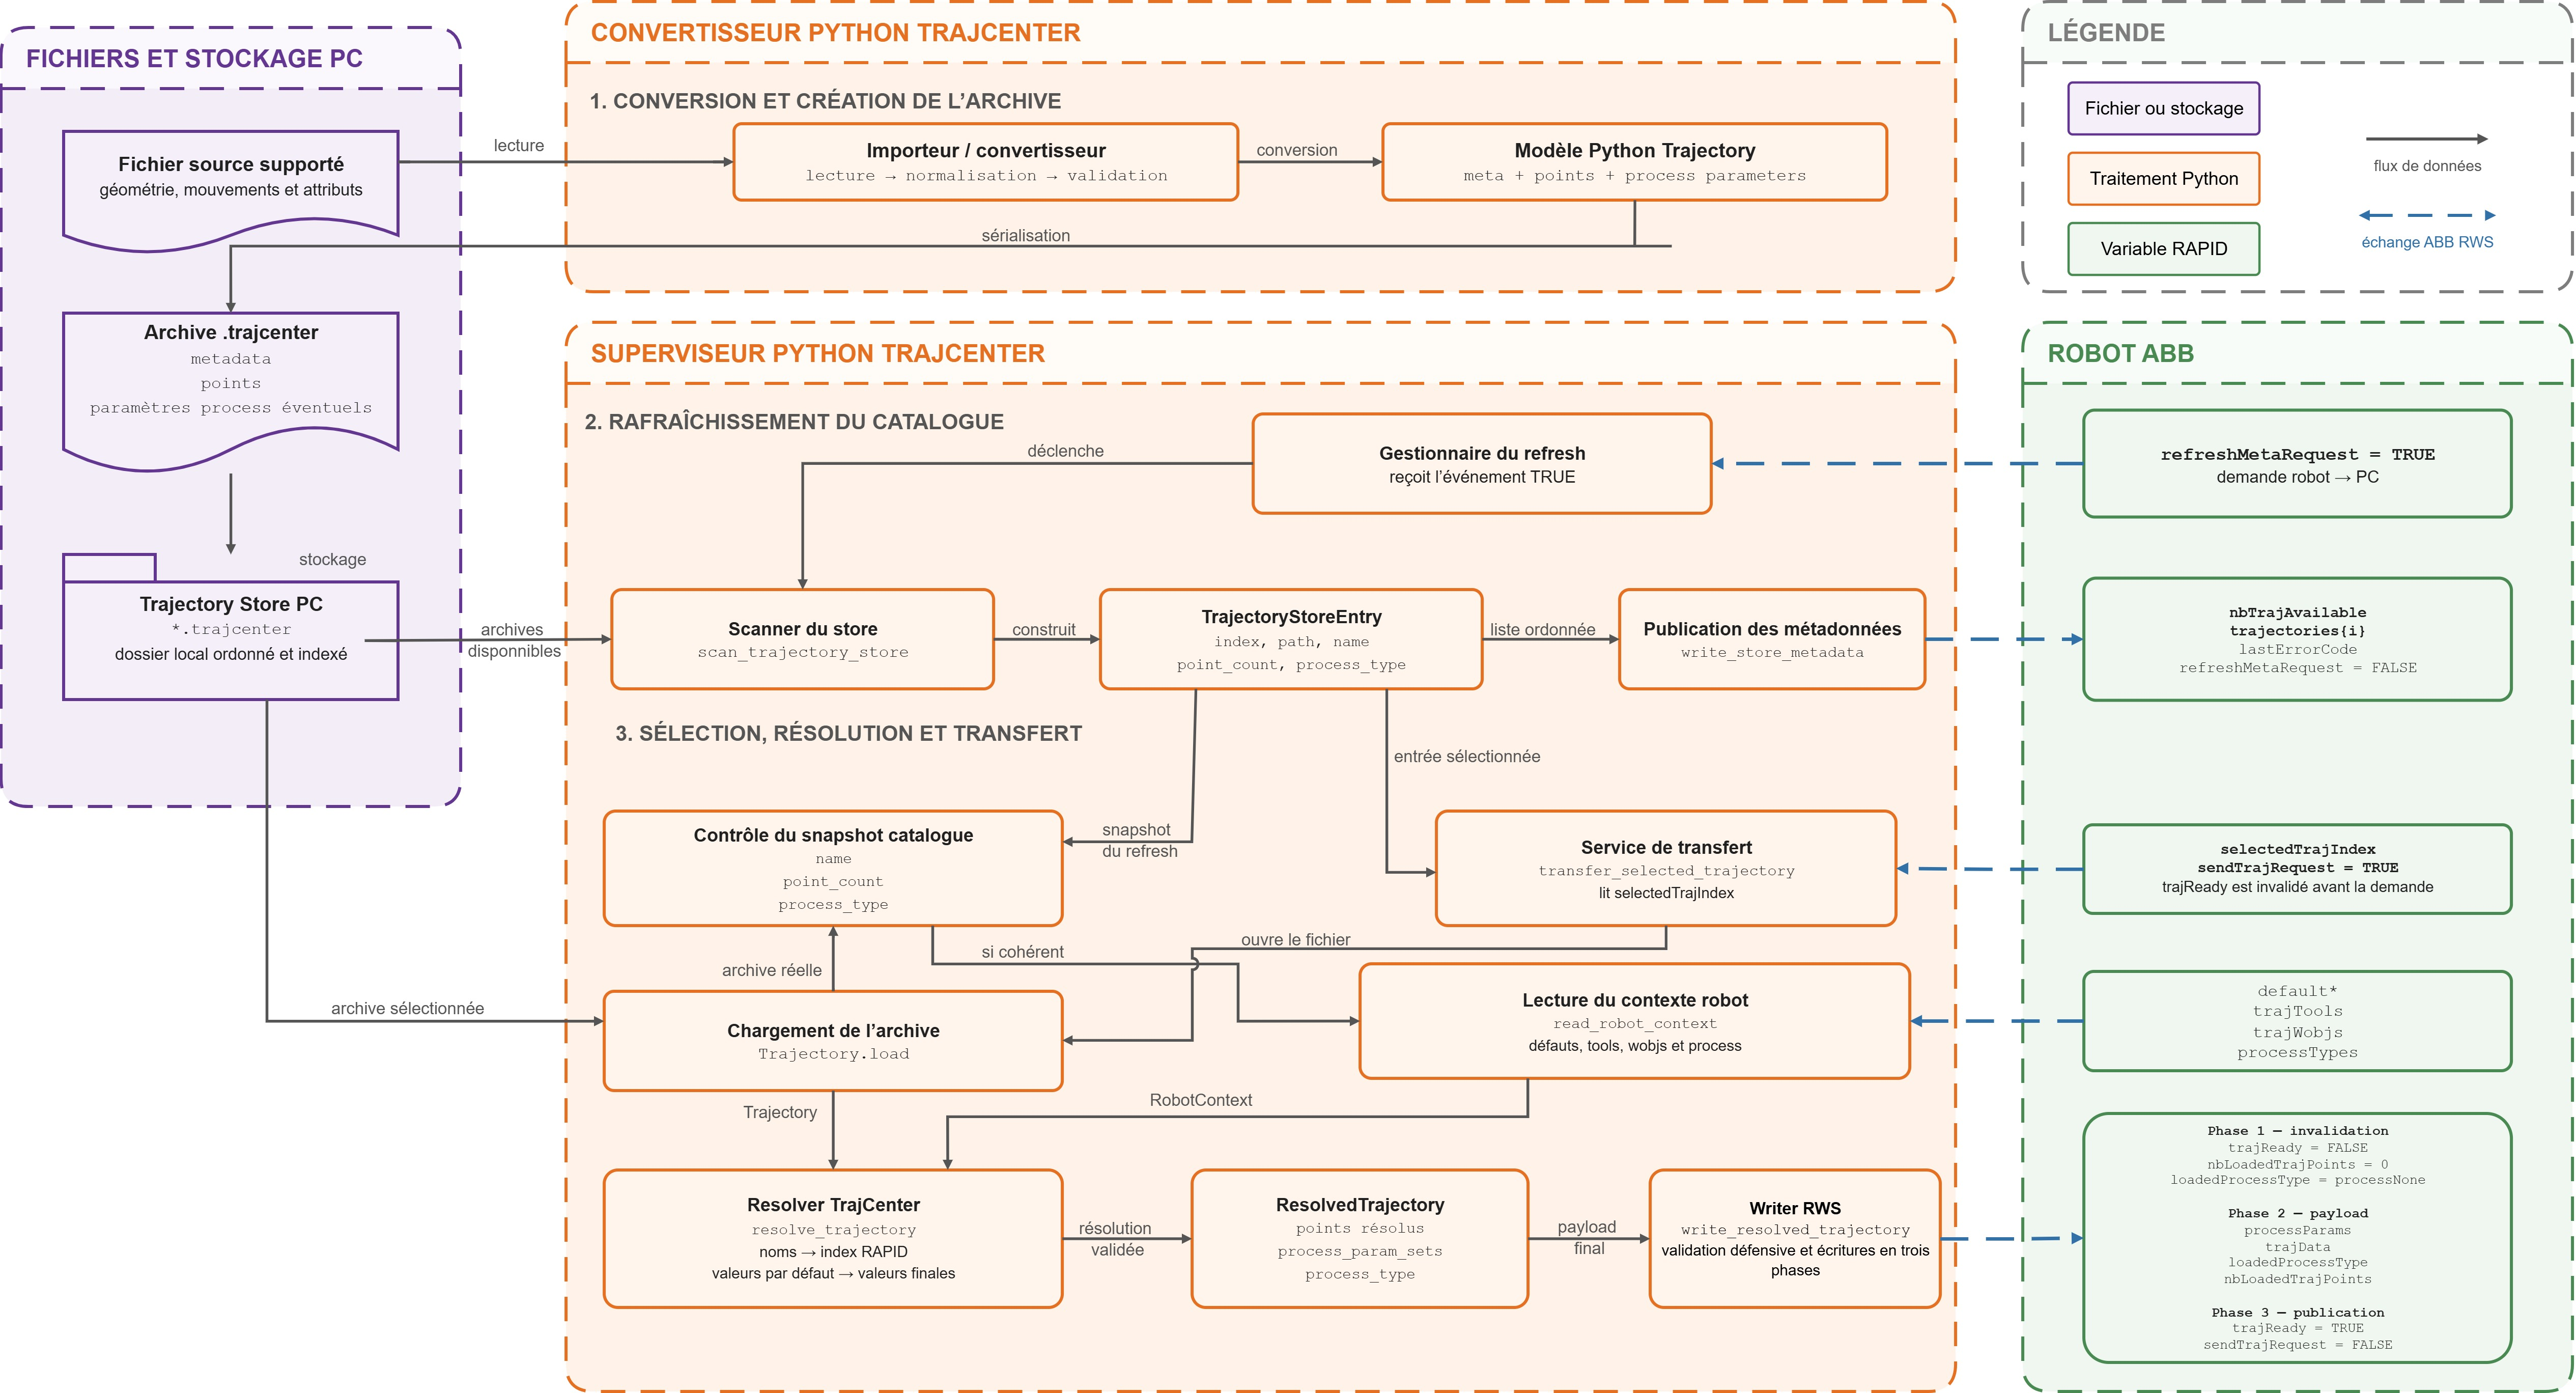
\includegraphics[
        width=\linewidth,
        keepaspectratio
    ]{figures/schema/trajcenter_architecture}
    \caption{Flux de données TrajCenter entre le store PC, Python et RAPID}
    \label{fig:rapid-module-architecture}
\end{sidewaysfigure}

Cette figure représente un \textbf{flux de données}. Elle ne doit pas être
interprétée comme un graphe d'appels de fonctions.

Le cycle général est le suivant :

\begin{enumerate}
    \item un fichier source est converti en archive
    \texttt{.trajcenter} ;
    \item l'archive est placée dans le store local ;
    \item le superviseur scanne le store et construit le catalogue ;
    \item le catalogue est publié dans
    \texttt{nbTrajAvailable} et \texttt{trajectories} ;
    \item le robot sélectionne une entrée du catalogue ;
    \item Python charge l'archive effectivement sélectionnée ;
    \item Python vérifie sa cohérence avec le snapshot du catalogue ;
    \item Python lit les defaults, les tools, les workobjects et le catalogue
    process du contrôleur ;
    \item le resolver produit une trajectoire entièrement résolue ;
    \item le writer valide le payload puis l'écrit dans RAPID.
\end{enumerate}

Les flèches bleues entre Python et RAPID représentent les échanges utilisant
ABB Robot Web Services. RWS est un canal de communication et non un composant
physique intermédiaire.

Le transfert d'une trajectoire suit un protocole en trois phases :

\begin{enumerate}
    \item \textbf{invalidation} :
    \texttt{trajReady} passe à \texttt{FALSE},
    \texttt{nbLoadedTrajPoints} passe à \texttt{0} et
    \texttt{loadedProcessType} revient à \texttt{processNone} ;
    \item \textbf{écriture du payload} :
    Python écrit \texttt{processParams}, \texttt{trajData},
    \texttt{loadedProcessType} et \texttt{nbLoadedTrajPoints} ;
    \item \textbf{publication} :
    Python met \texttt{trajReady} à \texttt{TRUE}, puis remet
    \texttt{sendTrajRequest} à \texttt{FALSE}.
\end{enumerate}

Ainsi, les anciennes valeurs éventuellement présentes dans les tableaux ne
sont jamais considérées comme valides tant que \texttt{trajReady} ne vaut pas
\texttt{TRUE}.

Le programme RAPID utilisateur ne doit pas écrire directement dans :

\begin{itemize}
    \item \texttt{trajectories} ;
    \item \texttt{trajData} ;
    \item \texttt{processParams} ;
    \item \texttt{loadedProcessType} ;
    \item \texttt{nbLoadedTrajPoints} ;
    \item les variables d'état gérées par le protocole.
\end{itemize}

Ces données sont alimentées par le superviseur sous Mastership ou modifiées par
les routines internes du module.


\subsubsection{Validité du payload chargé}
\label{subsubsec:rapid-loaded-payload-validity}

La validité du payload est représentée par trois variables principales :

\begin{itemize}
    \item \texttt{trajReady} indique si le payload complet est publiable ;
    \item \texttt{nbLoadedTrajPoints} indique la plage valide dans
    \texttt{trajData} ;
    \item \texttt{loadedProcessType} indique le process associé au payload
    effectivement chargé.
\end{itemize}

La routine interne \texttt{TRAJCENTER\_InvalidateLoaded} applique l'état
d'invalidation suivant :

\begin{lstlisting}[
    style=rapid,
    caption={État d'invalidation du payload chargé},
    label={lst:rapid-loaded-payload-invalidation}
]
trajReady := FALSE;
nbLoadedTrajPoints := 0;
loadedProcessType := processNone;
\end{lstlisting}

Les tableaux \texttt{trajData} et \texttt{processParams} ne sont pas
nécessairement effacés. Leurs anciennes valeurs deviennent simplement
inaccessibles, car leurs compteurs et leur indicateur de validité ne permettent
plus de les utiliser.

Le payload est invalidé notamment :

\begin{itemize}
    \item avant une nouvelle demande de trajectoire ;
    \item lorsqu'un tool est ajouté ou modifié ;
    \item lorsqu'un workobject est ajouté ou modifié ;
    \item lorsqu'un tool ou un workobject est supprimé ;
    \item lorsque la configuration cellule est vidée ;
    \item lorsqu'un transfert échoue avant sa publication complète.
\end{itemize}

La routine \texttt{TRAJCENTER\_RequestMetaRefresh} n'invalide pas le payload
chargé. Un rafraîchissement du catalogue peut donc être réalisé sans rendre
inexécutable une trajectoire déjà publiée, tant que la configuration de cellule
associée à cette trajectoire n'est pas modifiée.


\subsubsection{Compatibilité des versions}
\label{subsubsec:rapid-version-compatibility}

Les dimensions et structures du module RAPID doivent être compatibles avec le
profil de protocole pris en charge par la version Python installée.

Le fichier interne Python
\texttt{trajcenter/robot/constants.py} n'est pas un fichier de configuration
utilisateur. Il décrit les conventions et capacités attendues par cette version
du logiciel.

Une modification portant sur les éléments suivants nécessite une évolution
coordonnée :

\begin{itemize}
    \item dimensions des tableaux ;
    \item types RECORD ;
    \item ordre des champs dans les RECORD ;
    \item noms ou emplacement des variables RWS ;
    \item codes d'état et d'erreur ;
    \item représentation des types de mouvement ;
    \item identifiants des types de process ;
    \item structure des paramètres process.
\end{itemize}

Dans la version décrite par ce manuel, la capacité maximale d'une trajectoire
est fixée à \texttt{10000} points côté Python et côté RAPID. Les constantes
correspondantes doivent rester strictement alignées.

Toutes les dimensions du module RAPID ne sont pas nécessairement comparées
automatiquement avec le profil Python au démarrage. Le module
\texttt{TRAJCENTER.sys} et le logiciel Python doivent donc être déployés dans
des versions compatibles.


%==============================================================================
\subsection{API RAPID publique}
\label{subsec:rapid-public-api}
%==============================================================================

Le tableau~\ref{tab:rapid-main-routines} résume les principales routines
destinées aux programmes de cellule.

\begin{table}[ht]
    \centering
    \small
    \begin{tabularx}{\linewidth}{
        |p{0.34\linewidth}
        |p{0.23\linewidth}
        |X|
    }
        \hline
        \textbf{Routine} &
        \textbf{Arguments} &
        \textbf{Utilisation} \\
        \hline

        \texttt{TRAJCENTER\_InitErrors} &
        Aucun &
        Initialise les erreurs RAPID locales. \\
        \hline

        \texttt{TRAJCENTER\_InitCellConfig} &
        Aucun &
        Ajoute ou met à jour \texttt{tool0} et \texttt{wobj0}. \\
        \hline

        \texttt{TRAJCENTER\_UpsertTool} &
        \texttt{string}, \texttt{tooldata} &
        Ajoute ou met à jour un tool et invalide le payload chargé. \\
        \hline

        \texttt{TRAJCENTER\_UpsertWobj} &
        \texttt{string}, \texttt{wobjdata} &
        Ajoute ou met à jour un workobject et invalide le payload chargé. \\
        \hline

        \texttt{TRAJCENTER\_DeleteTool} &
        \texttt{string} &
        Supprime un tool et invalide le payload chargé. \\
        \hline

        \texttt{TRAJCENTER\_DeleteWobj} &
        \texttt{string} &
        Supprime un workobject et invalide le payload chargé. \\
        \hline

        \texttt{TRAJCENTER\_ClearTools} &
        Aucun &
        Vide les tools exposés et invalide le payload chargé. \\
        \hline

        \texttt{TRAJCENTER\_ClearWobjs} &
        Aucun &
        Vide les workobjects exposés et invalide le payload chargé. \\
        \hline

        \texttt{TRAJCENTER\_ClearCellConfig} &
        Aucun &
        Vide les tools et workobjects exposés. \\
        \hline

        \texttt{TRAJCENTER\_RequestMetaRefresh} &
        Aucun &
        Demande le rafraîchissement du catalogue sans invalider le payload
        chargé. \\
        \hline

        \texttt{TRAJCENTER\_WaitRequestDone} &
        \texttt{num timeoutSec} &
        Attend la fin d'une requête de rafraîchissement. \\
        \hline

        \texttt{TRAJCENTER\_RequestTrajectory} &
        \texttt{num trajIndex} &
        Invalide le payload courant et demande une trajectoire par index. \\
        \hline

        \texttt{TRAJCENTER\_RequestTrajByName} &
        \texttt{string trajName} &
        Recherche une trajectoire par nom puis la demande par index. \\
        \hline

        \texttt{TRAJCENTER\_WaitTrajectoryReady} &
        \texttt{num timeoutSec} &
        Attend la publication complète du payload. \\
        \hline

        \texttt{TRAJCENTER\_GetLoadedPointCount} &
        Aucun &
        Retourne le nombre de points valides. \\
        \hline

        \texttt{TRAJCENTER\_GetPoint} &
        \texttt{num},
        \texttt{VAR trajCenterPointData} &
        Copie un point chargé dans une variable utilisateur. \\
        \hline

        \texttt{TRAJCENTER\_GetTool} &
        \texttt{num},
        \texttt{VAR tooldata} &
        Copie un tool dans une variable utilisateur. \\
        \hline

        \texttt{TRAJCENTER\_GetWobj} &
        \texttt{num},
        \texttt{VAR wobjdata} &
        Copie un workobject dans une variable utilisateur. \\
        \hline

        \texttt{TRAJCENTER\_PointHasProcessParams} &
        \texttt{num pointIndex} &
        Indique si un point référence un jeu de paramètres process. \\
        \hline

        \texttt{TRAJCENTER\_GetProcessParam} &
        Point, nom et variables de sortie &
        Recherche un paramètre process numérique associé à un point. \\
        \hline

        \texttt{TRAJCENTER\_ExecuteLoaded} &
        Trois valeurs \texttt{num} &
        Exécute le payload chargé avec le process indiqué par
        \texttt{loadedProcessType}. \\
        \hline
    \end{tabularx}
    \caption{Principales routines publiques de TrajCenter}
    \label{tab:rapid-main-routines}
\end{table}

La routine \texttt{TRAJCENTER\_ExecuteLoaded} est l'unique point d'entrée
recommandé pour l'exécution. Il n'existe plus d'API d'exécution séparée pour
les trajectoires sans process.

Une trajectoire sans process correspond au cas suivant :

\begin{lstlisting}[
    style=rapid,
    caption={Représentation d'une trajectoire sans process},
    label={lst:rapid-none-process}
]
loadedProcessType = processNone
\end{lstlisting}

Les signatures exactes doivent toujours être vérifiées dans le module
\texttt{TRAJCENTER.sys} correspondant à la version installée.


%==============================================================================
\subsection{Intégration des paramètres process}
\label{subsec:rapid-process-integration}
%==============================================================================

Les paramètres process sont transférés dans le tableau
\texttt{processParams}. Chaque point peut référencer un jeu de paramètres au
moyen de son champ \texttt{processParamIndex}.

La convention est la suivante :

\begin{itemize}
    \item \texttt{processParamIndex = 0} signifie qu'aucun jeu de paramètres
    n'est associé au point ;
    \item une valeur comprise entre \texttt{1} et
    \texttt{maxProcessParamSetCount} référence une ligne de
    \texttt{processParams} ;
    \item dans un jeu, un nom vide indique un slot inutilisé ;
    \item les paramètres process transportés par le protocole sont numériques.
\end{itemize}


\subsubsection{Catalogue des process exécutables}
\label{subsubsec:rapid-process-limitations}

Le tableau \texttt{processTypes} représente les process réellement
exécutables par le contrôleur. Le superviseur Python lit ce catalogue avant
d'accepter une trajectoire.

Dans la version actuelle du module :

\begin{lstlisting}[
    style=rapid,
    caption={Catalogue process actuellement publié},
    label={lst:rapid-current-process-catalog}
]
CONST num processTypeCount := 1;

VAR trajCenterProcessType processTypes{processTypeCount}:=[
    [processNone, "NONE"]
];
\end{lstlisting}

Les identifiants \texttt{processAcf}, \texttt{processAak} et
\texttt{processPushcorp} sont réservés dans le module, mais ils ne sont pas
publiés dans le catalogue. Leurs routines \texttt{Begin} lèvent encore
\texttt{ERR\_TRAJCENTER\_PROCESS\_NOT\_IMPLEMENTED}.

Une trajectoire utilisant l'un de ces process doit donc être refusée par le
superviseur tant que son implémentation RAPID n'est pas opérationnelle et que
le process n'a pas été ajouté à \texttt{processTypes}.


\subsubsection{Accès contrôlé aux paramètres process}
\label{subsubsec:technic-process-parameter-access}

Les routines process doivent utiliser \texttt{TRAJCENTER\_PointHasProcessParams} et \texttt{TRAJCENTER\_GetProcessParam} plutôt que lire directement les tableaux internes.

L'exemple suivant recherche un paramètre numérique associé au point courant :

\begin{lstlisting}[
    style=rapid,
    caption={Lecture d'un paramètre process pour un point},
    label={lst:rapid-get-process-param}
]
VAR bool found;
VAR num processValue;

TRAJCENTER_GetProcessParam
    pointIndex,
    "example_parameter",
    found,
    processValue;

IF found = FALSE THEN
    RAISE ERR_TRAJCENTER_BAD_PROCESS_PARAM_INDEX;
ENDIF
\end{lstlisting}

Cette API centralise :

\begin{itemize}
    \item le contrôle de l'index du point ;
    \item le contrôle de l'index du jeu de paramètres ;
    \item la recherche du paramètre par son nom ;
    \item la distinction entre paramètre absent et valeur numérique nulle.
\end{itemize}


\subsubsection{Implémentation d'un process métier}
\label{subsubsec:rapid-custom-process-execution}

L'ajout d'un process ne nécessite pas de créer une nouvelle routine globale
d'exécution. Le moteur de mouvement est déjà fourni par
\texttt{TRAJCENTER\_ExecuteOneMotion}.

Chaque process doit implémenter cinq hooks :

\begin{description}
    \item[\texttt{Begin}] initialise le process avant le premier mouvement ;
    \item[\texttt{BeforeMotion}] applique les paramètres avant l'instruction
    de mouvement ;
    \item[\texttt{AfterMotion}] réalise les actions nécessaires après
    l'instruction de mouvement ;
    \item[\texttt{End}] termine normalement le process ;
    \item[\texttt{Abort}] remet le process dans un état sûr lorsqu'une erreur
    survient.
\end{description}

Pour ajouter un process, appliquer la séquence suivante :

\begin{enumerate}
    \item définir ou confirmer son identifiant dans la section~5 du module ;
    \item implémenter ses cinq routines process dans la section~9.10 ;
    \item ajouter les appels correspondants dans chacun des dispatchers de la
    section~9.11 ;
    \item ajouter le process dans le tableau \texttt{processTypes} ;
    \item incrémenter \texttt{processTypeCount} ;
    \item mettre à jour les constantes et validations Python ;
    \item ajouter les tests correspondants ;
    \item mettre à jour la documentation.
\end{enumerate}

Un process ne doit être ajouté à \texttt{processTypes} qu'une fois son
implémentation RAPID réellement utilisable.

Pour les hooks \texttt{BeforeMotion} et \texttt{AfterMotion}, l'index fourni
correspond au premier point du mouvement courant. Pour un \texttt{MoveC}, il
désigne le point de passage ; le point d'arrivée est situé à l'index suivant.

Les hooks sont appelés une fois par instruction de mouvement, et non une fois
par entrée du tableau \texttt{trajData}. Un \texttt{MoveC} consomme donc deux
entrées, mais provoque un seul appel à chaque hook.

Une action réalisée dans \texttt{AfterMotion} n'est pas nécessairement
synchronisée avec le passage physique exact au point lorsque la zone n'est pas
\texttt{fine}. Un procédé nécessitant une synchronisation précise doit
utiliser une stratégie ABB adaptée, par exemple des triggers, des instructions
process spécialisées ou un moteur dédié explicitement conçu pour cette
synchronisation.


%==============================================================================
\subsection{Routines internes et graphe d'appels}
\label{subsec:rapid-internal-routines}
%==============================================================================

Certaines routines RAPID sont présentes dans le module pour factoriser les
opérations internes. Elles ne font pas toutes partie du parcours d'utilisation
courant.

Le fait qu'une routine soit techniquement accessible depuis un programme RAPID
ne signifie pas qu'elle constitue une API publique stable. Les programmes de
cellule doivent privilégier les points d'entrée documentés.


\subsubsection{Principales routines de support}
\label{subsubsec:rapid-support-routines}

Les routines de support prennent notamment en charge :

\begin{itemize}
    \item l'invalidation du payload chargé ;
    \item la recherche des tools et workobjects ;
    \item la recherche d'une trajectoire par son nom ;
    \item la construction des données de vitesse ;
    \item la conversion des zones ;
    \item le chargement des caches d'exécution tool et workobject ;
    \item l'application de la politique \texttt{readConfs} ;
    \item l'accès contrôlé aux paramètres process ;
    \item la validation et l'exécution d'un mouvement ;
    \item le dispatch des appels process.
\end{itemize}

Les principales routines concernées sont :

\begin{itemize}
    \item \texttt{TRAJCENTER\_InvalidateLoaded} ;
    \item \texttt{TRAJCENTER\_FindToolIndex} ;
    \item \texttt{TRAJCENTER\_FindWobjIndex} ;
    \item \texttt{TRAJCENTER\_FindTrajectoryIndex} ;
    \item \texttt{TRAJCENTER\_MakeSpeed} ;
    \item \texttt{TRAJCENTER\_MakeZone} ;
    \item \texttt{TRAJCENTER\_LoadExecTool} ;
    \item \texttt{TRAJCENTER\_LoadExecWobj} ;
    \item \texttt{TRAJCENTER\_ApplyReadConfs} ;
    \item \texttt{TRAJCENTER\_ProcessBegin} ;
    \item \texttt{TRAJCENTER\_ProcessBeforeMotion} ;
    \item \texttt{TRAJCENTER\_ProcessAfterMotion} ;
    \item \texttt{TRAJCENTER\_ProcessEnd} ;
    \item \texttt{TRAJCENTER\_ProcessAbort} ;
    \item \texttt{TRAJCENTER\_ExecuteOneMotion}.
\end{itemize}


\subsubsection{Moteur commun de mouvement}
\label{subsubsec:rapid-common-motion-engine}

La routine \texttt{TRAJCENTER\_ExecuteOneMotion} constitue l'unique
implémentation générique des mouvements.

Pour chaque mouvement, elle :

\begin{enumerate}
    \item lit le point courant dans \texttt{trajData} ;
    \item construit le \texttt{speeddata} ;
    \item convertit la zone numérique en \texttt{zonedata} ;
    \item charge le tool dans \texttt{trajExecTool} ;
    \item charge le workobject dans \texttt{trajExecWobj} ;
    \item applique la politique \texttt{readConfs} ;
    \item appelle le hook \texttt{ProcessBeforeMotion} ;
    \item exécute \texttt{MoveL}, \texttt{MoveJ} ou \texttt{MoveC} ;
    \item appelle le hook \texttt{ProcessAfterMotion} ;
    \item avance l'index d'un ou de deux points.
\end{enumerate}

Pour un mouvement circulaire, la routine vérifie que les deux entrées
consécutives :

\begin{itemize}
    \item sont toutes les deux de type \texttt{moveTypeC} ;
    \item utilisent la même vitesse TCP ;
    \item utilisent le même tool ;
    \item utilisent le même workobject ;
    \item utilisent la même zone ;
    \item utilisent la même politique \texttt{readConfs} ;
    \item référencent le même jeu de paramètres process.
\end{itemize}


\subsubsection{Graphe d'appels}
\label{subsubsec:rapid-call-graph}

\begin{sidewaysfigure}
    \centering
    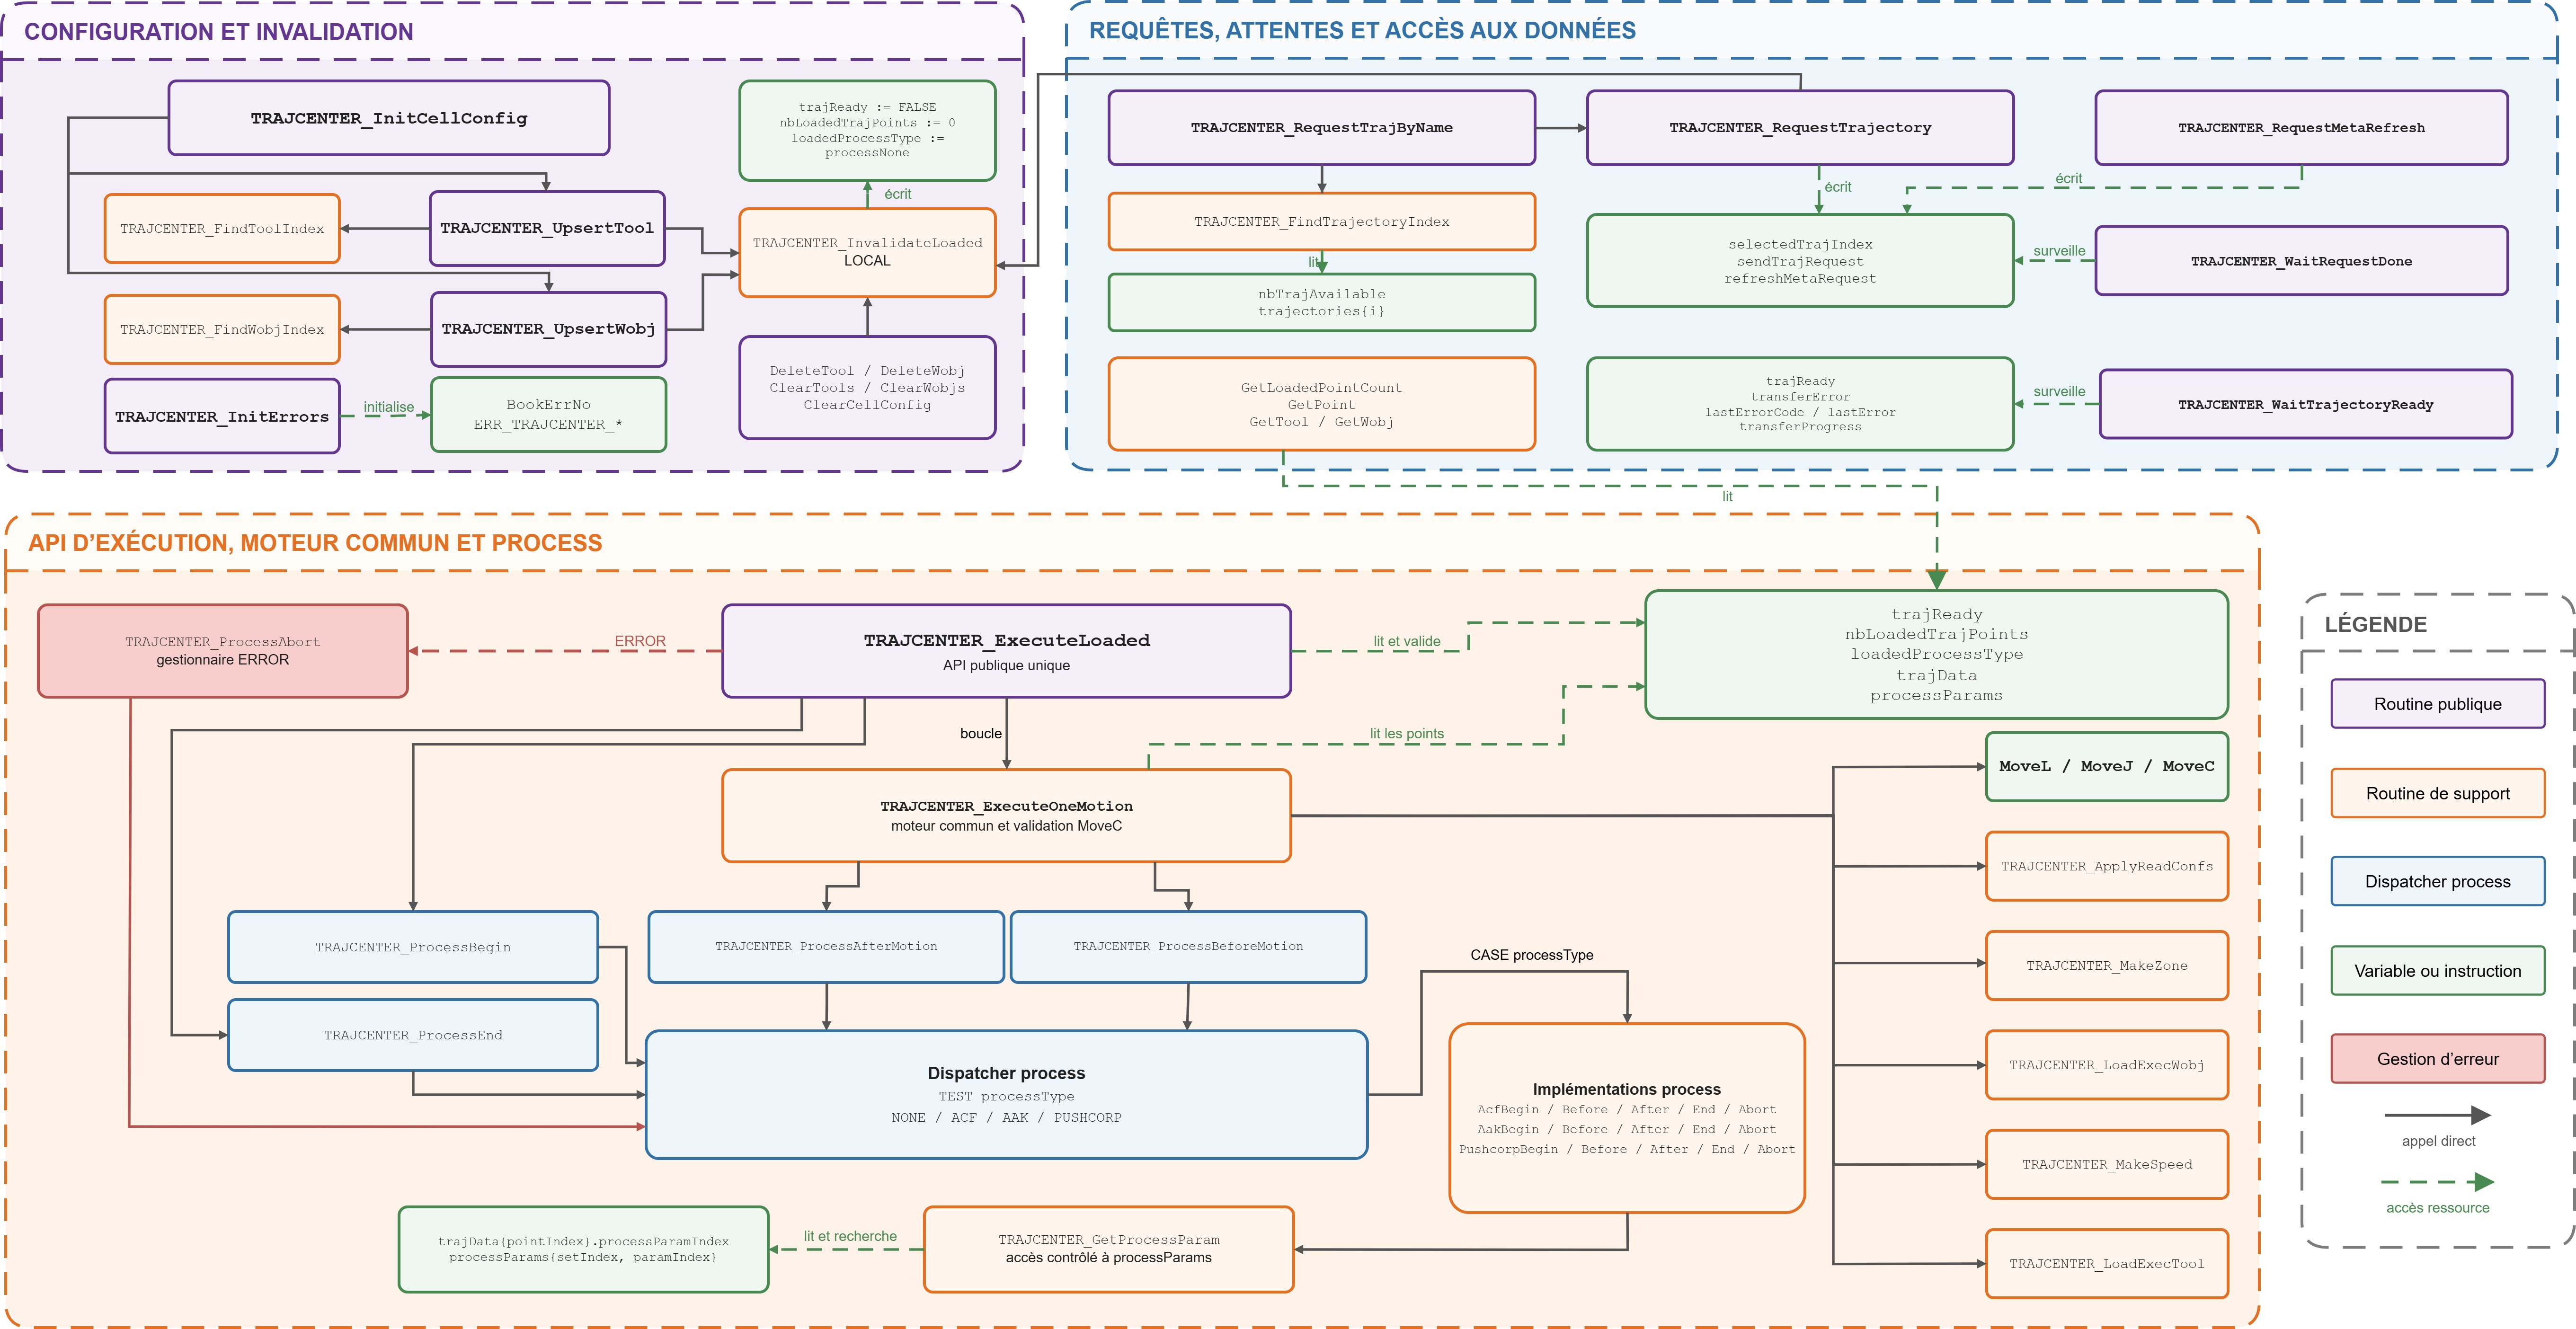
\includegraphics[
        width=\linewidth,
        keepaspectratio
    ]{figures/schema/rapid_api_call_graph}
    \caption{Graphe d'appels et interdépendances du module système RAPID}
    \label{fig:rapid-api-call-graph}
\end{sidewaysfigure}

La figure~\ref{fig:rapid-api-call-graph} présente une vue simplifiée des
appels et interdépendances internes du module système RAPID. Dans ce graphe :

\begin{itemize}
    \item une flèche pleine représente un appel direct entre routines RAPID ;
    \item une flèche verte en pointillés représente l'accès à une variable ou
    à une instruction RAPID ;
    \item une flèche rouge représente le chemin de gestion d'erreur ;
    \item une liaison d'extension indique une dépendance prévue pour une
    implémentation process.
\end{itemize}

La routine \texttt{TRAJCENTER\_ExecuteLoaded} organise l'exécution globale :

\begin{enumerate}
    \item elle vérifie \texttt{trajReady} et
    \texttt{nbLoadedTrajPoints} ;
    \item elle copie \texttt{loadedProcessType} dans une variable locale ;
    \item elle appelle \texttt{TRAJCENTER\_ProcessBegin} ;
    \item elle appelle \texttt{TRAJCENTER\_ExecuteOneMotion} jusqu'à la fin du
    payload ;
    \item elle appelle \texttt{TRAJCENTER\_ProcessEnd} ;
    \item elle restaure \texttt{ConfL} et \texttt{ConfJ} à
    \texttt{\textbackslash On}.
\end{enumerate}

Si une erreur survient, son gestionnaire \texttt{ERROR} :

\begin{enumerate}
    \item appelle \texttt{TRAJCENTER\_ProcessAbort} ;
    \item restaure \texttt{ConfL} et \texttt{ConfJ} ;
    \item propage l'erreur originale avec \texttt{RAISE}.
\end{enumerate}

Cette structure garantit que le process \texttt{NONE} et les futurs process
métier empruntent le même moteur de mouvement et la même stratégie de remise en
état.


%==============================================================================
\subsection{Règles de modification du module}
\label{subsec:rapid-module-modification-rules}
%==============================================================================

Une modification locale de la configuration de la cellule n'a pas le même
impact qu'une modification du protocole ou du moteur d'exécution.


\subsubsection{Modifications propres à la cellule}
\label{subsubsec:rapid-cell-local-changes}

Les opérations suivantes relèvent normalement de l'intégration de la cellule :

\begin{itemize}
    \item ajouter ou mettre à jour un tool ;
    \item ajouter ou mettre à jour un workobject ;
    \item choisir les valeurs par défaut ;
    \item configurer les équipements associés à un process ;
    \item compléter les hooks d'un process déjà réservé ;
    \item associer des sorties, instructions ou données métier aux hooks
    process.
\end{itemize}

Ces opérations ne doivent pas modifier la structure des variables échangées
avec Python.

Toute modification d'un tool ou d'un workobject invalide le payload chargé.
La trajectoire doit alors être redemandée avant toute nouvelle exécution.


\subsubsection{Ajout ou activation d'un process}
\label{subsubsec:rapid-process-changes}

L'activation d'un process doit être réalisée de manière coordonnée :

\begin{enumerate}
    \item confirmer son identifiant numérique ;
    \item implémenter ses cinq hooks RAPID ;
    \item compléter les cinq dispatchers ;
    \item vérifier que son hook \texttt{Abort} ne masque pas l'erreur
    originale ;
    \item ajouter le process à \texttt{processTypes} ;
    \item incrémenter \texttt{processTypeCount} ;
    \item mettre à jour les constantes et validations Python ;
    \item ajouter des trajectoires et tests représentatifs ;
    \item mettre à jour la documentation.
\end{enumerate}

La simple présence d'une constante telle que \texttt{processAcf} ne signifie
pas que le process est disponible. Seules les entrées valides de
\texttt{processTypes} constituent le catalogue publié au superviseur.


\subsubsection{Modifications du protocole}
\label{subsubsec:rapid-protocol-changes}

Les opérations suivantes constituent une évolution du protocole :

\begin{itemize}
    \item changer les dimensions des tableaux ;
    \item modifier un type RECORD échangé ;
    \item modifier l'ordre des champs d'un RECORD ;
    \item ajouter, supprimer ou renommer une variable RWS ;
    \item modifier la représentation d'un type de mouvement ;
    \item modifier les identifiants des process ;
    \item modifier les codes d'état ou d'erreur ;
    \item modifier la structure des paramètres process ;
    \item modifier le protocole d'invalidation et de publication du payload.
\end{itemize}

Elles doivent être réalisées simultanément :

\begin{enumerate}
    \item dans le module RAPID ;
    \item dans le client Python ;
    \item dans les constantes et validations Python ;
    \item dans les tests unitaires et d'intégration ;
    \item dans les démonstrations RAPID ;
    \item dans la documentation utilisateur et technique ;
    \item dans la gestion de version du module et du logiciel.
\end{enumerate}

Il ne faut pas utiliser le fichier \texttt{.env} pour contourner une
incompatibilité de dimensions ou de structures. Le fichier
\texttt{.env} configure la connexion et le superviseur ; il ne redéfinit pas
le protocole.

\FloatBarrier


\end{document}
